\documentclass[10pt,aspectratio=169]{beamer}
% ====================================================================
% Deck doble: DEFENSA (examen de titulo) y CONFERENCIA (paper IEEE).
%   - Defensa (por defecto):   pdflatex defensa.tex
%   - Conferencia:             pdflatex -jobname=charla_conferencia "\def\confmode{1}\documentclass[10pt,aspectratio=169]{beamer}
% ====================================================================
% Deck doble: DEFENSA (examen de titulo) y CONFERENCIA (paper IEEE).
%   - Defensa (por defecto):   pdflatex defensa.tex
%   - Conferencia:             pdflatex -jobname=charla_conferencia "\def\confmode{1}\documentclass[10pt,aspectratio=169]{beamer}
% ====================================================================
% Deck doble: DEFENSA (examen de titulo) y CONFERENCIA (paper IEEE).
%   - Defensa (por defecto):   pdflatex defensa.tex
%   - Conferencia:             pdflatex -jobname=charla_conferencia "\def\confmode{1}\documentclass[10pt,aspectratio=169]{beamer}
% ====================================================================
% Deck doble: DEFENSA (examen de titulo) y CONFERENCIA (paper IEEE).
%   - Defensa (por defecto):   pdflatex defensa.tex
%   - Conferencia:             pdflatex -jobname=charla_conferencia "\def\confmode{1}\input{defensa.tex}"
% Solo cambian portada/autores/afiliacion/evento; el contenido es el mismo.
% ====================================================================
\providecommand{\confmode}{0}% 0 = defensa, 1 = conferencia
\usepackage[utf8]{inputenc}
\usepackage[T1]{fontenc}
\usepackage[spanish,es-noquoting]{babel}
% Evita el "Incompatible glue units" de babel-spanish al usar \% dentro de beamer
\makeatletter
\let\es@sppercent\relax
\makeatother
\usepackage{graphicx}
\usepackage{booktabs}
\usepackage{amsmath}
\usepackage{xcolor}

\graphicspath{{figuras/}}

% --- Metadatos (usados por la plantilla oficial en portada, pie y cabecera) ---
\ifnum\confmode=1
  % ----- Modo CONFERENCIA (paper IEEE) -----
  \title[Pronóstico FV \emph{Cold-Start} · LOPO]{Pronóstico fotovoltaico a corto plazo bajo escasez de datos mediante evaluación \emph{Leave-One-Plant-Out}}
  \subtitle{Un enfoque \emph{Cross-Site} multi-planta frente a modelos locales}
  \author[Aular \& Hernández]{César David Aular Muñoz \and Sergio Hernández}
  \institute[UCM]{Departamento de Computación e Industrias \\ Facultad de Ciencias de la Ingeniería \\ Universidad Católica del Maule}
  \date{Chilean Workshop on Pattern Recognition (CWPR) --- 2026}
\else
  % ----- Modo DEFENSA (examen de título) -----
  \title[Multi-sitio vs.\ local: pronóstico FV \emph{Cold-Start}]{Análisis comparativo de un enfoque multi-sitio frente a modelos locales para la proyección a corto plazo de generación fotovoltaica bajo escasez de datos}
  % \subtitle{Proyección a corto plazo de generación fotovoltaica bajo escasez de datos}
  \author[César Aular]{César David Aular Muñoz}
  \institute[Escuela ICI --- UCM]{Escuela Ingeniería Civil Informática \\ Universidad Católica del Maule}
  \date{Proyecto de Título --- Junio 2026}
\fi

% --- Plantilla oficial de presentación UCM (tema QUT: azul institucional #00407a) ---
\usepackage{QUT}

% --- Colores semánticos: global (azul) / local (verde) / alerta (rojo) ---
\definecolor{glob}{HTML}{1F77B4}
\definecolor{loc}{HTML}{2CA02C}
\definecolor{alertred}{HTML}{C0392B}
\newcommand{\gl}[1]{\textcolor{glob}{\textbf{#1}}}
\newcommand{\lo}[1]{\textcolor{loc}{\textbf{#1}}}
\newcommand{\rj}[1]{\textcolor{alertred}{\textbf{#1}}}

% --- Bloques redondeados con relleno (info=azul UCM / ejemplo=verde / alerta=rojo) ---
\setbeamertemplate{blocks}[rounded][shadow=true]
\setbeamercolor{block title}{bg=qut,fg=white}
\setbeamercolor{block body}{bg=qut!8,fg=black}
\setbeamercolor{block title example}{bg=loc,fg=white}
\setbeamercolor{block body example}{bg=loc!8,fg=black}
\setbeamercolor{block title alerted}{bg=alertred,fg=white}
\setbeamercolor{block body alerted}{bg=alertred!8,fg=black}

\begin{document}

\begin{frame}[plain]
  \titlepage
  \begin{center}
    
\includegraphics[width=0.16\linewidth]{figuras/logoUCM.png}
  \end{center}
\end{frame}

\begin{frame}{Agenda}
  \tableofcontents[hideallsubsections]
\end{frame}

% ==================================================================
\section{El problema}
% ==================================================================

\begin{frame}{El problema del \emph{Cold-Start} fotovoltaico}
  \begin{columns}[T]
    \begin{column}{0.56\textwidth}
      \begin{itemize}
        \item Una planta FV \textbf{recién conectada} no tiene historial de generación.
        \item Los modelos clásicos entrenan \textbf{uno por planta} con meses o años de datos locales.
        \item Aplicados a una planta nueva: \rj{no se pueden entrenar} o se degradan gravemente.
      \end{itemize}
      \vspace{0.4em}
      \begin{alertblock}{Consecuencia}
        Incertidumbre justo cuando más se necesita certeza $\rightarrow$ mayores costos de balance y riesgo financiero, en especial para los pequeños PMGD.
      \end{alertblock}
    \end{column}
    \begin{column}{0.44\textwidth}
      \centering
      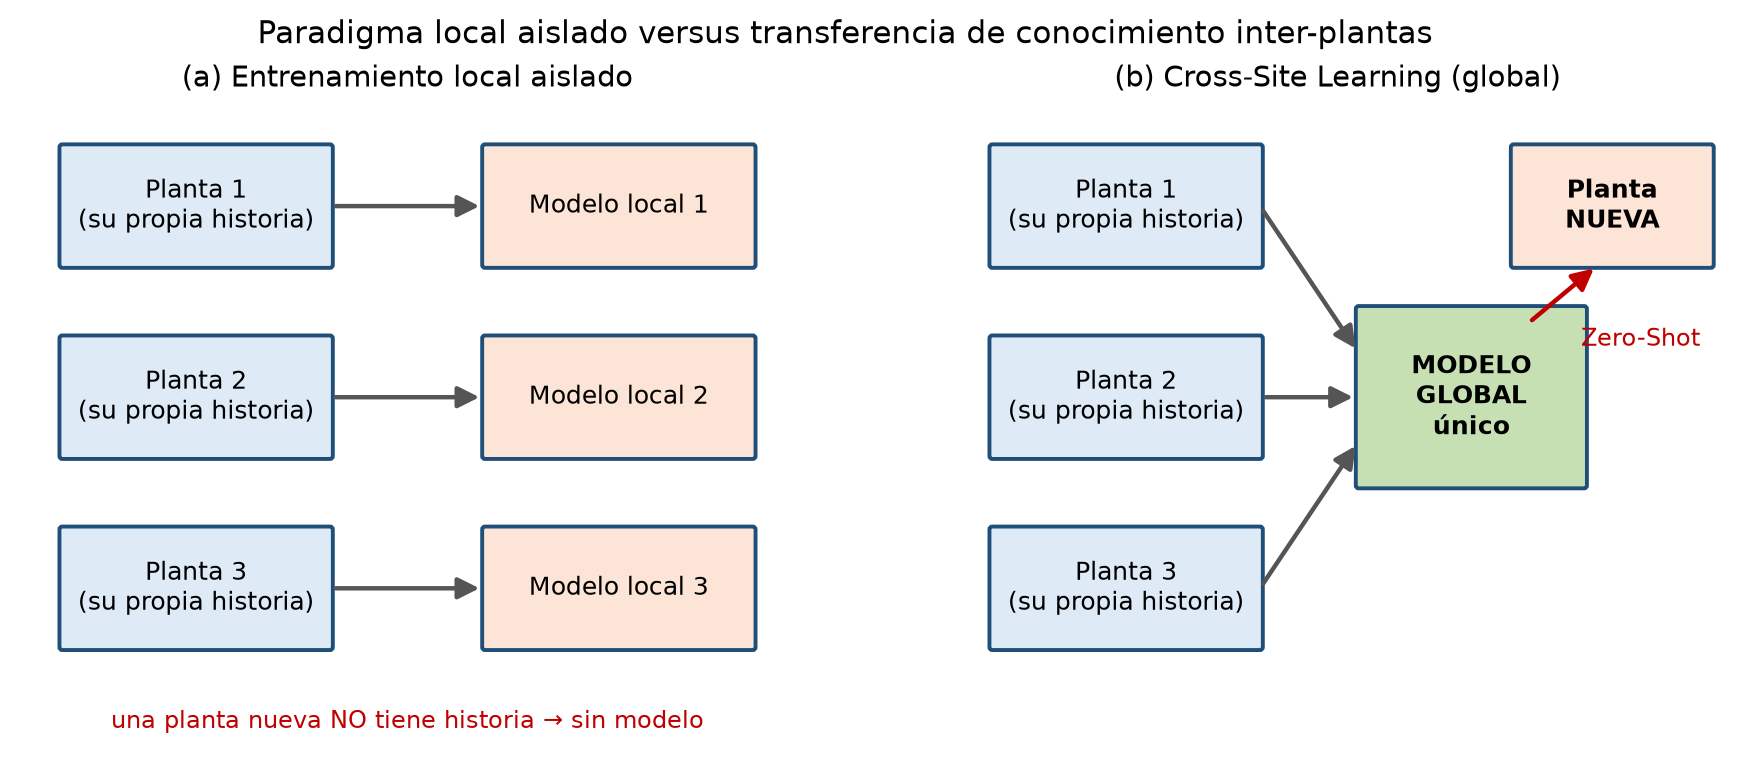
\includegraphics[width=\linewidth]{fig_cross_site.png}
      \vspace{0.3em}

      {\footnotesize El problema del arranque en frío, tomado de los sistemas de recomendación.}
    \end{column}
  \end{columns}
\end{frame}

\begin{frame}{La idea: aprendizaje \emph{Cross-Site}}
  \begin{columns}[T]
    \begin{column}{0.5\textwidth}
      Abandonar el supuesto \textbf{un-modelo-por-planta}.

      \vspace{0.6em}
      Un único modelo \gl{global} entrenado sobre \textbf{muchas plantas a la vez}:
      \begin{itemize}
        \item absorbe patrones compartidos clima~$\rightarrow$~potencia,
        \item los \textbf{transfiere} a una planta jamás vista,
        \item pronostica \textbf{desde la primera hora} de conexión.
      \end{itemize}
      \vspace{0.5em}
      \textbf{Pregunta central (adversarial):}\\
      \emph{¿realmente supera a una línea base local madura, o el premio de la transferencia se desvanece con una comparación justa?}
    \end{column}
    \begin{column}{0.5\textwidth}
      \centering
      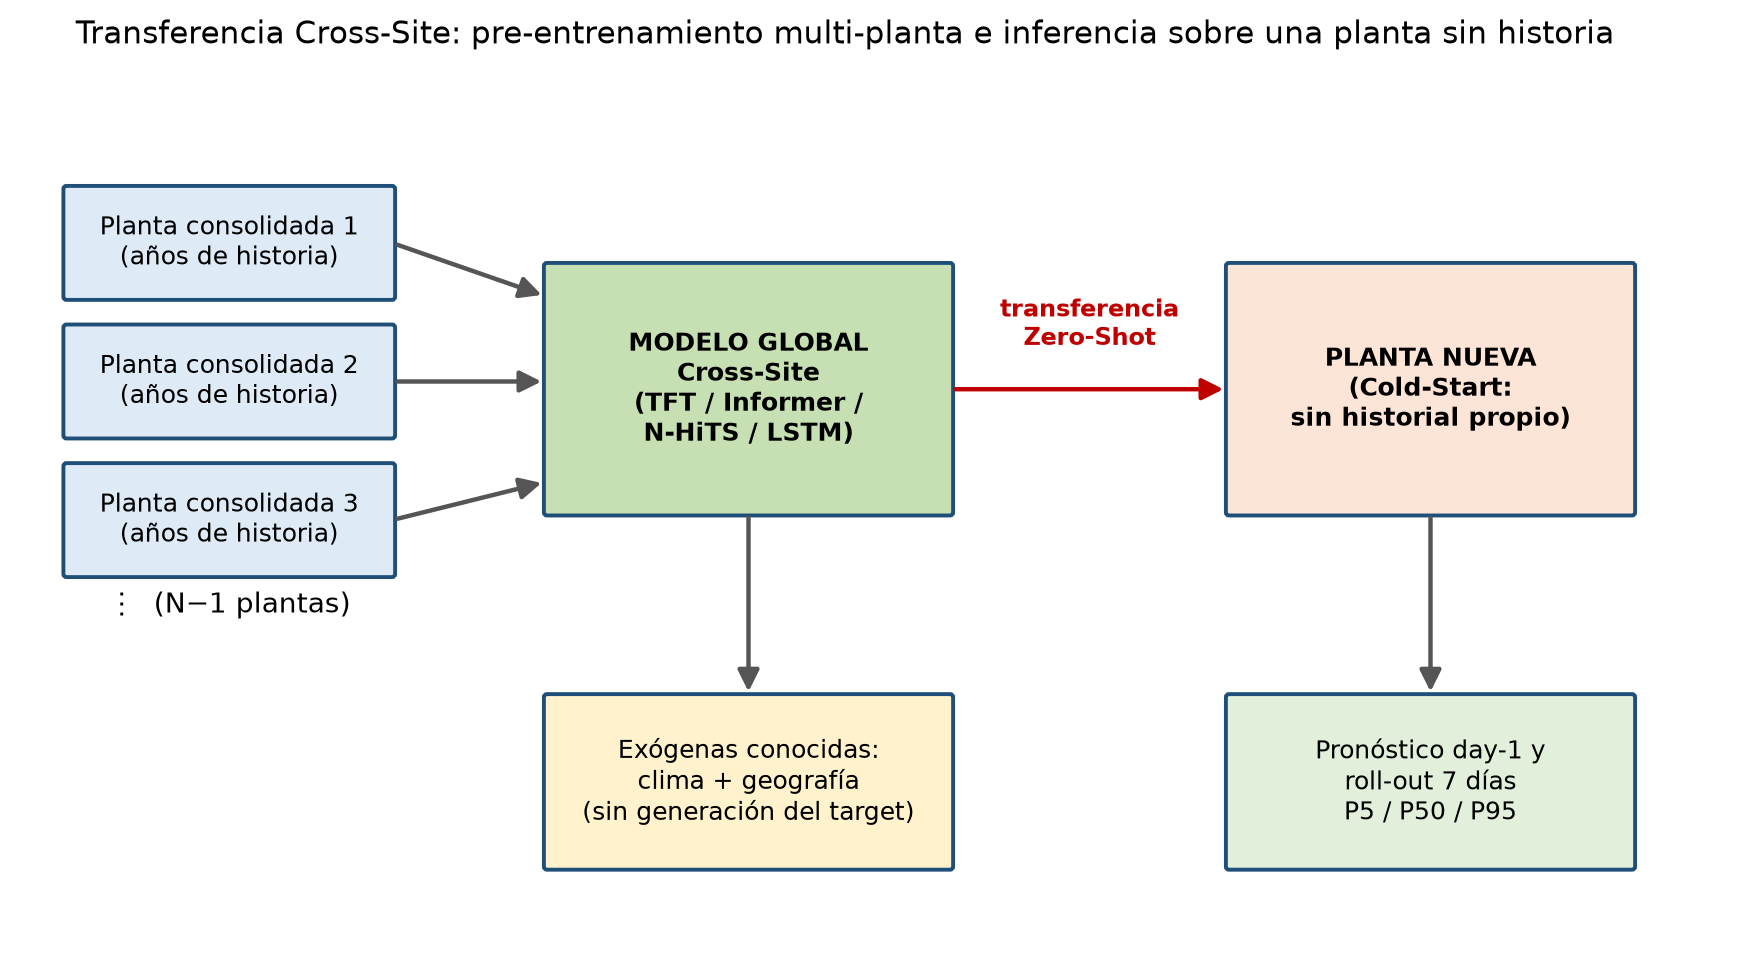
\includegraphics[width=\linewidth]{fig_solucion.png}
    \end{column}
  \end{columns}
\end{frame}

\begin{frame}{Hipótesis y objetivos}
  \begin{block}{Hipótesis}
    El modelo global multi-sitio es \emph{más preciso} que un modelo entrenado localmente con la historia propia del centro.
  \end{block}
  \begin{columns}[T]
    \begin{column}{0.5\textwidth}
      \textbf{Objetivos específicos}
      \begin{enumerate}
        \item Adaptar una arquitectura Transformer al entrenamiento multi-serie.
        \item Evaluarla frente a modelos locales bajo un protocolo \emph{Cold-Start} estricto.
        \item Integrar datos multimodales sin fuga de información.
      \end{enumerate}
    \end{column}
    \begin{column}{0.5\textwidth}
      \textbf{La brecha en la literatura}\\
      Rara vez se combinan a la vez:
      \begin{enumerate}
        \item evaluación \textbf{ciega} a la planta objetivo (sin \emph{fine-tuning}),
        \item contraste \textbf{justo} contra locales maduros,
        \item caracterización \textbf{probabilística}.
      \end{enumerate}
    \end{column}
  \end{columns}
\end{frame}

% ==================================================================
\section{Metodología}
% ==================================================================

\begin{frame}{Arquitectura del sistema}
  \centering
  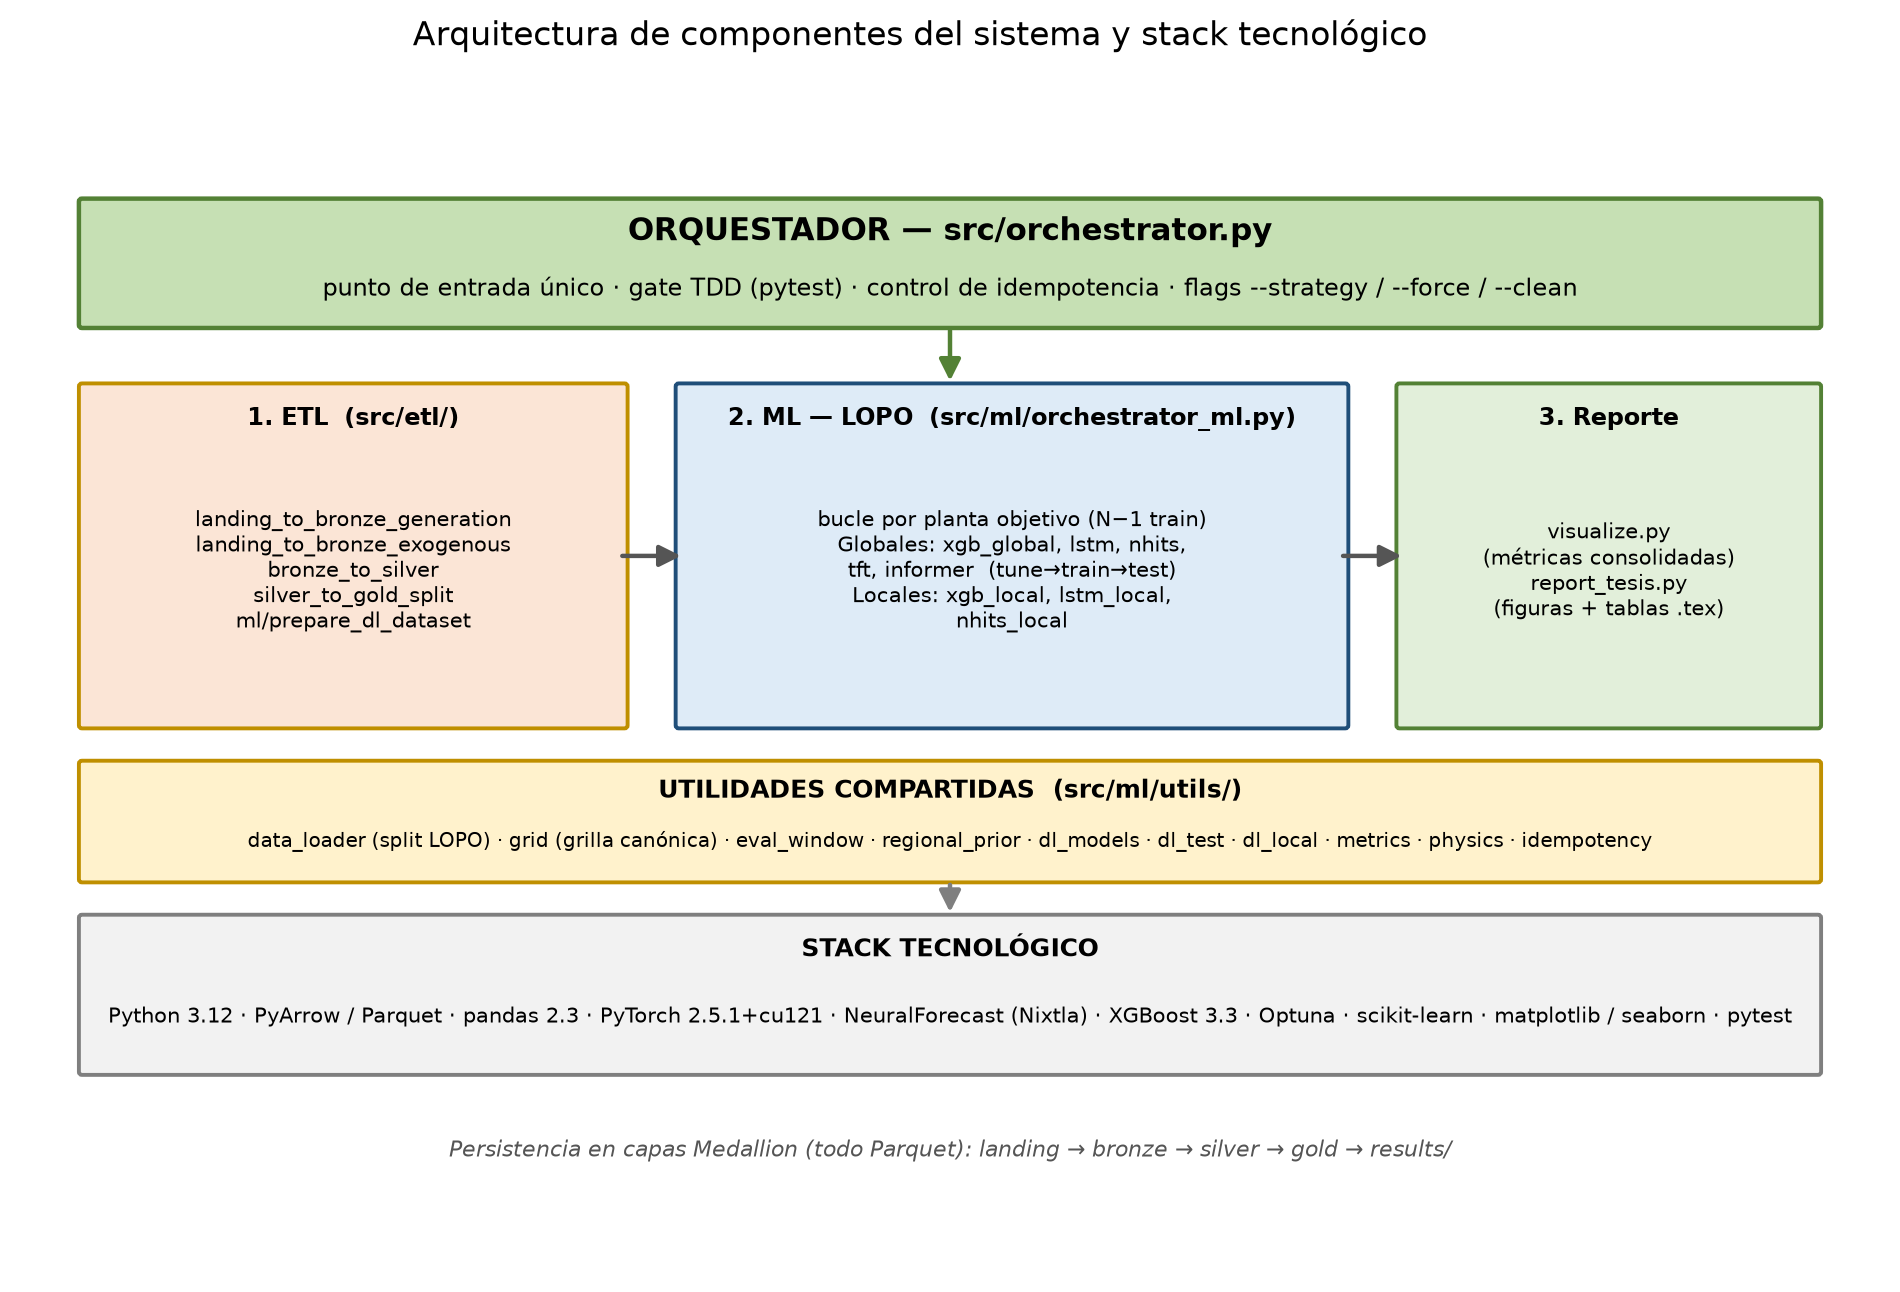
\includegraphics[height=0.78\textheight,keepaspectratio]{fig_arquitectura_componentes.png}
\end{frame}

\begin{frame}{Protocolo \emph{Leave-One-Plant-Out} (LOPO)}
  \begin{columns}[T]
    \begin{column}{0.52\textwidth}
      \begin{itemize}
        \item Para cada planta objetivo: los globales entrenan con las \textbf{$N-1$ restantes} (2014--2024 completo).
        \item La planta objetivo es \rj{invisible} durante el entrenamiento.
        \item Métricas: \textbf{mediana} sobre 94 plantas, solo observaciones reales.
      \end{itemize}
      \begin{exampleblock}{Integridad Zero-Shot (no negociable)}
        Ninguna variable puede ser función de la generación del objetivo. Verificado por pruebas automatizadas.
      \end{exampleblock}
    \end{column}
    \begin{column}{0.48\textwidth}
      \centering
      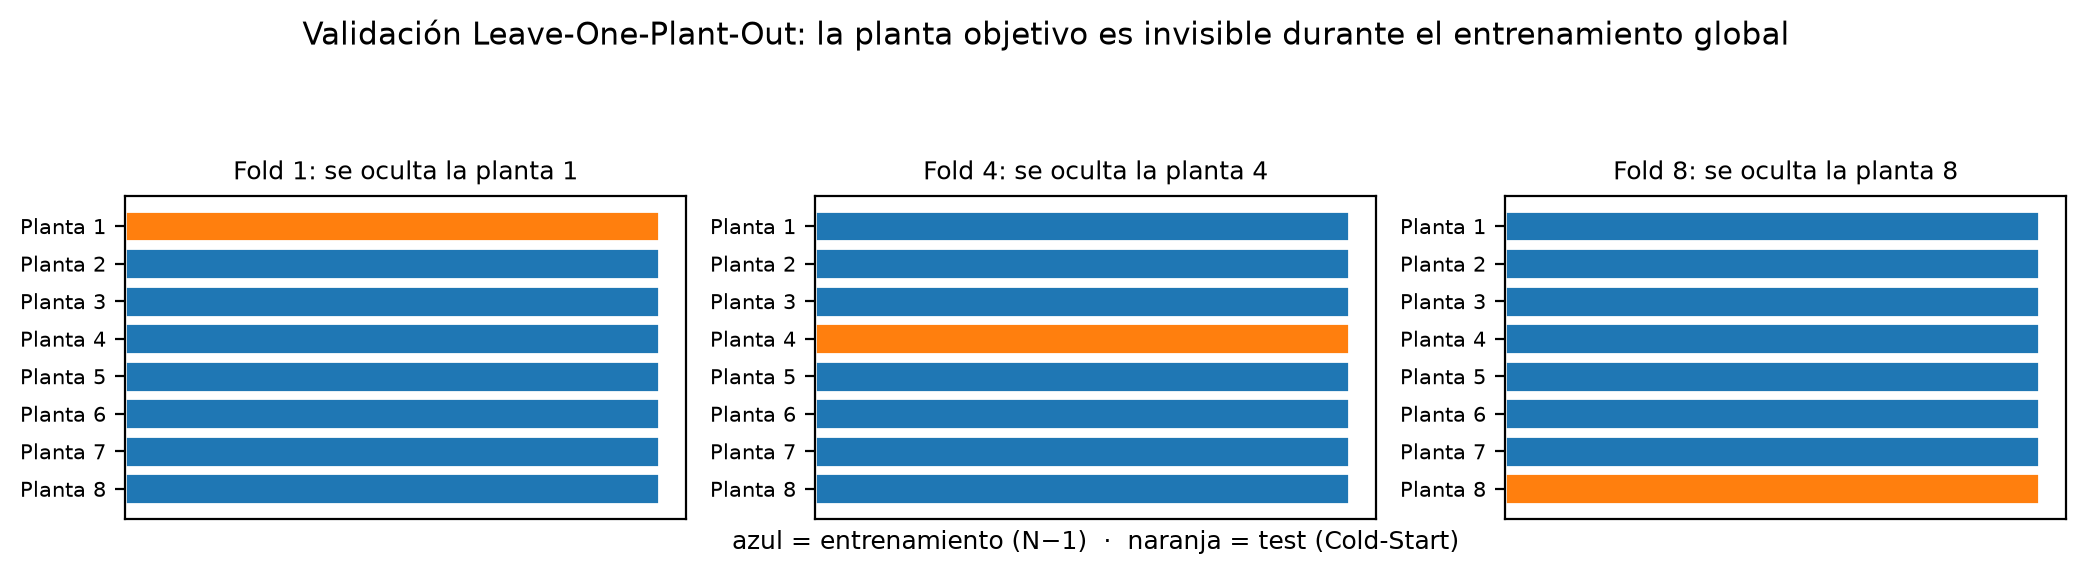
\includegraphics[width=\linewidth]{fig_lopo.png}
    \end{column}
  \end{columns}
\end{frame}

\begin{frame}{La lección de la fuga de datos}
  \begin{center}
    \Large Un \emph{prior} de eficiencia calculado \textbf{por-fila} desde el objetivo
  \end{center}
  \vspace{0.3em}
  \[
    PR = \frac{y}{\text{capacidad}} \quad\Longrightarrow\quad \mathrm{corr}(PR,\,y)=1.0
  \]
  \vspace{0.2em}
  \begin{columns}[T]
    \begin{column}{0.5\textwidth}
      \begin{alertblock}{rRMSE falso}
        $\approx 0.8\,\%$ \; (demasiado bueno para ser verdad)
      \end{alertblock}
    \end{column}
    \begin{column}{0.5\textwidth}
      \begin{exampleblock}{rRMSE honesto (tras corregir)}
        $\approx 56\,\%$
      \end{exampleblock}
    \end{column}
  \end{columns}
  \vspace{0.6em}
  \centering
  El \emph{prior} regional se agrega \textbf{solo sobre las plantas de entrenamiento} (por macrozona y estación).
\end{frame}

\begin{frame}{Semilla \emph{Cold-Start} sintética}
  Los modelos profundos necesitan una ventana de contexto que la planta nueva no tiene. Se siembra sintéticamente:
  \[
    \hat{y}_{\text{seed}}(t) = \text{capacidad}\cdot PR_{\text{regional}}\cdot s(t)
  \]
  \begin{itemize}
    \item $s(t)$: perfil solar determinista; $PR_{\text{regional}}$: solo plantas de entrenamiento.
    \item Solo el clima exógeno (conocido/pronosticable) y la geografía estática usan valores reales del objetivo.
    \item La generación de contexto es \rj{100\% sintética} $\rightarrow$ cero fuga.
  \end{itemize}
  \vspace{-0.4em}
  \centering
  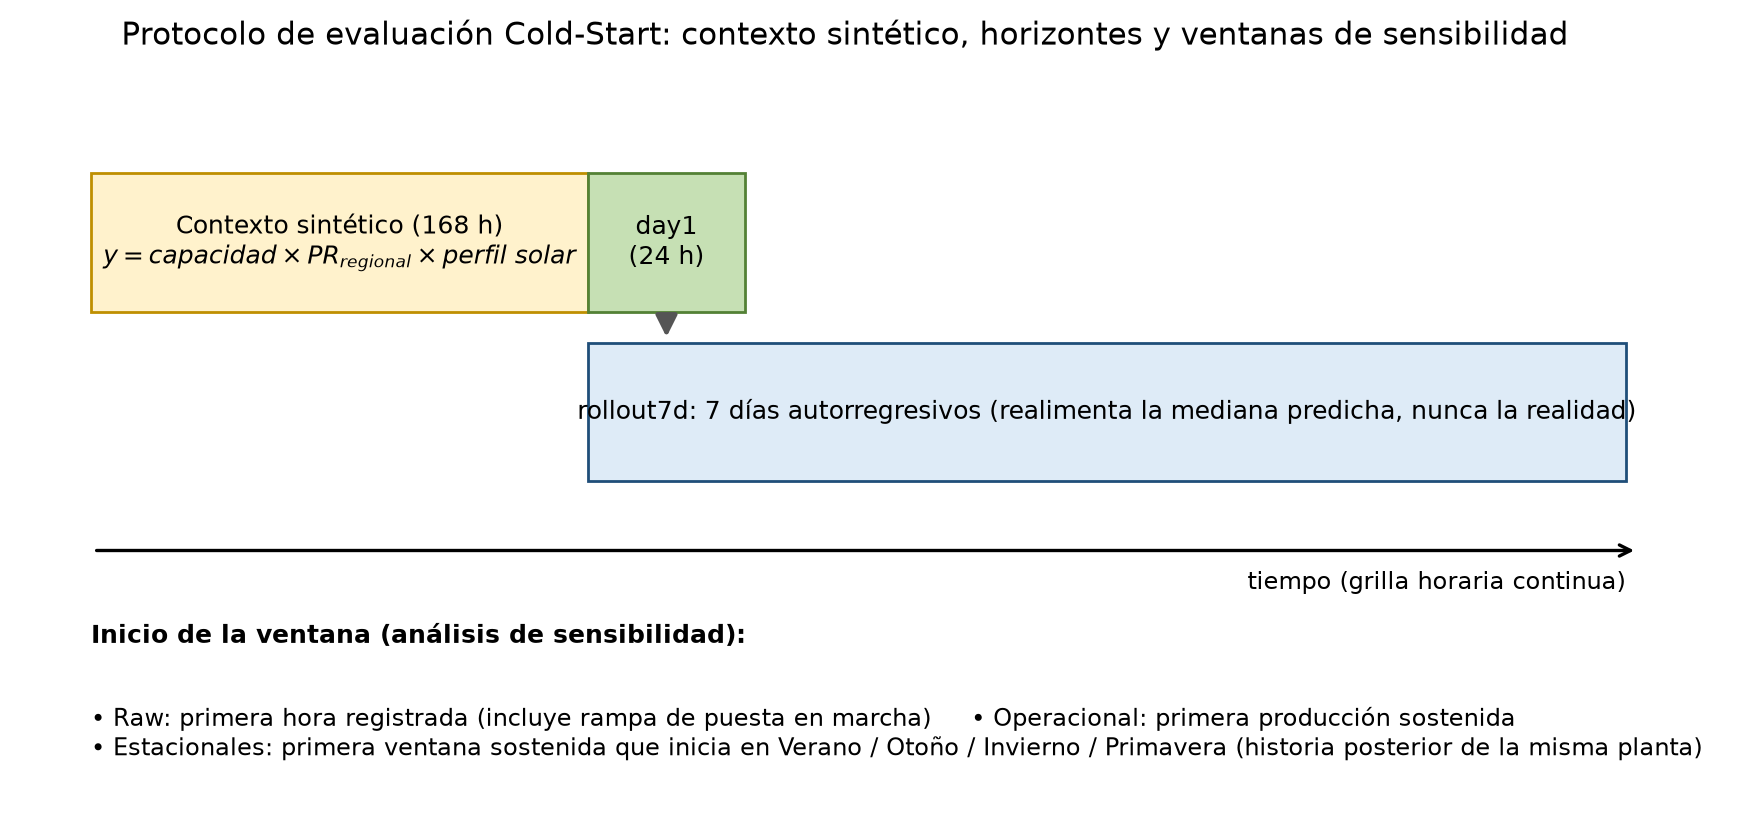
\includegraphics[width=0.54\textwidth]{fig_eval_protocolo.png}
\end{frame}

\begin{frame}{Ocho configuraciones y ventanas de evaluación}
  \begin{columns}[T]
    \begin{column}{0.48\textwidth}
      \textbf{5 globales \gl{(Cross-Site)}}
      \begin{itemize}
        \item TFT, Informer, N-HiTS, LSTM
        \item XGBoost global
      \end{itemize}
      \vspace{0.4em}
      \textbf{3 locales \lo{(estrictas)}}
      \begin{itemize}
        \item XGBoost, LSTM, N-HiTS
        \item entrenados solo con la historia propia
      \end{itemize}
      \vspace{0.5em}
      \textbf{Horizontes:} \emph{day1} (24\,h) y \emph{rollout7d} (7 días autorregresivos).
    \end{column}
    \begin{column}{0.52\textwidth}
      \centering
      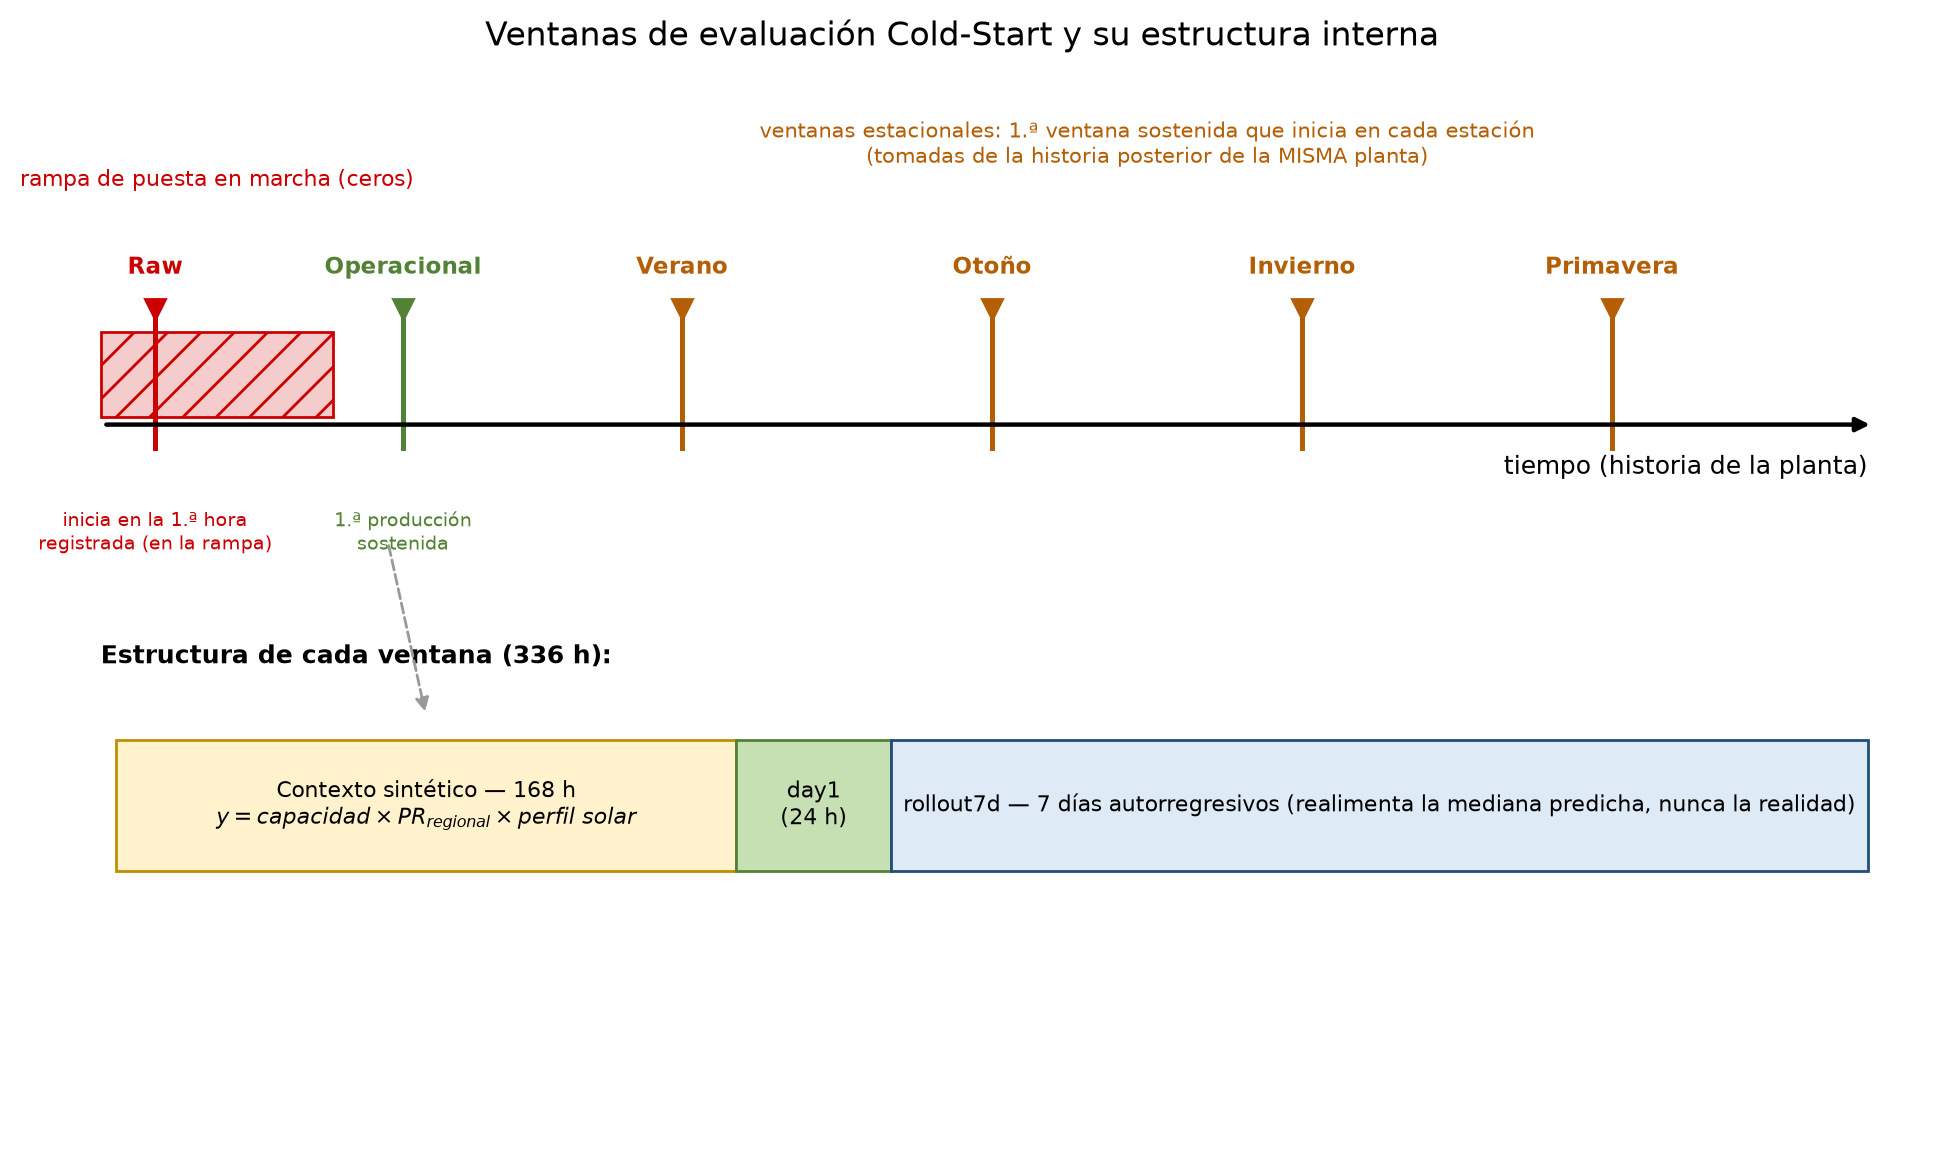
\includegraphics[width=\linewidth]{fig_ventanas_evaluacion.png}
      \vspace{0.2em}

      {\footnotesize \textbf{Raw} (incluye rampa) · \textbf{Operacional} (producción sostenida) · \textbf{Estacionales}.}
    \end{column}
  \end{columns}
\end{frame}

\begin{frame}{¿Dónde están las plantas? El corpus sobre el mapa}
  \begin{columns}[T]
    \begin{column}{0.42\textwidth}
      \centering
      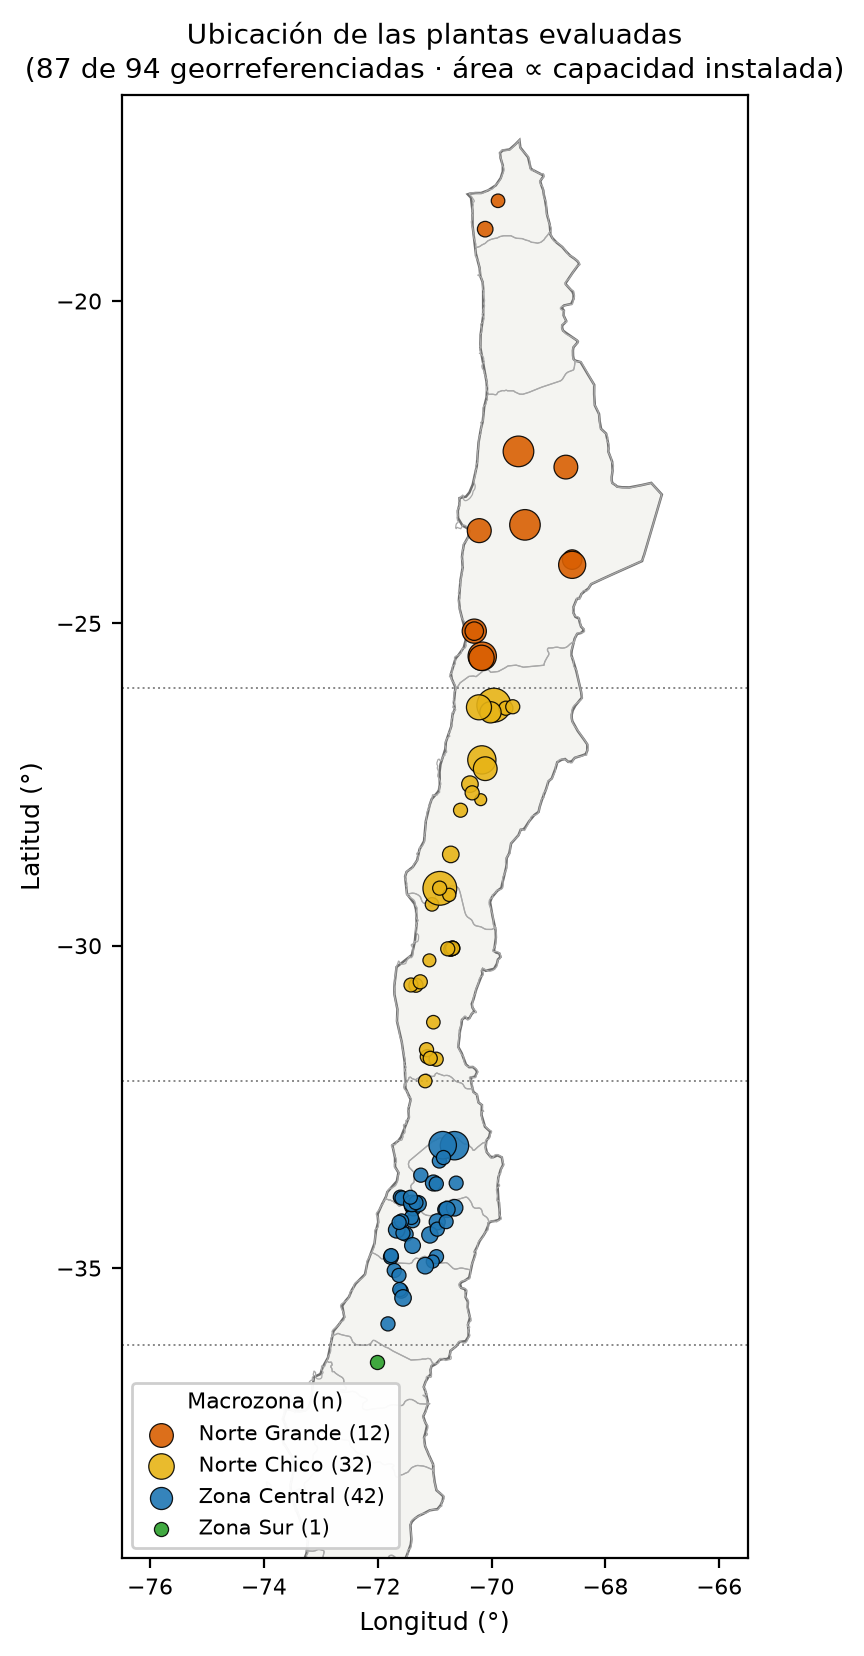
\includegraphics[height=0.78\textheight]{fig_mapa_plantas.png}
    \end{column}
    \begin{column}{0.58\textwidth}
      \vspace{1.2em}
      \begin{itemize}
        \item \textbf{94 plantas} del Sistema Eléctrico Nacional, a lo largo de todo el
              gradiente solar de Chile (Arica $\rightarrow$ zona sur).
        \item \gl{Norte Grande y Norte Chico}: pocas plantas pero \textbf{grandes}
              (utility scale, hasta 200\,MW) y de alta irradiancia.
        \item \lo{Zona Central}: muchas plantas \textbf{pequeñas} (PMGD, mediana
              $\approx$3\,MW) — el segmento que más sufre el arranque en frío.
      \end{itemize}
      \vspace{0.4em}
      \begin{exampleblock}{Por qué importa para la transferencia}
        La \textbf{macrozona} es la única señal espacial que ven los modelos, y es la
        clave sobre la que se agrega el \emph{prior} regional que siembra el contexto
        sintético.
      \end{exampleblock}
    \end{column}
  \end{columns}
\end{frame}

% ==================================================================
\section{Resultados}
% ==================================================================

\begin{frame}{Precisión puntual --- ventana \emph{cold-start}, 94 plantas (roll-out 7 días)}
  \begin{columns}[T]
    \begin{column}{0.46\textwidth}
      \small
      \begin{tabular}{llrr}
        \toprule
        Config. & Tipo & NRMSE & rRMSE \\
        \midrule
        XGBoost & \lo{Local}  & \textbf{13,2\,\%} & 60\,\% \\
        XGBoost & \gl{Global} & 17,1\,\% & 75\,\% \\
        N-HiTS  & \lo{Local}  & 17,6\,\% & 85\,\% \\
        Informer& \gl{Global} & 22,8\,\% & 107\,\% \\
        TFT     & \gl{Global} & 23,6\,\% & 113\,\% \\
        LSTM    & \lo{Local}  & 23,9\,\% & 129\,\% \\
        LSTM    & \gl{Global} & 24,8\,\% & 109\,\% \\
        N-HiTS  & \gl{Global} & 30,7\,\% & 148\,\% \\
        \bottomrule
      \end{tabular}

      \vspace{0.3em}
      {\scriptsize NRMSE = RMSE / capacidad instalada. \textbf{94 plantas}.}
    \end{column}
    \begin{column}{0.54\textwidth}
      \centering
      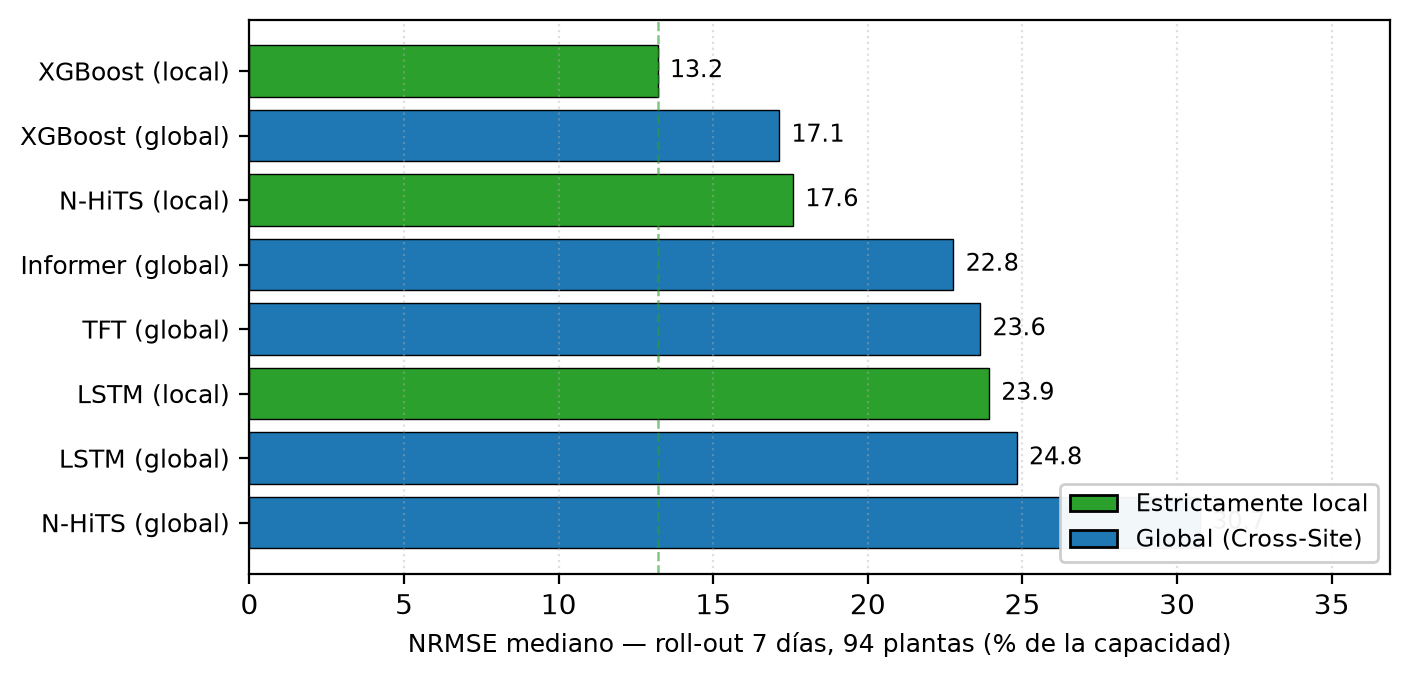
\includegraphics[width=\linewidth]{fig_resultados_nrmse_es.png}
    \end{column}
  \end{columns}
  \vspace{0.2em}
  {\footnotesize El \lo{XGBoost local} es el más preciso (13\,\% de la potencia nominal). Normalizar por \textbf{capacidad} hace los números interpretables —y cambia el orden del par LSTM respecto de rRMSE.}
\end{frame}

\begin{frame}{Sensibilidad estacional: el invierno es el gran desafío}
  \begin{columns}[T]
    \begin{column}{0.5\textwidth}
      \centering
      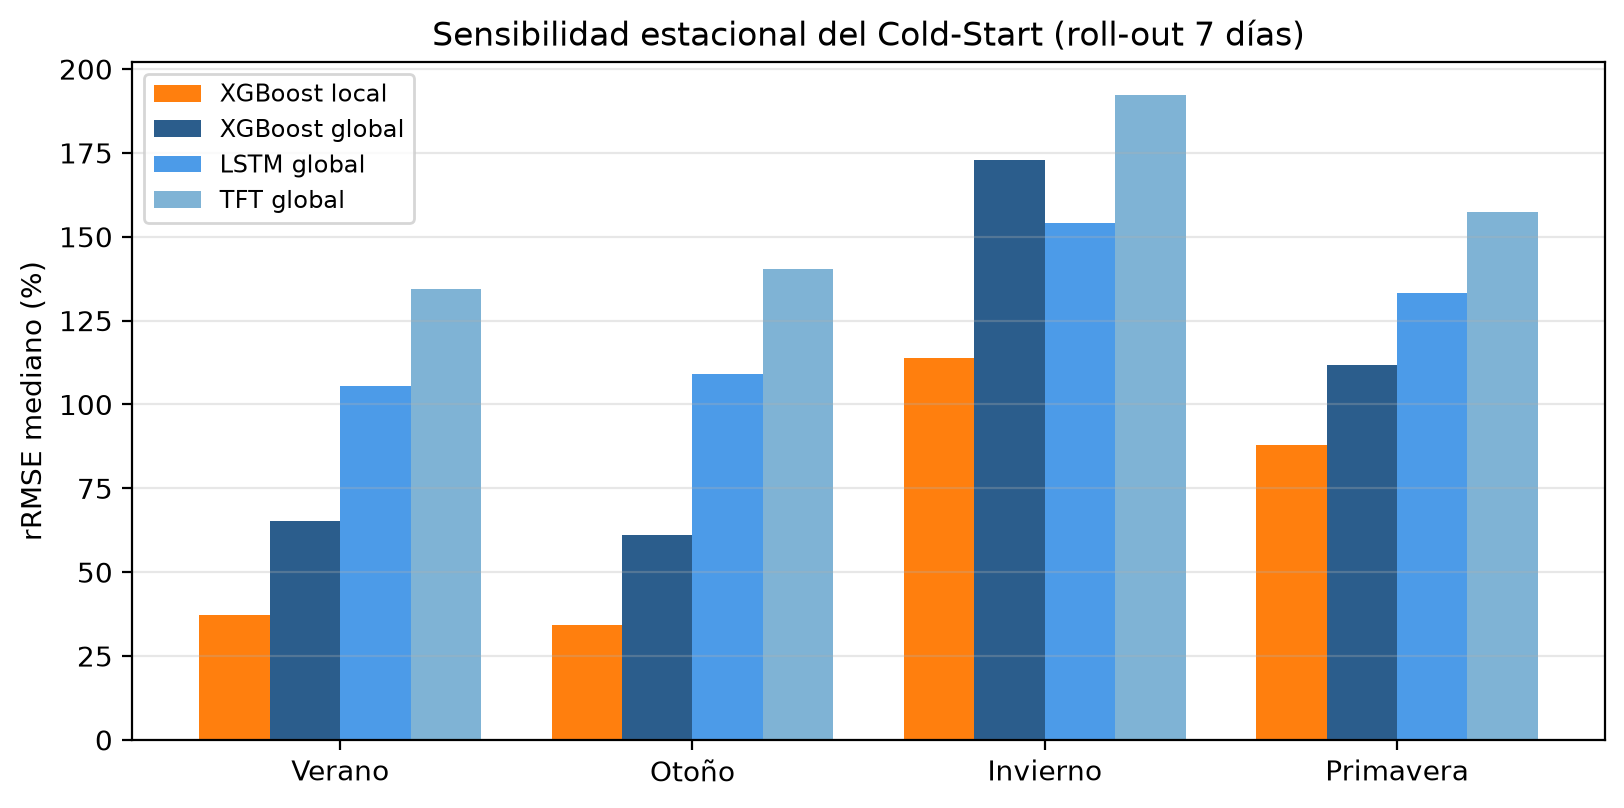
\includegraphics[width=\linewidth]{fig_estacional.png}
    \end{column}
    \begin{column}{0.5\textwidth}
      \textbf{rRMSE roll-out por estación}
      \vspace{0.3em}

      \begin{itemize}
        \item XGBoost global: \; 52\,\% (verano) $\rightarrow$ \rj{134\,\%} (invierno)
        \item XGBoost local: \; 40\,\% $\rightarrow$ \rj{115\,\%}
      \end{itemize}
      \vspace{0.5em}
      Mayor variabilidad nubosa y menor irradiación invernal debilitan la señal determinista del perfil solar.
      \vspace{0.5em}

      \textbf{Implicación operativa:} la incertidumbre de un parque nuevo depende fuertemente de la \textbf{estación de su puesta en marcha}.
    \end{column}
  \end{columns}
\end{frame}

\begin{frame}{Calidad probabilística: la calibración no se transfiere}
  \small
  \begin{center}
  \begin{tabular}{llcc}
    \toprule
    Config. & Tipo & Cobertura diurna & Pinball P95 (MWh) \\
    \midrule
    XGBoost  & \lo{Local}  & \textbf{0,86} & \textbf{0,035} \\
    XGBoost  & \gl{Global} & 0,97 (sobre-cubre) & 0,092 \\
    LSTM     & \gl{Global} & 0,53 & 0,159 \\
    Informer & \gl{Global} & 0,64 & 0,115 \\
    TFT      & \gl{Global} & 0,38 & 0,158 \\
    N-HiTS   & \gl{Global} & 0,37 & 0,372 \\
    \bottomrule
  \end{tabular}
  \end{center}
  \normalsize
  \begin{itemize}
    \item Nominal = 0,90. \textbf{Ningún paradigma calibra idealmente}, con desvíos opuestos.
    \item Redes globales \rj{subcalibradas} (bandas demasiado estrechas); XGBoost global \rj{sobre-cubre}.
    \item \lo{XGBoost local} es el más cercano al nominal y con menor pinball.
  \end{itemize}
\end{frame}

\begin{frame}{Contraste de la hipótesis --- con test estadístico}
  % OJO: dentro de un título de bloque NO usar \rj/\lo/\gl — el fondo ya es de color
  % y el texto quedaría invisible (rojo sobre rojo). Se usa negrita sobre el blanco heredado.
  \begin{alertblock}{La hipótesis se \textbf{RECHAZA}, y ahora con significancia}
    \lo{XGBoost local} gana a \gl{XGBoost global} en \textbf{77 de 94 plantas}
    ($p<10^{-7}$, Wilcoxon pareado con corrección de Holm).
  \end{alertblock}
  \begin{block}{A igualdad de arquitectura: ningún global gana significativamente}
    \begin{itemize}
      \item \lo{N-HiTS local} supera a \gl{N-HiTS global} en \textbf{88/94} ($p<10^{-10}$).
      \item El par \textbf{LSTM} es un \rj{empate estadístico}: 49/45 plantas, $p=1{,}00$.
            El matiz que sugerían las medianas \textbf{no sobrevive} al test pareado.
    \end{itemize}
  \end{block}
  \begin{exampleblock}{El valor real: disponibilidad inmediata}
    En el arranque en frío puro (historia local nula) el modelo global \textbf{no tiene competidor local posible}.
  \end{exampleblock}
\end{frame}

\begin{frame}{Ejemplo de roll-out Cold-Start a 7 días}
  \centering
  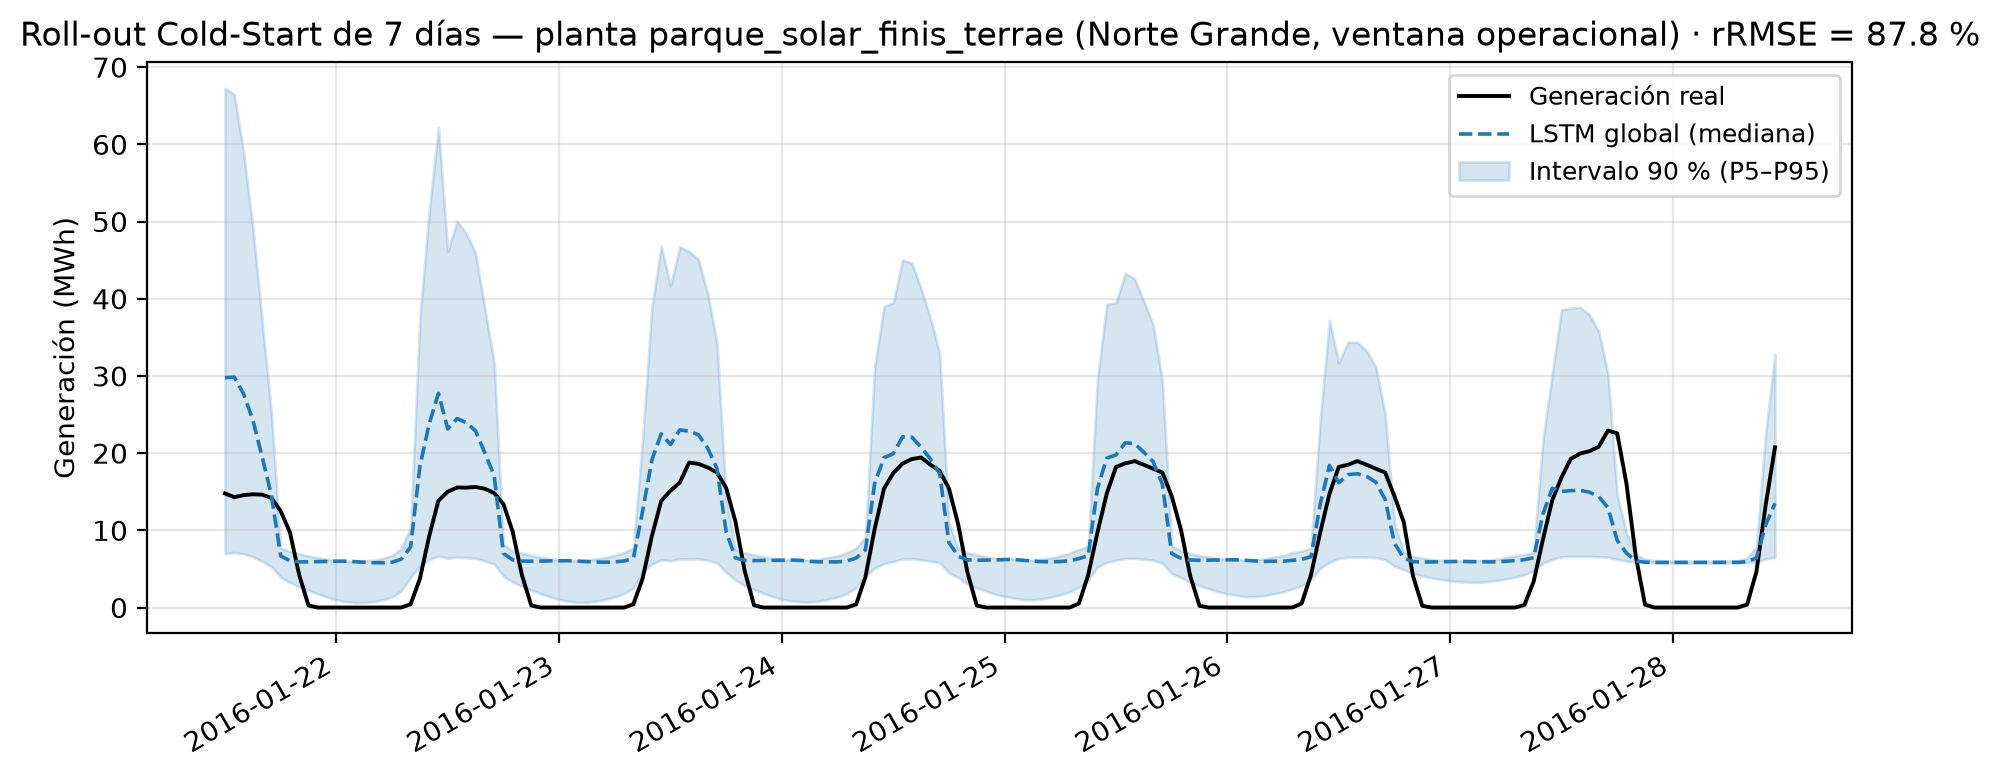
\includegraphics[width=0.9\textwidth]{fig_ejemplo_rollout.png}

  {\footnotesize El modelo global, \textbf{sin haber visto jamás la planta}, reproduce el ciclo diario y la magnitud de los picos usando solo el clima entrante y la geografía estática.}
\end{frame}

% ==================================================================
\section{Conclusiones}
% ==================================================================

\begin{frame}{Conclusiones}
  \begin{enumerate}
    \item \textbf{Resultado negativo riguroso:} bajo un protocolo estrictamente ciego, un XGBoost local maduro sigue siendo el estándar a batir. La hipótesis se rechaza.
    \item \textbf{El paradigma global conserva un régimen propio:} el arranque en frío puro, donde entrega pronósticos coherentes y accionables desde la hora cero.
    \item Cuatro hallazgos metodológicos transferibles:
    \begin{itemize}
      \item las rampas de puesta en marcha distorsionan las métricas (análisis Raw/Operacional);
      \item el invierno es sistemáticamente la estación más difícil;
      \item la calibración probabilística no se transfiere a las redes profundas;
      \item la integridad del \emph{target} (nunca imputar $y$) es esencial para la honestidad de las métricas.
    \end{itemize}
  \end{enumerate}
\end{frame}

\begin{frame}{Trabajo futuro}
  \begin{itemize}
    \item \textbf{Fine-tuning en dos etapas:} pre-entrenar global $\rightarrow$ ajustar con los primeros días reales; cierra la brecha con el local a medida que crece la historia.
    \item \textbf{Máscaras de intermitencia} en la atención: excluir la noche determinista y concentrar capacidad en la señal productiva.
    \item \textbf{Recalibración conformal} de los intervalos bajo transferencia.
    \item \textbf{Más datos y cómputo:} ampliar el corpus y el presupuesto de pasos (posible sub-entrenamiento de TFT/Informer en 6\,GB).
    \item \textbf{Máscara astronómica} para el forzamiento nocturno independiente de sensores.
  \end{itemize}
\end{frame}

\begin{frame}[plain]
  \centering
  \vfill
  {\usebeamercolor[fg]{structure}\Huge \textbf{Gracias}}\\[0.5em]
  {\Large ¿Preguntas?}\\[1.0em]
  
\includegraphics[width=0.13\linewidth]{figuras/logoUCM.png}\\[0.5em]
  \ifnum\confmode=1
    {\normalsize César David Aular Muñoz \quad·\quad Sergio Hernández}\\
    {\footnotesize cesaraular02@gmail.com \quad·\quad Universidad Católica del Maule}
  \else
    {\normalsize César David Aular Muñoz}\\
    {\footnotesize cesaraular02@gmail.com}
  \fi
  \vfill
\end{frame}

% ==================================================================
% BACKUP SLIDES — anticipando los ataques de la comisión
% ==================================================================
\appendix

\begin{frame}{Backup --- Tests estadísticos (Friedman + Wilcoxon-Holm)}
  \textbf{Diseño pareado y balanceado:} 94 plantas $\times$ 8 configuraciones sobre la
  misma grilla horaria canónica $\rightarrow$ aplica la comparación por rangos de
  Demšar (2006).
  \vspace{0.3em}
  \begin{itemize}
    \item \textbf{Friedman (omnibus):} $\chi^2 = 260{,}7$, $p < 10^{-50}$ — las
          configuraciones no son equivalentes.
    \item \textbf{Ranking medio} (1 = mejor): XGB local 1,80 · N-HiTS local 3,32 ·
          XGB global 3,34 · TFT 5,10 · Informer 5,15 · LSTM local 5,30 ·
          LSTM global 5,41 · N-HiTS global 6,59.
    \item \textbf{Mejor por planta:} XGB local en 60/94, XGB global en 15,
          N-HiTS local en 10.
  \end{itemize}
  \vspace{0.2em}
  \begin{alertblock}{Por qué la mediana marginal engañaba}
    rRMSE mediano sugería \gl{LSTM global} (118\,\%) mejor que \lo{LSTM local}
    (147\,\%). Pero la \textbf{mediana de las diferencias por planta} es $\approx 0$ y
    levemente a favor del local: la brecha la producían unas pocas plantas donde el
    local falla mucho, no una ventaja sistemática del global.
  \end{alertblock}
\end{frame}

\begin{frame}{Backup --- Causalidad temporal de los baselines locales}
  \begin{block}{Qué se hizo exactamente}
    Los baselines locales se entrenan con la historia \textbf{completa} de la planta
    \textbf{menos todas las ventanas de evaluación} (Raw, Operacional y las 4
    estacionales), con los \emph{lags} hacia esas ventanas enmascarados.
  \end{block}
  \begin{itemize}
    \item No hay fuga del \emph{target}: ningún rezago apunta dentro de una ventana.
    \item Pero el entrenamiento \textbf{sí incluye horas posteriores} a la ventana
          predicha $\rightarrow$ \rj{no es estrictamente causal}.
    \item Es una elección de diseño: representa el modelo maduro que el operador
          tendría \emph{tras acumular historia} — el rival más fuerte posible.
  \end{itemize}
  \begin{exampleblock}{Por qué esto refuerza la conclusión}
    El sesgo favorece al lado \lo{local}, que \textbf{gana}; y el espejo (LOPO oculta
    la planta pero \textbf{no el calendario}) favorece al lado \gl{global}, que
    \textbf{pierde igual}. Ambos sesgos empujan contra la conclusión reportada.
  \end{exampleblock}
\end{frame}

\begin{frame}{Backup --- Definición del RMSE}
  \begin{block}{Fórmula}
    \[
      \mathrm{RMSE} = \sqrt{\frac{1}{n}\sum_{i=1}^{n}\left(y_i - \hat{y}_i\right)^2}
    \]
  \end{block}
  \begin{itemize}
    \item Eleva al \textbf{cuadrado} cada error antes de promediar $\rightarrow$ penaliza las desviaciones grandes de forma \rj{cuadrática}, no lineal ni logarítmica.
    \item Ideal para el pronóstico FV: castiga con fuerza los errores en los \textbf{picos de inyección} de mediodía.
    \item Comparte unidades con la variable (MWh), a diferencia del MSE.
    \item \textbf{rRMSE} = RMSE normalizado por la generación media horaria de la ventana (ver backup siguiente).
  \end{itemize}
\end{frame}

\begin{frame}{Backup --- ¿Por qué el rRMSE supera el 100\,\%?}
  \[
    \mathrm{rRMSE} = \frac{\mathrm{RMSE}}{\overline{y}_{\text{ventana}}}\times 100
  \]
  \begin{itemize}
    \item El denominador $\overline{y}$ incluye las \textbf{horas nocturnas de generación nula}.
    \item Esto \textbf{deprime la media} y por tanto \textbf{infla} sistemáticamente el indicador.
    \item Valores $>100\,\%$ son \textbf{esperables} en pronóstico horario FV bajo esta normalización.
    \item Su valor no es la magnitud absoluta, sino la \rj{comparación relativa} entre arquitecturas sobre \textbf{ventanas idénticas}.
  \end{itemize}
  \vspace{0.3em}
  \centering\footnotesize
  Todas las configuraciones se comparan sobre la misma grilla horaria canónica $\rightarrow$ comparación estrictamente pareada.
\end{frame}

\begin{frame}{Backup --- Calibración de XGBoost (global vs.\ local)}
  \begin{columns}[T]
    \begin{column}{0.5\textwidth}
      \textbf{XGBoost global: 0,97 (sobre-cubre)}
      \begin{itemize}
        \item Regresión cuantílica sobre un contexto \textbf{heterogéneo} ($N-1$ plantas).
        \item Bandas \textbf{demasiado anchas}: casi nunca fallan, pero pierden utilidad operativa.
        \item Un defecto \textbf{simétrico} al de las redes, no una virtud.
      \end{itemize}
    \end{column}
    \begin{column}{0.5\textwidth}
      \textbf{XGBoost local: 0,86 (casi nominal)}
      \begin{itemize}
        \item Ajustado a la variabilidad \textbf{real} de la propia planta.
        \item Pinball P95 = \textbf{0,035} MWh vs.\ 0,092 del global.
        \item Intervalos más estrechos y \textbf{mejor centrados}.
      \end{itemize}
    \end{column}
  \end{columns}
  \vspace{0.5em}
  \begin{alertblock}{¿Por qué las redes profundas subcalibran?}
    Su escalador local se ajusta sobre el \textbf{contexto sintético}, cuya varianza (perfil solar idealizado) es menor que la real $\rightarrow$ bandas estrechas. Los baselines locales profundos, con contexto real, mejoran (LSTM local 0,79).
  \end{alertblock}
\end{frame}

\begin{frame}{Backup --- Detalles de cómputo}
  \begin{itemize}
    \item \textbf{Precisión fp32} completa: la mezcla fp16 introducía inestabilidad numérica en el entrenamiento.
    \item \textbf{GPU RTX 2060 (6\,GB):} la VRAM la gobierna \texttt{batch\_size}$\times$\texttt{windows\_batch\_size}, no el tamaño del corpus $\rightarrow$ no se trunca la historia.
    \item \textbf{Presupuesto por época corregido:} cada paso consume \texttt{batch}$\times$\texttt{windows\_batch} ventanas; la fórmula ingenua \texttt{filas/batch} sobreestimaba $\sim$250$\times$.
    \item \textbf{\emph{Early stopping}} sobre \texttt{val\_size}=168; tuning cacheado una vez por modelo y reusado entre folds (fuga a nivel de hiperparámetro: despreciable y documentada).
    \item Toda predicción se fuerza a $\hat{y}\geq 0$ y a cero de noche (consistencia física).
  \end{itemize}
\end{frame}

\begin{frame}{Backup --- Tabla completa (day1 y roll-out)}
  \scriptsize
  \begin{center}
  \begin{tabular}{llcccccc}
    \toprule
     & & \multicolumn{2}{c}{NRMSE (\% cap.)} & \multicolumn{2}{c}{rRMSE (\%)} & & \\
    \cmidrule(lr){3-4}\cmidrule(lr){5-6}
    Config. & Tipo & day1 & roll7d & day1 & roll7d & Cob. & Pinball \\
    \midrule
    XGBoost  & \lo{Local}  & \textbf{9,5} & \textbf{13,2} & 45,6 & 59,9 & 0,86 & 0,035 \\
    XGBoost  & \gl{Global} & 15,6 & 17,1 & 64,0 & 75,1 & 0,97 & 0,092 \\
    N-HiTS   & \lo{Local}  & 14,2 & 17,6 & 62,3 & 85,2 & 0,72 & 0,096 \\
    Informer & \gl{Global} & 21,0 & 22,8 & 96,6 & 106,5 & 0,64 & 0,115 \\
    TFT      & \gl{Global} & 22,0 & 23,6 & 105,1 & 112,7 & 0,38 & 0,158 \\
    LSTM     & \lo{Local}  & 16,3 & 23,9 & 102,6 & 128,8 & 0,72 & 0,235 \\
    LSTM     & \gl{Global} & 22,6 & 24,8 & 99,7 & 108,6 & 0,53 & 0,159 \\
    N-HiTS   & \gl{Global} & 28,6 & 30,7 & 129,8 & 148,2 & 0,37 & 0,372 \\
    \bottomrule
  \end{tabular}
  \end{center}
  \normalsize
  \centering Ventana \emph{cold-start}, mediana sobre las \textbf{94 plantas}
  (Operacional donde hay rampa $>$24\,h; Raw en el resto).
\end{frame}

\end{document}
"
% Solo cambian portada/autores/afiliacion/evento; el contenido es el mismo.
% ====================================================================
\providecommand{\confmode}{0}% 0 = defensa, 1 = conferencia
\usepackage[utf8]{inputenc}
\usepackage[T1]{fontenc}
\usepackage[spanish,es-noquoting]{babel}
% Evita el "Incompatible glue units" de babel-spanish al usar \% dentro de beamer
\makeatletter
\let\es@sppercent\relax
\makeatother
\usepackage{graphicx}
\usepackage{booktabs}
\usepackage{amsmath}
\usepackage{xcolor}

\graphicspath{{figuras/}}

% --- Metadatos (usados por la plantilla oficial en portada, pie y cabecera) ---
\ifnum\confmode=1
  % ----- Modo CONFERENCIA (paper IEEE) -----
  \title[Pronóstico FV \emph{Cold-Start} · LOPO]{Pronóstico fotovoltaico a corto plazo bajo escasez de datos mediante evaluación \emph{Leave-One-Plant-Out}}
  \subtitle{Un enfoque \emph{Cross-Site} multi-planta frente a modelos locales}
  \author[Aular \& Hernández]{César David Aular Muñoz \and Sergio Hernández}
  \institute[UCM]{Departamento de Computación e Industrias \\ Facultad de Ciencias de la Ingeniería \\ Universidad Católica del Maule}
  \date{Chilean Workshop on Pattern Recognition (CWPR) --- 2026}
\else
  % ----- Modo DEFENSA (examen de título) -----
  \title[Multi-sitio vs.\ local: pronóstico FV \emph{Cold-Start}]{Análisis comparativo de un enfoque multi-sitio frente a modelos locales para la proyección a corto plazo de generación fotovoltaica bajo escasez de datos}
  % \subtitle{Proyección a corto plazo de generación fotovoltaica bajo escasez de datos}
  \author[César Aular]{César David Aular Muñoz}
  \institute[Escuela ICI --- UCM]{Escuela Ingeniería Civil Informática \\ Universidad Católica del Maule}
  \date{Proyecto de Título --- Junio 2026}
\fi

% --- Plantilla oficial de presentación UCM (tema QUT: azul institucional #00407a) ---
\usepackage{QUT}

% --- Colores semánticos: global (azul) / local (verde) / alerta (rojo) ---
\definecolor{glob}{HTML}{1F77B4}
\definecolor{loc}{HTML}{2CA02C}
\definecolor{alertred}{HTML}{C0392B}
\newcommand{\gl}[1]{\textcolor{glob}{\textbf{#1}}}
\newcommand{\lo}[1]{\textcolor{loc}{\textbf{#1}}}
\newcommand{\rj}[1]{\textcolor{alertred}{\textbf{#1}}}

% --- Bloques redondeados con relleno (info=azul UCM / ejemplo=verde / alerta=rojo) ---
\setbeamertemplate{blocks}[rounded][shadow=true]
\setbeamercolor{block title}{bg=qut,fg=white}
\setbeamercolor{block body}{bg=qut!8,fg=black}
\setbeamercolor{block title example}{bg=loc,fg=white}
\setbeamercolor{block body example}{bg=loc!8,fg=black}
\setbeamercolor{block title alerted}{bg=alertred,fg=white}
\setbeamercolor{block body alerted}{bg=alertred!8,fg=black}

\begin{document}

\begin{frame}[plain]
  \titlepage
  \begin{center}
    
\includegraphics[width=0.16\linewidth]{figuras/logoUCM.png}
  \end{center}
\end{frame}

\begin{frame}{Agenda}
  \tableofcontents[hideallsubsections]
\end{frame}

% ==================================================================
\section{El problema}
% ==================================================================

\begin{frame}{El problema del \emph{Cold-Start} fotovoltaico}
  \begin{columns}[T]
    \begin{column}{0.56\textwidth}
      \begin{itemize}
        \item Una planta FV \textbf{recién conectada} no tiene historial de generación.
        \item Los modelos clásicos entrenan \textbf{uno por planta} con meses o años de datos locales.
        \item Aplicados a una planta nueva: \rj{no se pueden entrenar} o se degradan gravemente.
      \end{itemize}
      \vspace{0.4em}
      \begin{alertblock}{Consecuencia}
        Incertidumbre justo cuando más se necesita certeza $\rightarrow$ mayores costos de balance y riesgo financiero, en especial para los pequeños PMGD.
      \end{alertblock}
    \end{column}
    \begin{column}{0.44\textwidth}
      \centering
      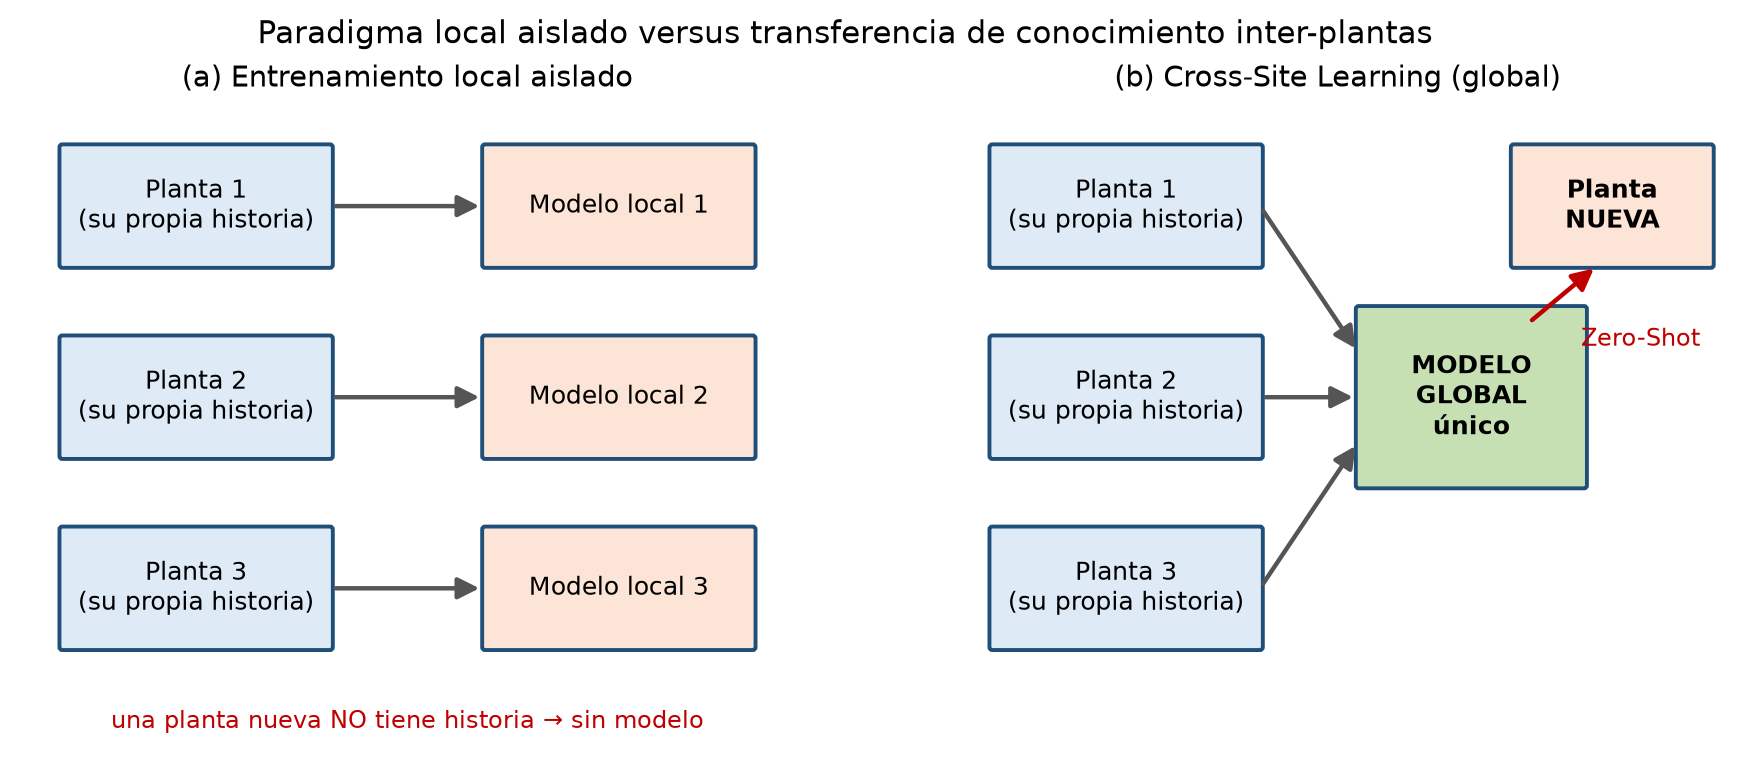
\includegraphics[width=\linewidth]{fig_cross_site.png}
      \vspace{0.3em}

      {\footnotesize El problema del arranque en frío, tomado de los sistemas de recomendación.}
    \end{column}
  \end{columns}
\end{frame}

\begin{frame}{La idea: aprendizaje \emph{Cross-Site}}
  \begin{columns}[T]
    \begin{column}{0.5\textwidth}
      Abandonar el supuesto \textbf{un-modelo-por-planta}.

      \vspace{0.6em}
      Un único modelo \gl{global} entrenado sobre \textbf{muchas plantas a la vez}:
      \begin{itemize}
        \item absorbe patrones compartidos clima~$\rightarrow$~potencia,
        \item los \textbf{transfiere} a una planta jamás vista,
        \item pronostica \textbf{desde la primera hora} de conexión.
      \end{itemize}
      \vspace{0.5em}
      \textbf{Pregunta central (adversarial):}\\
      \emph{¿realmente supera a una línea base local madura, o el premio de la transferencia se desvanece con una comparación justa?}
    \end{column}
    \begin{column}{0.5\textwidth}
      \centering
      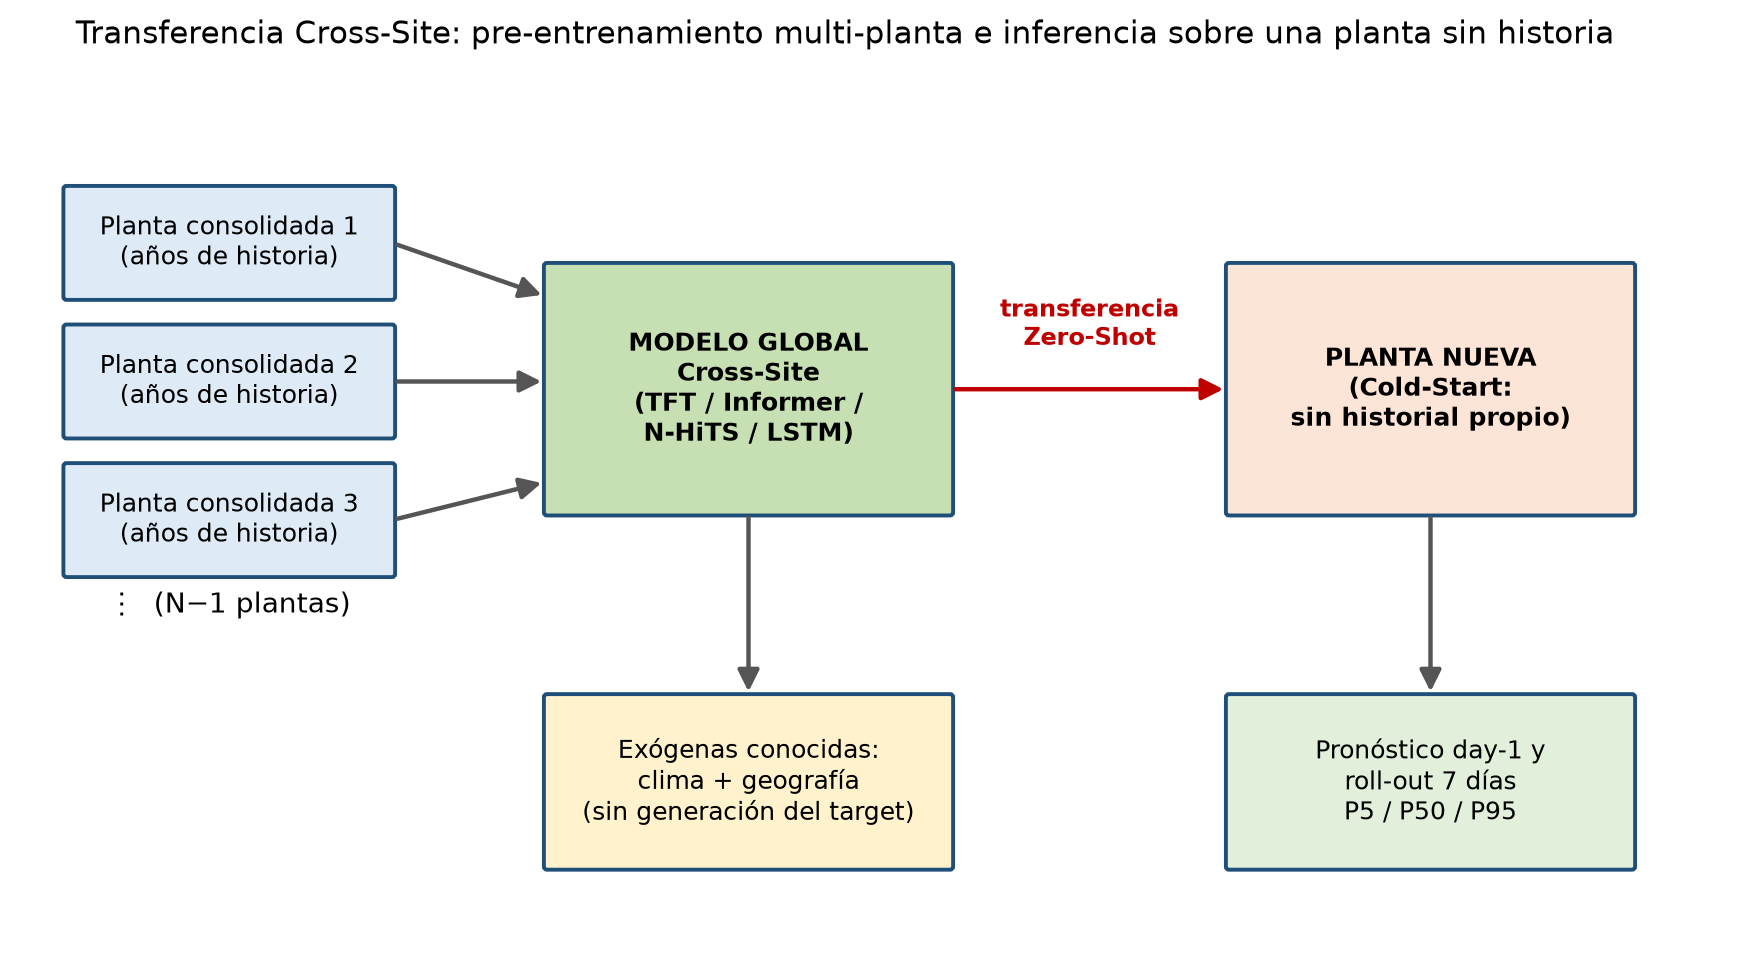
\includegraphics[width=\linewidth]{fig_solucion.png}
    \end{column}
  \end{columns}
\end{frame}

\begin{frame}{Hipótesis y objetivos}
  \begin{block}{Hipótesis}
    El modelo global multi-sitio es \emph{más preciso} que un modelo entrenado localmente con la historia propia del centro.
  \end{block}
  \begin{columns}[T]
    \begin{column}{0.5\textwidth}
      \textbf{Objetivos específicos}
      \begin{enumerate}
        \item Adaptar una arquitectura Transformer al entrenamiento multi-serie.
        \item Evaluarla frente a modelos locales bajo un protocolo \emph{Cold-Start} estricto.
        \item Integrar datos multimodales sin fuga de información.
      \end{enumerate}
    \end{column}
    \begin{column}{0.5\textwidth}
      \textbf{La brecha en la literatura}\\
      Rara vez se combinan a la vez:
      \begin{enumerate}
        \item evaluación \textbf{ciega} a la planta objetivo (sin \emph{fine-tuning}),
        \item contraste \textbf{justo} contra locales maduros,
        \item caracterización \textbf{probabilística}.
      \end{enumerate}
    \end{column}
  \end{columns}
\end{frame}

% ==================================================================
\section{Metodología}
% ==================================================================

\begin{frame}{Arquitectura del sistema}
  \centering
  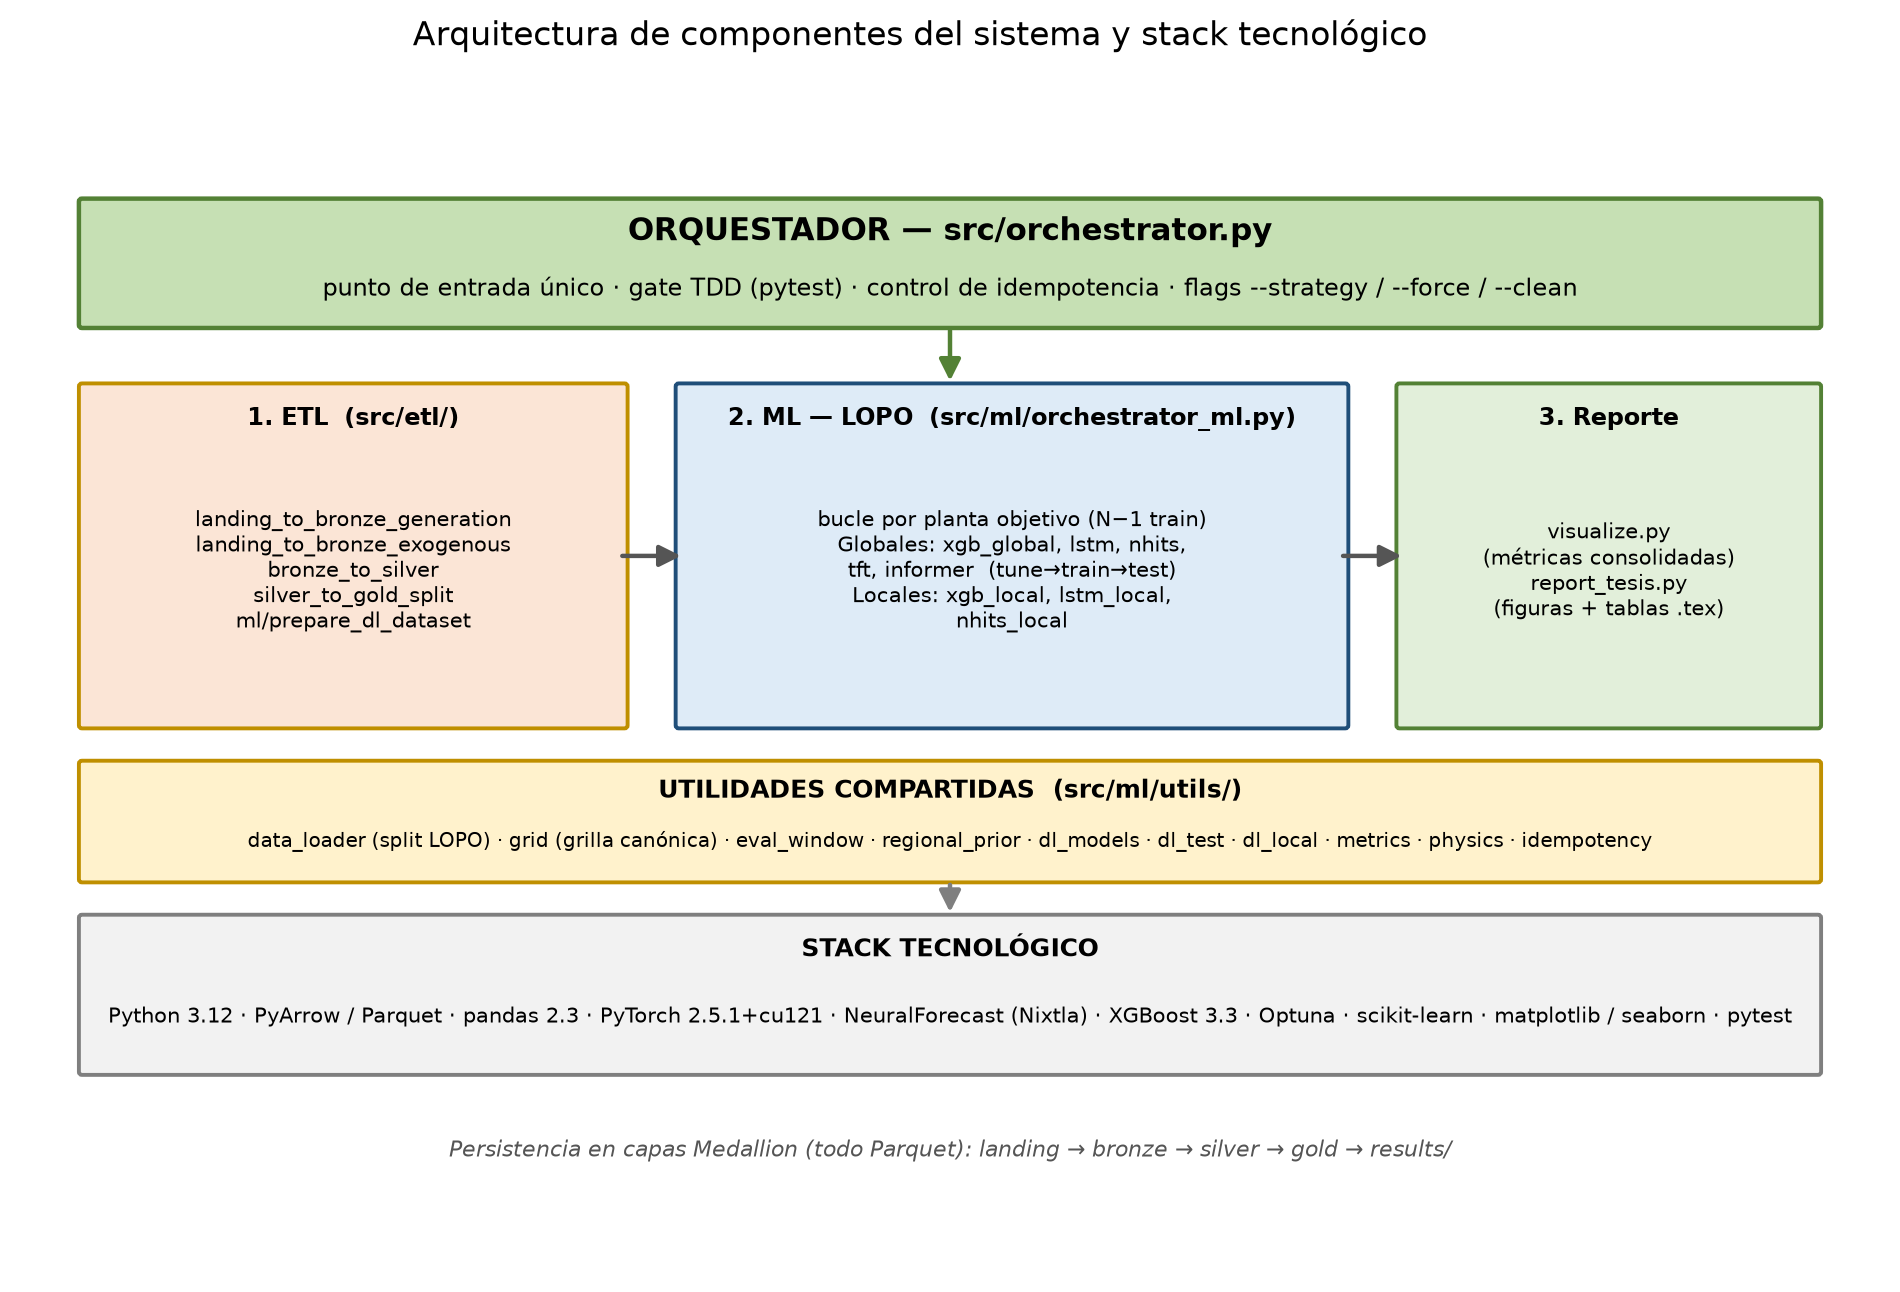
\includegraphics[height=0.78\textheight,keepaspectratio]{fig_arquitectura_componentes.png}
\end{frame}

\begin{frame}{Protocolo \emph{Leave-One-Plant-Out} (LOPO)}
  \begin{columns}[T]
    \begin{column}{0.52\textwidth}
      \begin{itemize}
        \item Para cada planta objetivo: los globales entrenan con las \textbf{$N-1$ restantes} (2014--2024 completo).
        \item La planta objetivo es \rj{invisible} durante el entrenamiento.
        \item Métricas: \textbf{mediana} sobre 94 plantas, solo observaciones reales.
      \end{itemize}
      \begin{exampleblock}{Integridad Zero-Shot (no negociable)}
        Ninguna variable puede ser función de la generación del objetivo. Verificado por pruebas automatizadas.
      \end{exampleblock}
    \end{column}
    \begin{column}{0.48\textwidth}
      \centering
      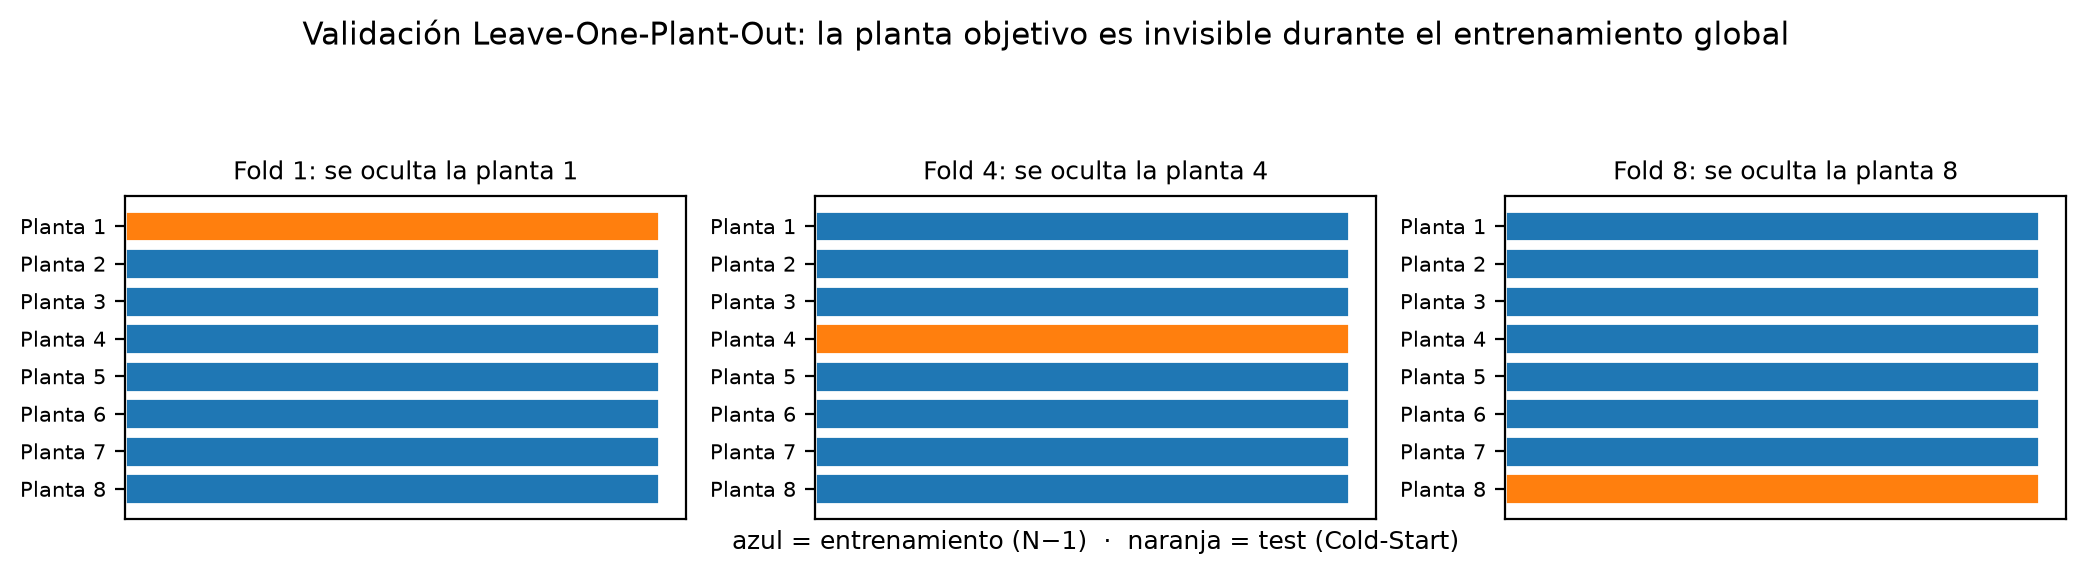
\includegraphics[width=\linewidth]{fig_lopo.png}
    \end{column}
  \end{columns}
\end{frame}

\begin{frame}{La lección de la fuga de datos}
  \begin{center}
    \Large Un \emph{prior} de eficiencia calculado \textbf{por-fila} desde el objetivo
  \end{center}
  \vspace{0.3em}
  \[
    PR = \frac{y}{\text{capacidad}} \quad\Longrightarrow\quad \mathrm{corr}(PR,\,y)=1.0
  \]
  \vspace{0.2em}
  \begin{columns}[T]
    \begin{column}{0.5\textwidth}
      \begin{alertblock}{rRMSE falso}
        $\approx 0.8\,\%$ \; (demasiado bueno para ser verdad)
      \end{alertblock}
    \end{column}
    \begin{column}{0.5\textwidth}
      \begin{exampleblock}{rRMSE honesto (tras corregir)}
        $\approx 56\,\%$
      \end{exampleblock}
    \end{column}
  \end{columns}
  \vspace{0.6em}
  \centering
  El \emph{prior} regional se agrega \textbf{solo sobre las plantas de entrenamiento} (por macrozona y estación).
\end{frame}

\begin{frame}{Semilla \emph{Cold-Start} sintética}
  Los modelos profundos necesitan una ventana de contexto que la planta nueva no tiene. Se siembra sintéticamente:
  \[
    \hat{y}_{\text{seed}}(t) = \text{capacidad}\cdot PR_{\text{regional}}\cdot s(t)
  \]
  \begin{itemize}
    \item $s(t)$: perfil solar determinista; $PR_{\text{regional}}$: solo plantas de entrenamiento.
    \item Solo el clima exógeno (conocido/pronosticable) y la geografía estática usan valores reales del objetivo.
    \item La generación de contexto es \rj{100\% sintética} $\rightarrow$ cero fuga.
  \end{itemize}
  \vspace{-0.4em}
  \centering
  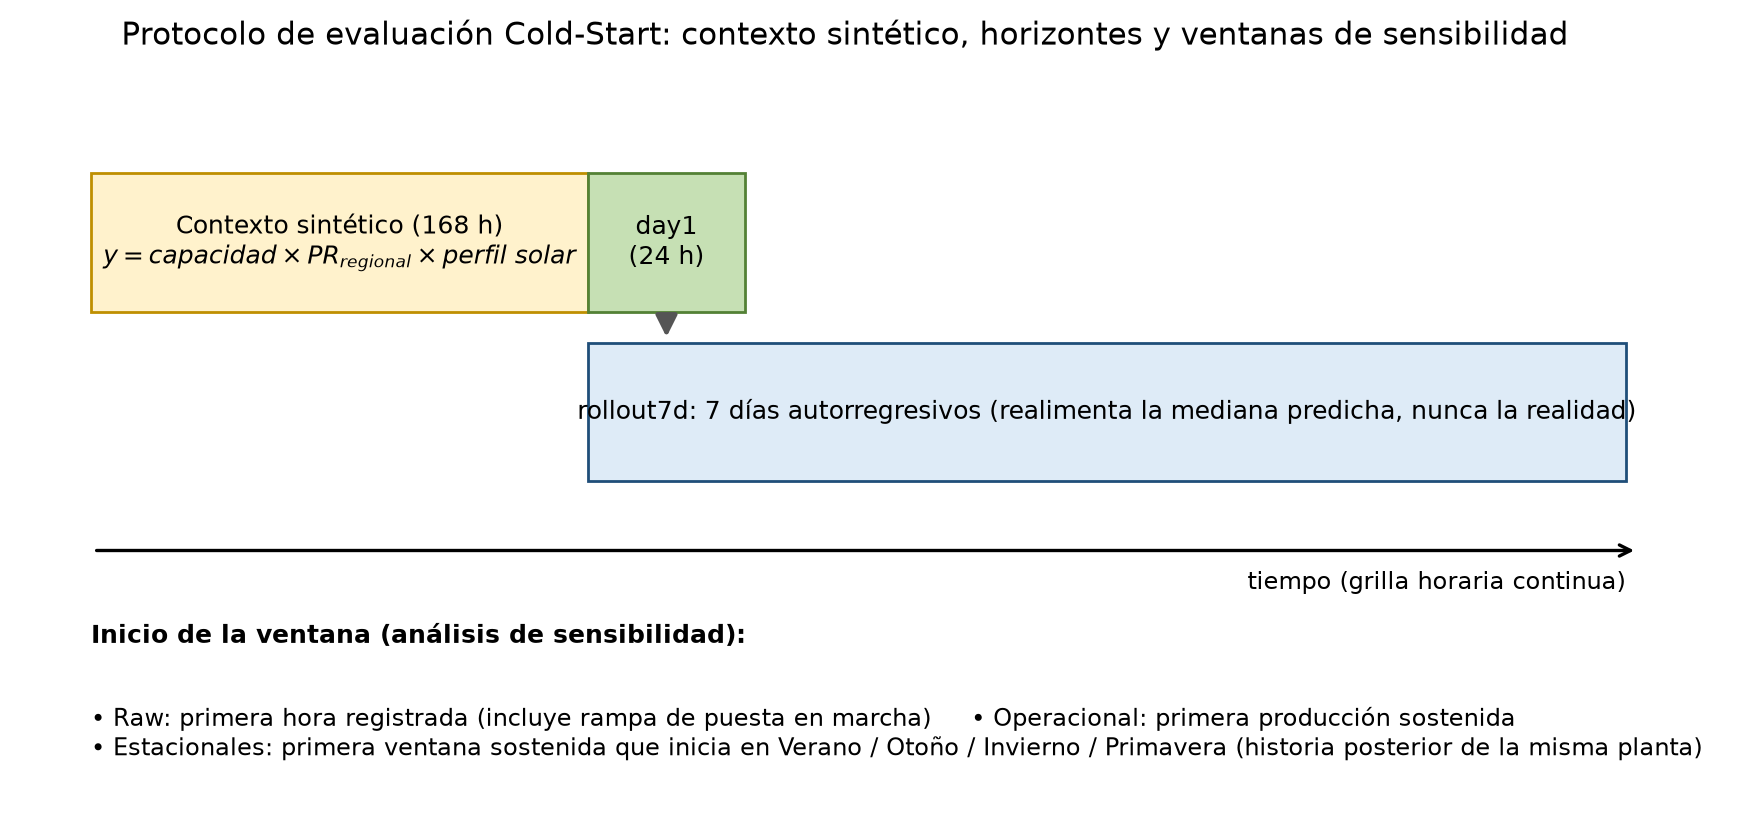
\includegraphics[width=0.54\textwidth]{fig_eval_protocolo.png}
\end{frame}

\begin{frame}{Ocho configuraciones y ventanas de evaluación}
  \begin{columns}[T]
    \begin{column}{0.48\textwidth}
      \textbf{5 globales \gl{(Cross-Site)}}
      \begin{itemize}
        \item TFT, Informer, N-HiTS, LSTM
        \item XGBoost global
      \end{itemize}
      \vspace{0.4em}
      \textbf{3 locales \lo{(estrictas)}}
      \begin{itemize}
        \item XGBoost, LSTM, N-HiTS
        \item entrenados solo con la historia propia
      \end{itemize}
      \vspace{0.5em}
      \textbf{Horizontes:} \emph{day1} (24\,h) y \emph{rollout7d} (7 días autorregresivos).
    \end{column}
    \begin{column}{0.52\textwidth}
      \centering
      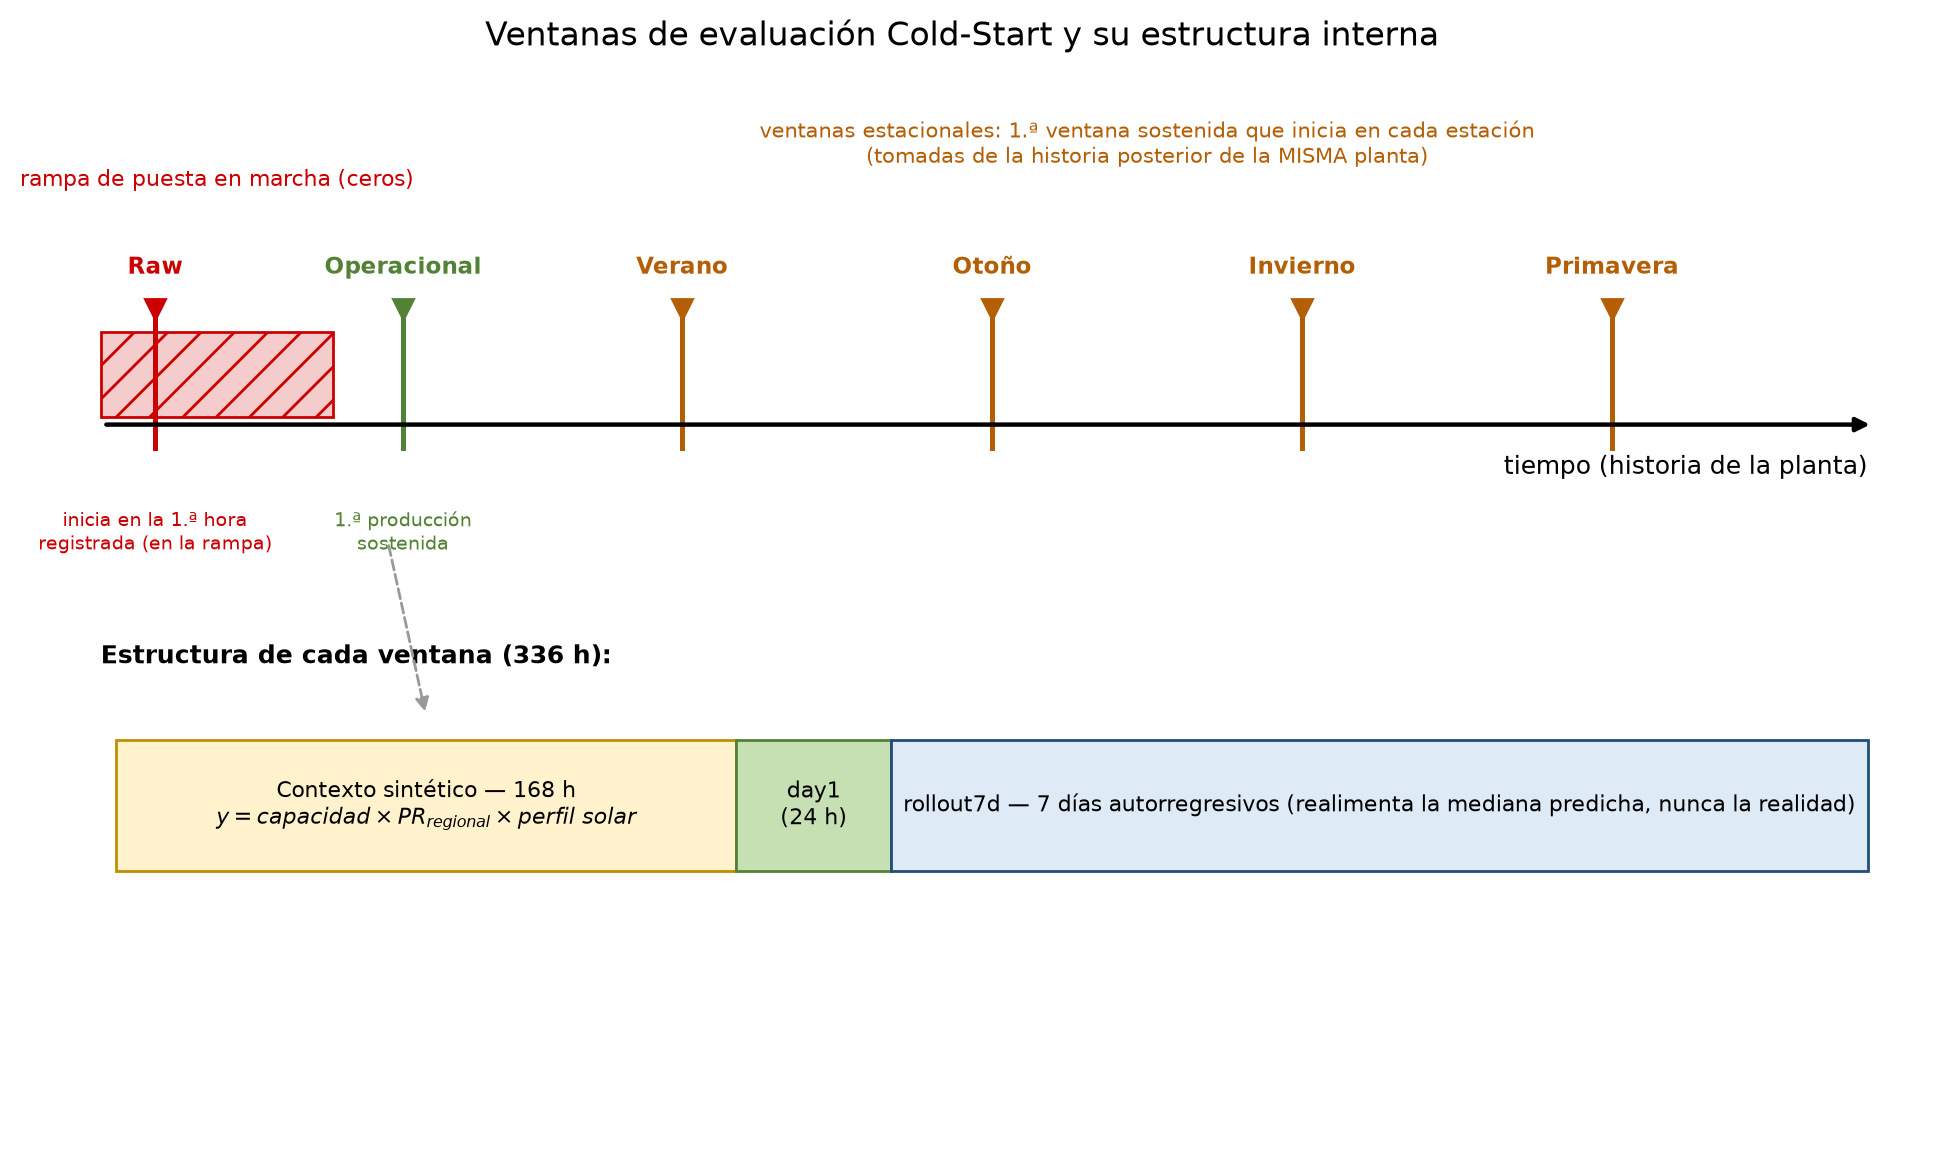
\includegraphics[width=\linewidth]{fig_ventanas_evaluacion.png}
      \vspace{0.2em}

      {\footnotesize \textbf{Raw} (incluye rampa) · \textbf{Operacional} (producción sostenida) · \textbf{Estacionales}.}
    \end{column}
  \end{columns}
\end{frame}

\begin{frame}{¿Dónde están las plantas? El corpus sobre el mapa}
  \begin{columns}[T]
    \begin{column}{0.42\textwidth}
      \centering
      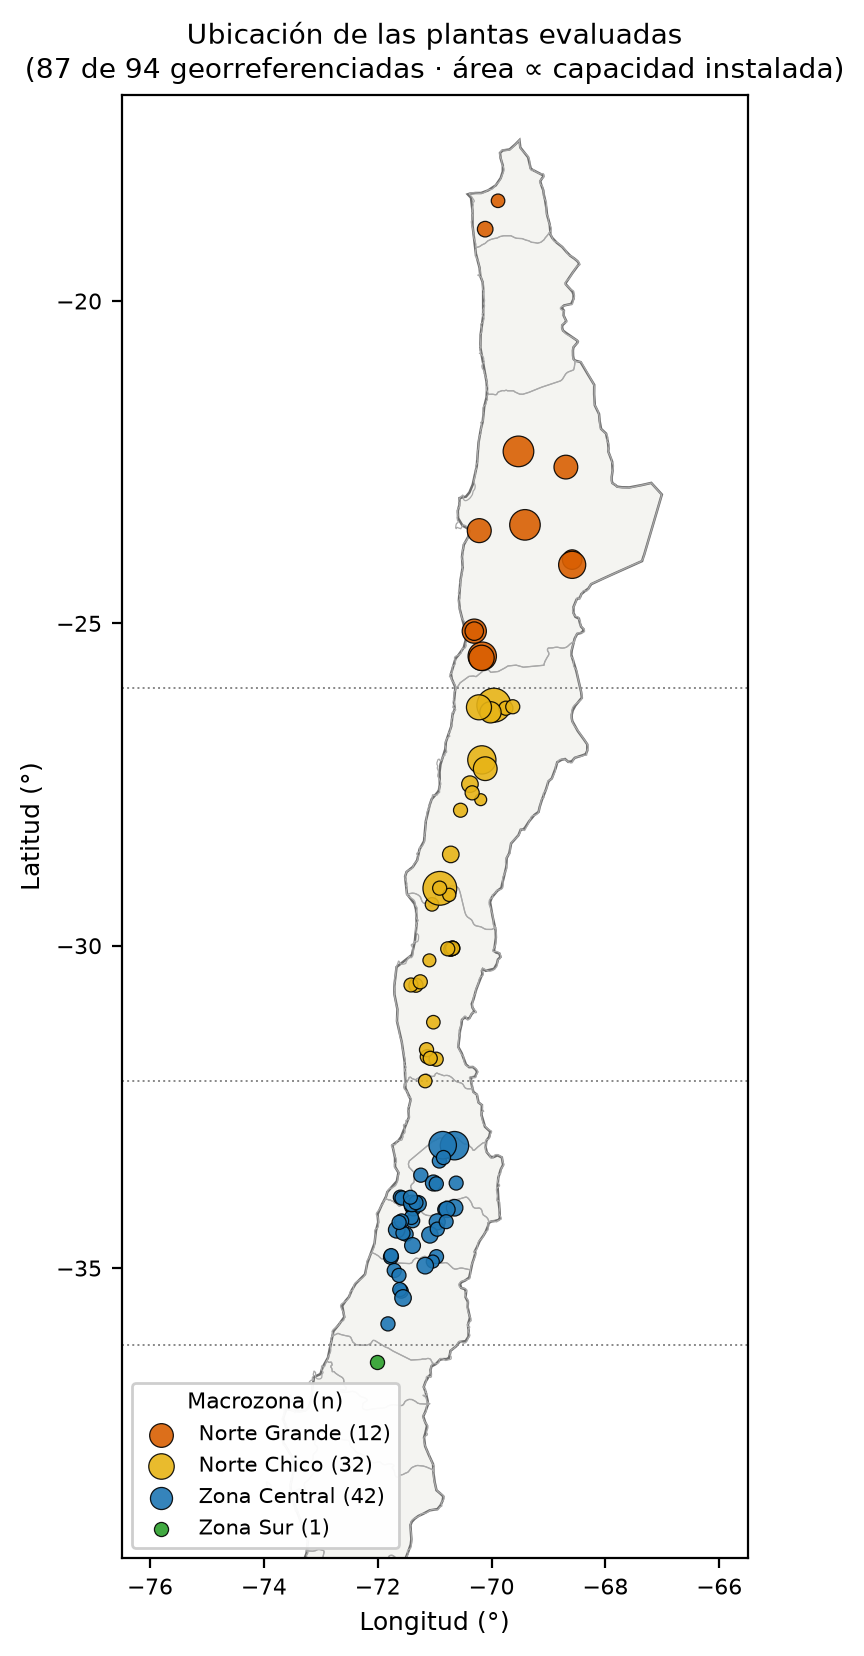
\includegraphics[height=0.78\textheight]{fig_mapa_plantas.png}
    \end{column}
    \begin{column}{0.58\textwidth}
      \vspace{1.2em}
      \begin{itemize}
        \item \textbf{94 plantas} del Sistema Eléctrico Nacional, a lo largo de todo el
              gradiente solar de Chile (Arica $\rightarrow$ zona sur).
        \item \gl{Norte Grande y Norte Chico}: pocas plantas pero \textbf{grandes}
              (utility scale, hasta 200\,MW) y de alta irradiancia.
        \item \lo{Zona Central}: muchas plantas \textbf{pequeñas} (PMGD, mediana
              $\approx$3\,MW) — el segmento que más sufre el arranque en frío.
      \end{itemize}
      \vspace{0.4em}
      \begin{exampleblock}{Por qué importa para la transferencia}
        La \textbf{macrozona} es la única señal espacial que ven los modelos, y es la
        clave sobre la que se agrega el \emph{prior} regional que siembra el contexto
        sintético.
      \end{exampleblock}
    \end{column}
  \end{columns}
\end{frame}

% ==================================================================
\section{Resultados}
% ==================================================================

\begin{frame}{Precisión puntual --- ventana \emph{cold-start}, 94 plantas (roll-out 7 días)}
  \begin{columns}[T]
    \begin{column}{0.46\textwidth}
      \small
      \begin{tabular}{llrr}
        \toprule
        Config. & Tipo & NRMSE & rRMSE \\
        \midrule
        XGBoost & \lo{Local}  & \textbf{13,2\,\%} & 60\,\% \\
        XGBoost & \gl{Global} & 17,1\,\% & 75\,\% \\
        N-HiTS  & \lo{Local}  & 17,6\,\% & 85\,\% \\
        Informer& \gl{Global} & 22,8\,\% & 107\,\% \\
        TFT     & \gl{Global} & 23,6\,\% & 113\,\% \\
        LSTM    & \lo{Local}  & 23,9\,\% & 129\,\% \\
        LSTM    & \gl{Global} & 24,8\,\% & 109\,\% \\
        N-HiTS  & \gl{Global} & 30,7\,\% & 148\,\% \\
        \bottomrule
      \end{tabular}

      \vspace{0.3em}
      {\scriptsize NRMSE = RMSE / capacidad instalada. \textbf{94 plantas}.}
    \end{column}
    \begin{column}{0.54\textwidth}
      \centering
      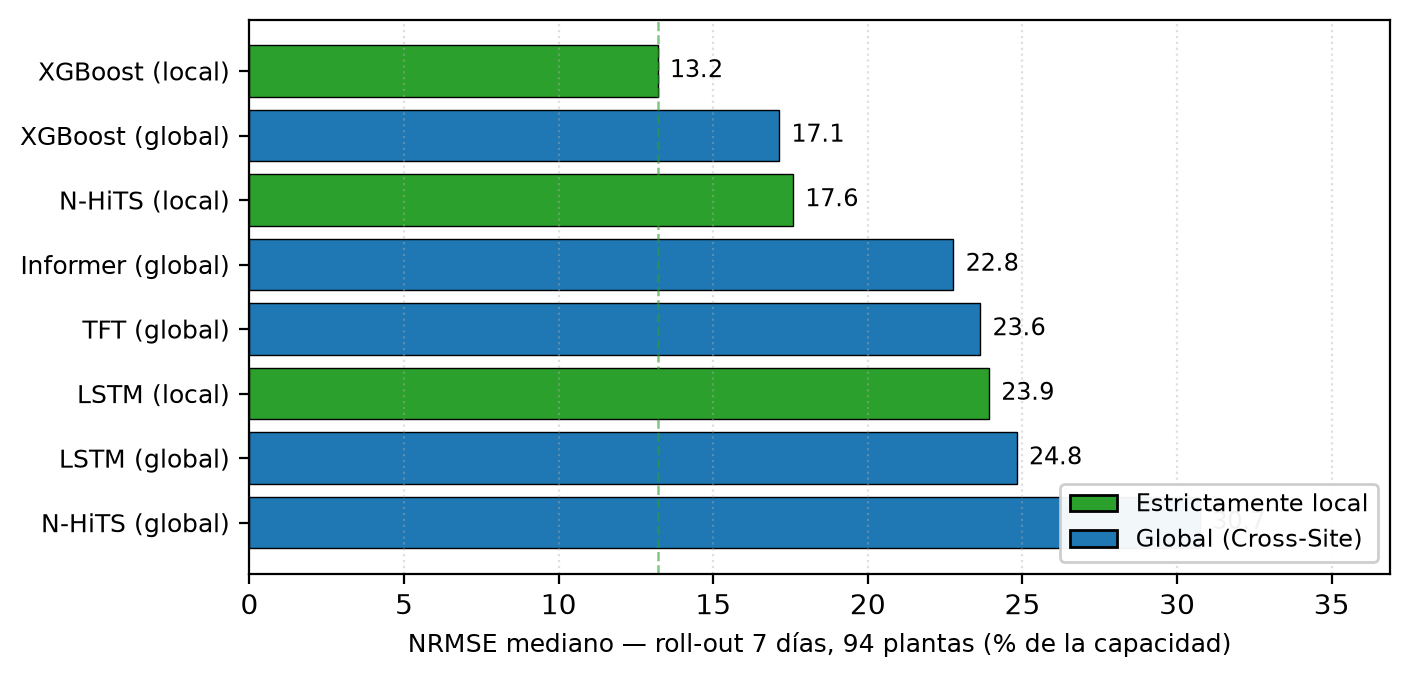
\includegraphics[width=\linewidth]{fig_resultados_nrmse_es.png}
    \end{column}
  \end{columns}
  \vspace{0.2em}
  {\footnotesize El \lo{XGBoost local} es el más preciso (13\,\% de la potencia nominal). Normalizar por \textbf{capacidad} hace los números interpretables —y cambia el orden del par LSTM respecto de rRMSE.}
\end{frame}

\begin{frame}{Sensibilidad estacional: el invierno es el gran desafío}
  \begin{columns}[T]
    \begin{column}{0.5\textwidth}
      \centering
      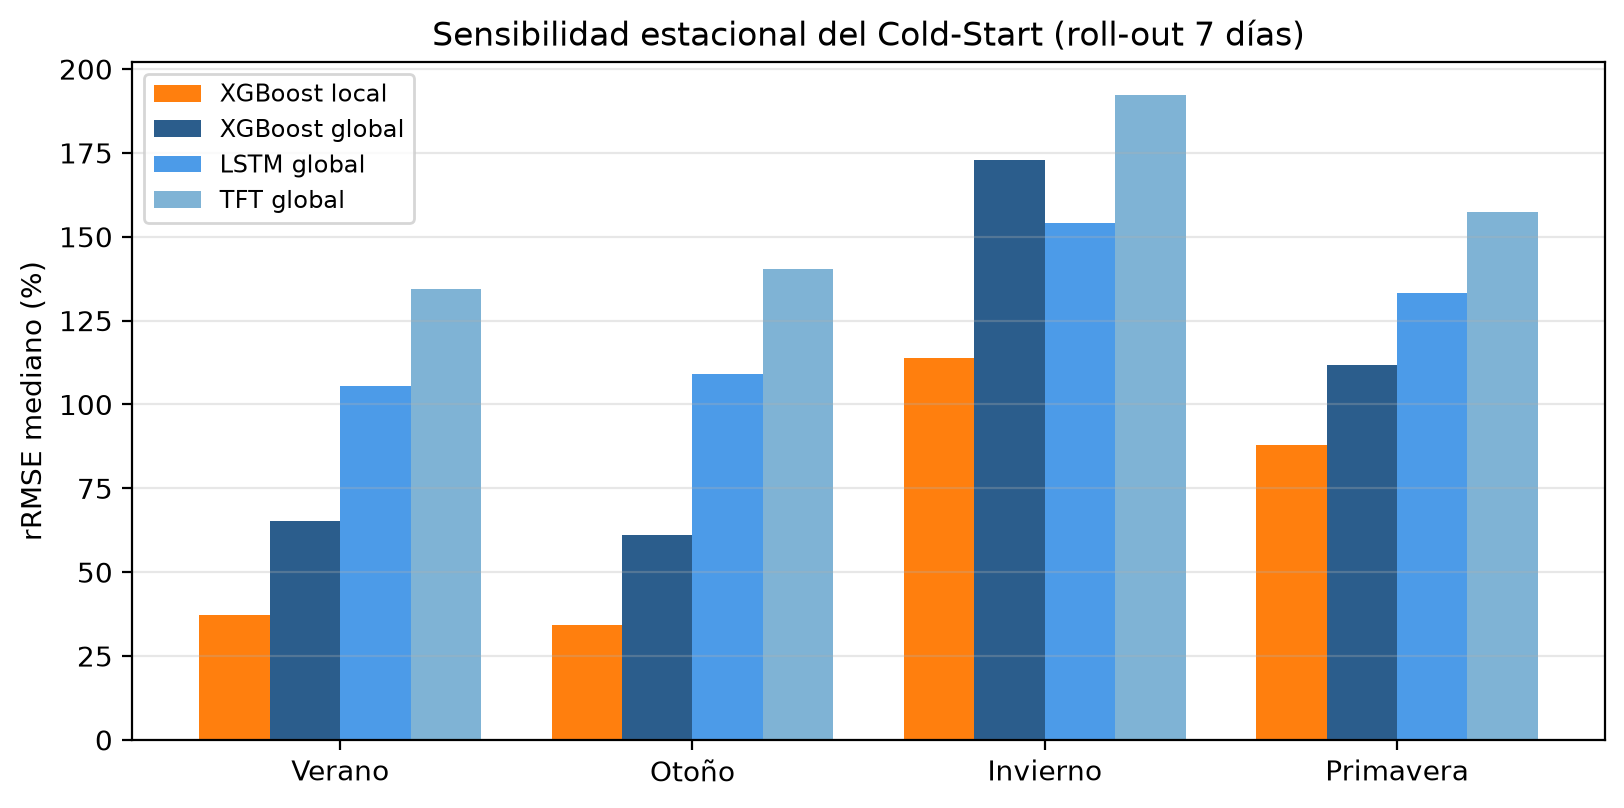
\includegraphics[width=\linewidth]{fig_estacional.png}
    \end{column}
    \begin{column}{0.5\textwidth}
      \textbf{rRMSE roll-out por estación}
      \vspace{0.3em}

      \begin{itemize}
        \item XGBoost global: \; 52\,\% (verano) $\rightarrow$ \rj{134\,\%} (invierno)
        \item XGBoost local: \; 40\,\% $\rightarrow$ \rj{115\,\%}
      \end{itemize}
      \vspace{0.5em}
      Mayor variabilidad nubosa y menor irradiación invernal debilitan la señal determinista del perfil solar.
      \vspace{0.5em}

      \textbf{Implicación operativa:} la incertidumbre de un parque nuevo depende fuertemente de la \textbf{estación de su puesta en marcha}.
    \end{column}
  \end{columns}
\end{frame}

\begin{frame}{Calidad probabilística: la calibración no se transfiere}
  \small
  \begin{center}
  \begin{tabular}{llcc}
    \toprule
    Config. & Tipo & Cobertura diurna & Pinball P95 (MWh) \\
    \midrule
    XGBoost  & \lo{Local}  & \textbf{0,86} & \textbf{0,035} \\
    XGBoost  & \gl{Global} & 0,97 (sobre-cubre) & 0,092 \\
    LSTM     & \gl{Global} & 0,53 & 0,159 \\
    Informer & \gl{Global} & 0,64 & 0,115 \\
    TFT      & \gl{Global} & 0,38 & 0,158 \\
    N-HiTS   & \gl{Global} & 0,37 & 0,372 \\
    \bottomrule
  \end{tabular}
  \end{center}
  \normalsize
  \begin{itemize}
    \item Nominal = 0,90. \textbf{Ningún paradigma calibra idealmente}, con desvíos opuestos.
    \item Redes globales \rj{subcalibradas} (bandas demasiado estrechas); XGBoost global \rj{sobre-cubre}.
    \item \lo{XGBoost local} es el más cercano al nominal y con menor pinball.
  \end{itemize}
\end{frame}

\begin{frame}{Contraste de la hipótesis --- con test estadístico}
  % OJO: dentro de un título de bloque NO usar \rj/\lo/\gl — el fondo ya es de color
  % y el texto quedaría invisible (rojo sobre rojo). Se usa negrita sobre el blanco heredado.
  \begin{alertblock}{La hipótesis se \textbf{RECHAZA}, y ahora con significancia}
    \lo{XGBoost local} gana a \gl{XGBoost global} en \textbf{77 de 94 plantas}
    ($p<10^{-7}$, Wilcoxon pareado con corrección de Holm).
  \end{alertblock}
  \begin{block}{A igualdad de arquitectura: ningún global gana significativamente}
    \begin{itemize}
      \item \lo{N-HiTS local} supera a \gl{N-HiTS global} en \textbf{88/94} ($p<10^{-10}$).
      \item El par \textbf{LSTM} es un \rj{empate estadístico}: 49/45 plantas, $p=1{,}00$.
            El matiz que sugerían las medianas \textbf{no sobrevive} al test pareado.
    \end{itemize}
  \end{block}
  \begin{exampleblock}{El valor real: disponibilidad inmediata}
    En el arranque en frío puro (historia local nula) el modelo global \textbf{no tiene competidor local posible}.
  \end{exampleblock}
\end{frame}

\begin{frame}{Ejemplo de roll-out Cold-Start a 7 días}
  \centering
  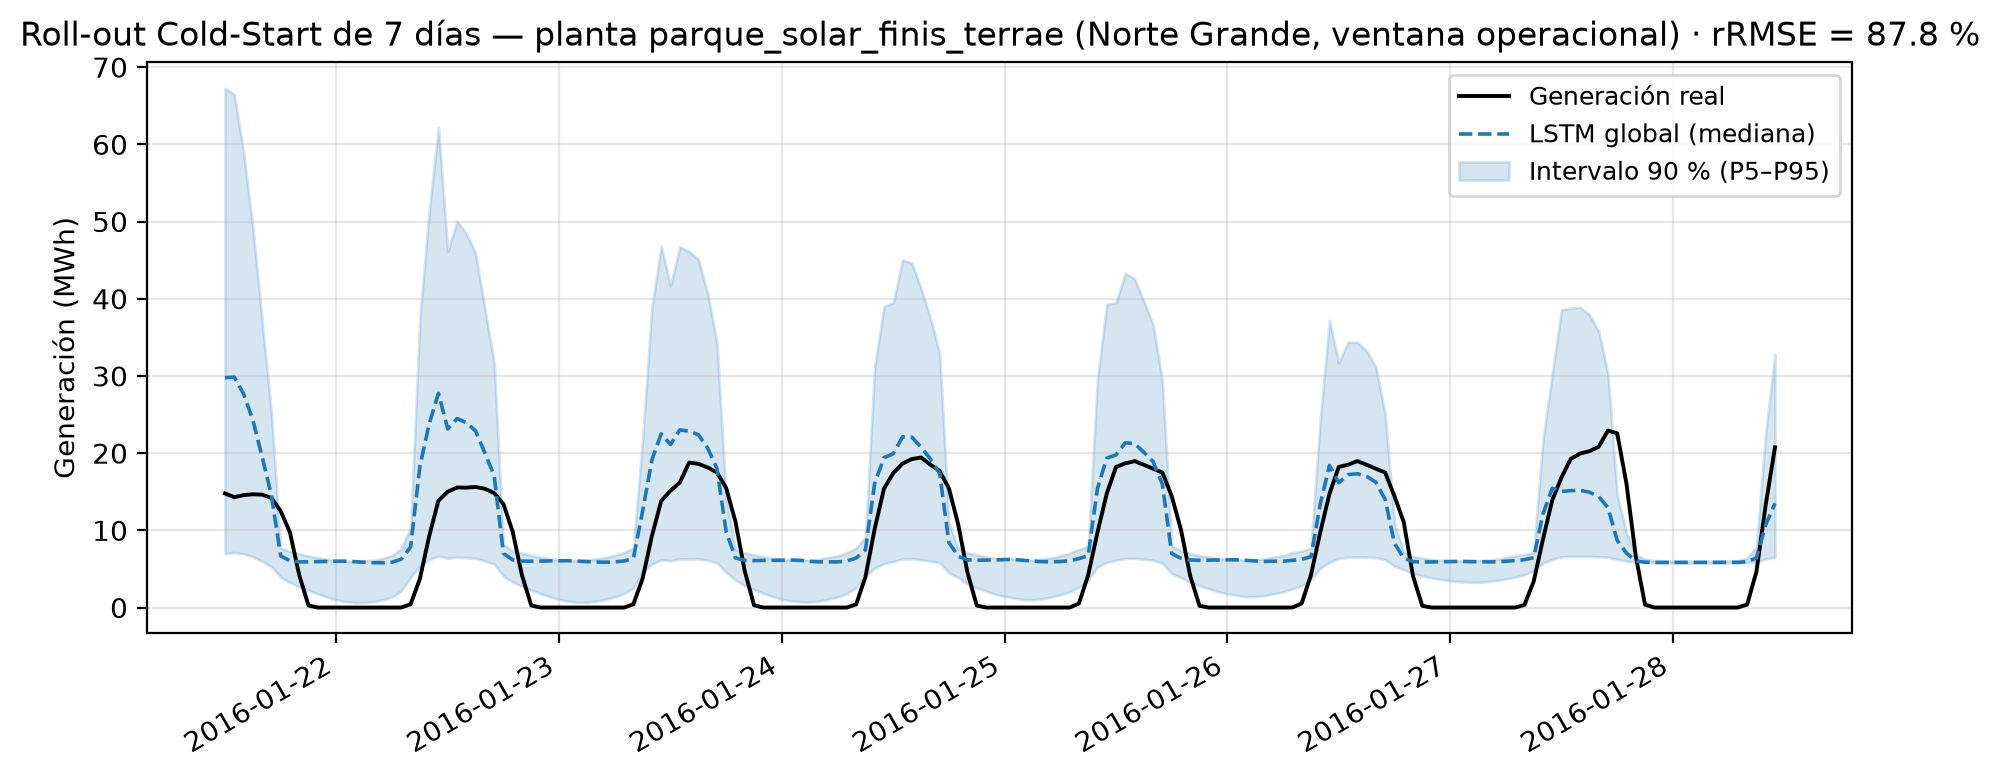
\includegraphics[width=0.9\textwidth]{fig_ejemplo_rollout.png}

  {\footnotesize El modelo global, \textbf{sin haber visto jamás la planta}, reproduce el ciclo diario y la magnitud de los picos usando solo el clima entrante y la geografía estática.}
\end{frame}

% ==================================================================
\section{Conclusiones}
% ==================================================================

\begin{frame}{Conclusiones}
  \begin{enumerate}
    \item \textbf{Resultado negativo riguroso:} bajo un protocolo estrictamente ciego, un XGBoost local maduro sigue siendo el estándar a batir. La hipótesis se rechaza.
    \item \textbf{El paradigma global conserva un régimen propio:} el arranque en frío puro, donde entrega pronósticos coherentes y accionables desde la hora cero.
    \item Cuatro hallazgos metodológicos transferibles:
    \begin{itemize}
      \item las rampas de puesta en marcha distorsionan las métricas (análisis Raw/Operacional);
      \item el invierno es sistemáticamente la estación más difícil;
      \item la calibración probabilística no se transfiere a las redes profundas;
      \item la integridad del \emph{target} (nunca imputar $y$) es esencial para la honestidad de las métricas.
    \end{itemize}
  \end{enumerate}
\end{frame}

\begin{frame}{Trabajo futuro}
  \begin{itemize}
    \item \textbf{Fine-tuning en dos etapas:} pre-entrenar global $\rightarrow$ ajustar con los primeros días reales; cierra la brecha con el local a medida que crece la historia.
    \item \textbf{Máscaras de intermitencia} en la atención: excluir la noche determinista y concentrar capacidad en la señal productiva.
    \item \textbf{Recalibración conformal} de los intervalos bajo transferencia.
    \item \textbf{Más datos y cómputo:} ampliar el corpus y el presupuesto de pasos (posible sub-entrenamiento de TFT/Informer en 6\,GB).
    \item \textbf{Máscara astronómica} para el forzamiento nocturno independiente de sensores.
  \end{itemize}
\end{frame}

\begin{frame}[plain]
  \centering
  \vfill
  {\usebeamercolor[fg]{structure}\Huge \textbf{Gracias}}\\[0.5em]
  {\Large ¿Preguntas?}\\[1.0em]
  
\includegraphics[width=0.13\linewidth]{figuras/logoUCM.png}\\[0.5em]
  \ifnum\confmode=1
    {\normalsize César David Aular Muñoz \quad·\quad Sergio Hernández}\\
    {\footnotesize cesaraular02@gmail.com \quad·\quad Universidad Católica del Maule}
  \else
    {\normalsize César David Aular Muñoz}\\
    {\footnotesize cesaraular02@gmail.com}
  \fi
  \vfill
\end{frame}

% ==================================================================
% BACKUP SLIDES — anticipando los ataques de la comisión
% ==================================================================
\appendix

\begin{frame}{Backup --- Tests estadísticos (Friedman + Wilcoxon-Holm)}
  \textbf{Diseño pareado y balanceado:} 94 plantas $\times$ 8 configuraciones sobre la
  misma grilla horaria canónica $\rightarrow$ aplica la comparación por rangos de
  Demšar (2006).
  \vspace{0.3em}
  \begin{itemize}
    \item \textbf{Friedman (omnibus):} $\chi^2 = 260{,}7$, $p < 10^{-50}$ — las
          configuraciones no son equivalentes.
    \item \textbf{Ranking medio} (1 = mejor): XGB local 1,80 · N-HiTS local 3,32 ·
          XGB global 3,34 · TFT 5,10 · Informer 5,15 · LSTM local 5,30 ·
          LSTM global 5,41 · N-HiTS global 6,59.
    \item \textbf{Mejor por planta:} XGB local en 60/94, XGB global en 15,
          N-HiTS local en 10.
  \end{itemize}
  \vspace{0.2em}
  \begin{alertblock}{Por qué la mediana marginal engañaba}
    rRMSE mediano sugería \gl{LSTM global} (118\,\%) mejor que \lo{LSTM local}
    (147\,\%). Pero la \textbf{mediana de las diferencias por planta} es $\approx 0$ y
    levemente a favor del local: la brecha la producían unas pocas plantas donde el
    local falla mucho, no una ventaja sistemática del global.
  \end{alertblock}
\end{frame}

\begin{frame}{Backup --- Causalidad temporal de los baselines locales}
  \begin{block}{Qué se hizo exactamente}
    Los baselines locales se entrenan con la historia \textbf{completa} de la planta
    \textbf{menos todas las ventanas de evaluación} (Raw, Operacional y las 4
    estacionales), con los \emph{lags} hacia esas ventanas enmascarados.
  \end{block}
  \begin{itemize}
    \item No hay fuga del \emph{target}: ningún rezago apunta dentro de una ventana.
    \item Pero el entrenamiento \textbf{sí incluye horas posteriores} a la ventana
          predicha $\rightarrow$ \rj{no es estrictamente causal}.
    \item Es una elección de diseño: representa el modelo maduro que el operador
          tendría \emph{tras acumular historia} — el rival más fuerte posible.
  \end{itemize}
  \begin{exampleblock}{Por qué esto refuerza la conclusión}
    El sesgo favorece al lado \lo{local}, que \textbf{gana}; y el espejo (LOPO oculta
    la planta pero \textbf{no el calendario}) favorece al lado \gl{global}, que
    \textbf{pierde igual}. Ambos sesgos empujan contra la conclusión reportada.
  \end{exampleblock}
\end{frame}

\begin{frame}{Backup --- Definición del RMSE}
  \begin{block}{Fórmula}
    \[
      \mathrm{RMSE} = \sqrt{\frac{1}{n}\sum_{i=1}^{n}\left(y_i - \hat{y}_i\right)^2}
    \]
  \end{block}
  \begin{itemize}
    \item Eleva al \textbf{cuadrado} cada error antes de promediar $\rightarrow$ penaliza las desviaciones grandes de forma \rj{cuadrática}, no lineal ni logarítmica.
    \item Ideal para el pronóstico FV: castiga con fuerza los errores en los \textbf{picos de inyección} de mediodía.
    \item Comparte unidades con la variable (MWh), a diferencia del MSE.
    \item \textbf{rRMSE} = RMSE normalizado por la generación media horaria de la ventana (ver backup siguiente).
  \end{itemize}
\end{frame}

\begin{frame}{Backup --- ¿Por qué el rRMSE supera el 100\,\%?}
  \[
    \mathrm{rRMSE} = \frac{\mathrm{RMSE}}{\overline{y}_{\text{ventana}}}\times 100
  \]
  \begin{itemize}
    \item El denominador $\overline{y}$ incluye las \textbf{horas nocturnas de generación nula}.
    \item Esto \textbf{deprime la media} y por tanto \textbf{infla} sistemáticamente el indicador.
    \item Valores $>100\,\%$ son \textbf{esperables} en pronóstico horario FV bajo esta normalización.
    \item Su valor no es la magnitud absoluta, sino la \rj{comparación relativa} entre arquitecturas sobre \textbf{ventanas idénticas}.
  \end{itemize}
  \vspace{0.3em}
  \centering\footnotesize
  Todas las configuraciones se comparan sobre la misma grilla horaria canónica $\rightarrow$ comparación estrictamente pareada.
\end{frame}

\begin{frame}{Backup --- Calibración de XGBoost (global vs.\ local)}
  \begin{columns}[T]
    \begin{column}{0.5\textwidth}
      \textbf{XGBoost global: 0,97 (sobre-cubre)}
      \begin{itemize}
        \item Regresión cuantílica sobre un contexto \textbf{heterogéneo} ($N-1$ plantas).
        \item Bandas \textbf{demasiado anchas}: casi nunca fallan, pero pierden utilidad operativa.
        \item Un defecto \textbf{simétrico} al de las redes, no una virtud.
      \end{itemize}
    \end{column}
    \begin{column}{0.5\textwidth}
      \textbf{XGBoost local: 0,86 (casi nominal)}
      \begin{itemize}
        \item Ajustado a la variabilidad \textbf{real} de la propia planta.
        \item Pinball P95 = \textbf{0,035} MWh vs.\ 0,092 del global.
        \item Intervalos más estrechos y \textbf{mejor centrados}.
      \end{itemize}
    \end{column}
  \end{columns}
  \vspace{0.5em}
  \begin{alertblock}{¿Por qué las redes profundas subcalibran?}
    Su escalador local se ajusta sobre el \textbf{contexto sintético}, cuya varianza (perfil solar idealizado) es menor que la real $\rightarrow$ bandas estrechas. Los baselines locales profundos, con contexto real, mejoran (LSTM local 0,79).
  \end{alertblock}
\end{frame}

\begin{frame}{Backup --- Detalles de cómputo}
  \begin{itemize}
    \item \textbf{Precisión fp32} completa: la mezcla fp16 introducía inestabilidad numérica en el entrenamiento.
    \item \textbf{GPU RTX 2060 (6\,GB):} la VRAM la gobierna \texttt{batch\_size}$\times$\texttt{windows\_batch\_size}, no el tamaño del corpus $\rightarrow$ no se trunca la historia.
    \item \textbf{Presupuesto por época corregido:} cada paso consume \texttt{batch}$\times$\texttt{windows\_batch} ventanas; la fórmula ingenua \texttt{filas/batch} sobreestimaba $\sim$250$\times$.
    \item \textbf{\emph{Early stopping}} sobre \texttt{val\_size}=168; tuning cacheado una vez por modelo y reusado entre folds (fuga a nivel de hiperparámetro: despreciable y documentada).
    \item Toda predicción se fuerza a $\hat{y}\geq 0$ y a cero de noche (consistencia física).
  \end{itemize}
\end{frame}

\begin{frame}{Backup --- Tabla completa (day1 y roll-out)}
  \scriptsize
  \begin{center}
  \begin{tabular}{llcccccc}
    \toprule
     & & \multicolumn{2}{c}{NRMSE (\% cap.)} & \multicolumn{2}{c}{rRMSE (\%)} & & \\
    \cmidrule(lr){3-4}\cmidrule(lr){5-6}
    Config. & Tipo & day1 & roll7d & day1 & roll7d & Cob. & Pinball \\
    \midrule
    XGBoost  & \lo{Local}  & \textbf{9,5} & \textbf{13,2} & 45,6 & 59,9 & 0,86 & 0,035 \\
    XGBoost  & \gl{Global} & 15,6 & 17,1 & 64,0 & 75,1 & 0,97 & 0,092 \\
    N-HiTS   & \lo{Local}  & 14,2 & 17,6 & 62,3 & 85,2 & 0,72 & 0,096 \\
    Informer & \gl{Global} & 21,0 & 22,8 & 96,6 & 106,5 & 0,64 & 0,115 \\
    TFT      & \gl{Global} & 22,0 & 23,6 & 105,1 & 112,7 & 0,38 & 0,158 \\
    LSTM     & \lo{Local}  & 16,3 & 23,9 & 102,6 & 128,8 & 0,72 & 0,235 \\
    LSTM     & \gl{Global} & 22,6 & 24,8 & 99,7 & 108,6 & 0,53 & 0,159 \\
    N-HiTS   & \gl{Global} & 28,6 & 30,7 & 129,8 & 148,2 & 0,37 & 0,372 \\
    \bottomrule
  \end{tabular}
  \end{center}
  \normalsize
  \centering Ventana \emph{cold-start}, mediana sobre las \textbf{94 plantas}
  (Operacional donde hay rampa $>$24\,h; Raw en el resto).
\end{frame}

\end{document}
"
% Solo cambian portada/autores/afiliacion/evento; el contenido es el mismo.
% ====================================================================
\providecommand{\confmode}{0}% 0 = defensa, 1 = conferencia
\usepackage[utf8]{inputenc}
\usepackage[T1]{fontenc}
\usepackage[spanish,es-noquoting]{babel}
% Evita el "Incompatible glue units" de babel-spanish al usar \% dentro de beamer
\makeatletter
\let\es@sppercent\relax
\makeatother
\usepackage{graphicx}
\usepackage{booktabs}
\usepackage{amsmath}
\usepackage{xcolor}

\graphicspath{{figuras/}}

% --- Metadatos (usados por la plantilla oficial en portada, pie y cabecera) ---
\ifnum\confmode=1
  % ----- Modo CONFERENCIA (paper IEEE) -----
  \title[Pronóstico FV \emph{Cold-Start} · LOPO]{Pronóstico fotovoltaico a corto plazo bajo escasez de datos mediante evaluación \emph{Leave-One-Plant-Out}}
  \subtitle{Un enfoque \emph{Cross-Site} multi-planta frente a modelos locales}
  \author[Aular \& Hernández]{César David Aular Muñoz \and Sergio Hernández}
  \institute[UCM]{Departamento de Computación e Industrias \\ Facultad de Ciencias de la Ingeniería \\ Universidad Católica del Maule}
  \date{Chilean Workshop on Pattern Recognition (CWPR) --- 2026}
\else
  % ----- Modo DEFENSA (examen de título) -----
  \title[Multi-sitio vs.\ local: pronóstico FV \emph{Cold-Start}]{Análisis comparativo de un enfoque multi-sitio frente a modelos locales para la proyección a corto plazo de generación fotovoltaica bajo escasez de datos}
  % \subtitle{Proyección a corto plazo de generación fotovoltaica bajo escasez de datos}
  \author[César Aular]{César David Aular Muñoz}
  \institute[Escuela ICI --- UCM]{Escuela Ingeniería Civil Informática \\ Universidad Católica del Maule}
  \date{Proyecto de Título --- Junio 2026}
\fi

% --- Plantilla oficial de presentación UCM (tema QUT: azul institucional #00407a) ---
\usepackage{QUT}

% --- Colores semánticos: global (azul) / local (verde) / alerta (rojo) ---
\definecolor{glob}{HTML}{1F77B4}
\definecolor{loc}{HTML}{2CA02C}
\definecolor{alertred}{HTML}{C0392B}
\newcommand{\gl}[1]{\textcolor{glob}{\textbf{#1}}}
\newcommand{\lo}[1]{\textcolor{loc}{\textbf{#1}}}
\newcommand{\rj}[1]{\textcolor{alertred}{\textbf{#1}}}

% --- Bloques redondeados con relleno (info=azul UCM / ejemplo=verde / alerta=rojo) ---
\setbeamertemplate{blocks}[rounded][shadow=true]
\setbeamercolor{block title}{bg=qut,fg=white}
\setbeamercolor{block body}{bg=qut!8,fg=black}
\setbeamercolor{block title example}{bg=loc,fg=white}
\setbeamercolor{block body example}{bg=loc!8,fg=black}
\setbeamercolor{block title alerted}{bg=alertred,fg=white}
\setbeamercolor{block body alerted}{bg=alertred!8,fg=black}

\begin{document}

\begin{frame}[plain]
  \titlepage
  \begin{center}
    
\includegraphics[width=0.16\linewidth]{figuras/logoUCM.png}
  \end{center}
\end{frame}

\begin{frame}{Agenda}
  \tableofcontents[hideallsubsections]
\end{frame}

% ==================================================================
\section{El problema}
% ==================================================================

\begin{frame}{El problema del \emph{Cold-Start} fotovoltaico}
  \begin{columns}[T]
    \begin{column}{0.56\textwidth}
      \begin{itemize}
        \item Una planta FV \textbf{recién conectada} no tiene historial de generación.
        \item Los modelos clásicos entrenan \textbf{uno por planta} con meses o años de datos locales.
        \item Aplicados a una planta nueva: \rj{no se pueden entrenar} o se degradan gravemente.
      \end{itemize}
      \vspace{0.4em}
      \begin{alertblock}{Consecuencia}
        Incertidumbre justo cuando más se necesita certeza $\rightarrow$ mayores costos de balance y riesgo financiero, en especial para los pequeños PMGD.
      \end{alertblock}
    \end{column}
    \begin{column}{0.44\textwidth}
      \centering
      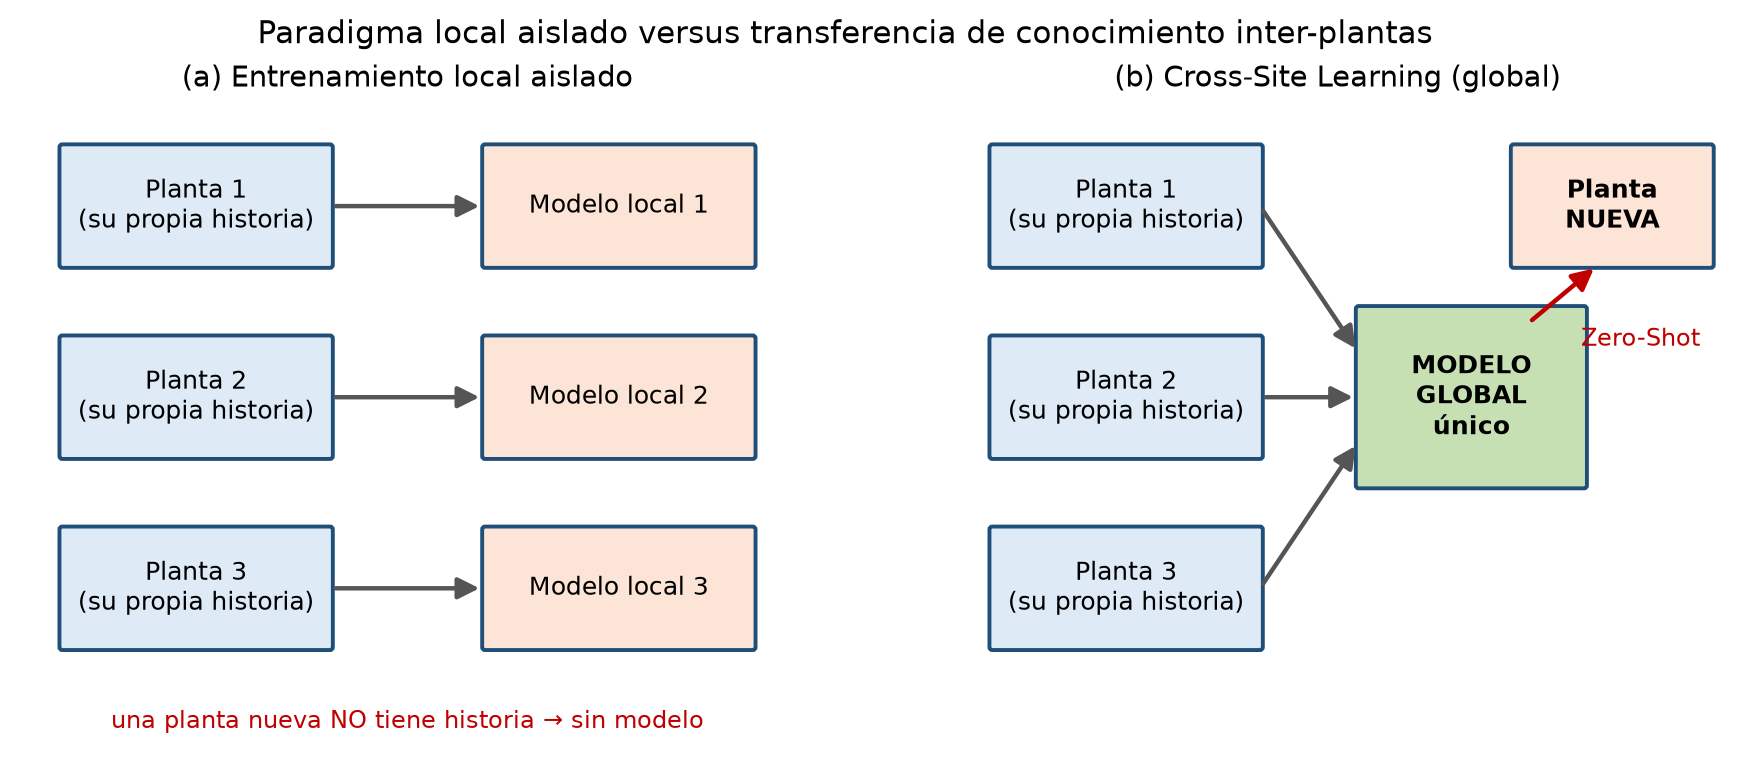
\includegraphics[width=\linewidth]{fig_cross_site.png}
      \vspace{0.3em}

      {\footnotesize El problema del arranque en frío, tomado de los sistemas de recomendación.}
    \end{column}
  \end{columns}
\end{frame}

\begin{frame}{La idea: aprendizaje \emph{Cross-Site}}
  \begin{columns}[T]
    \begin{column}{0.5\textwidth}
      Abandonar el supuesto \textbf{un-modelo-por-planta}.

      \vspace{0.6em}
      Un único modelo \gl{global} entrenado sobre \textbf{muchas plantas a la vez}:
      \begin{itemize}
        \item absorbe patrones compartidos clima~$\rightarrow$~potencia,
        \item los \textbf{transfiere} a una planta jamás vista,
        \item pronostica \textbf{desde la primera hora} de conexión.
      \end{itemize}
      \vspace{0.5em}
      \textbf{Pregunta central (adversarial):}\\
      \emph{¿realmente supera a una línea base local madura, o el premio de la transferencia se desvanece con una comparación justa?}
    \end{column}
    \begin{column}{0.5\textwidth}
      \centering
      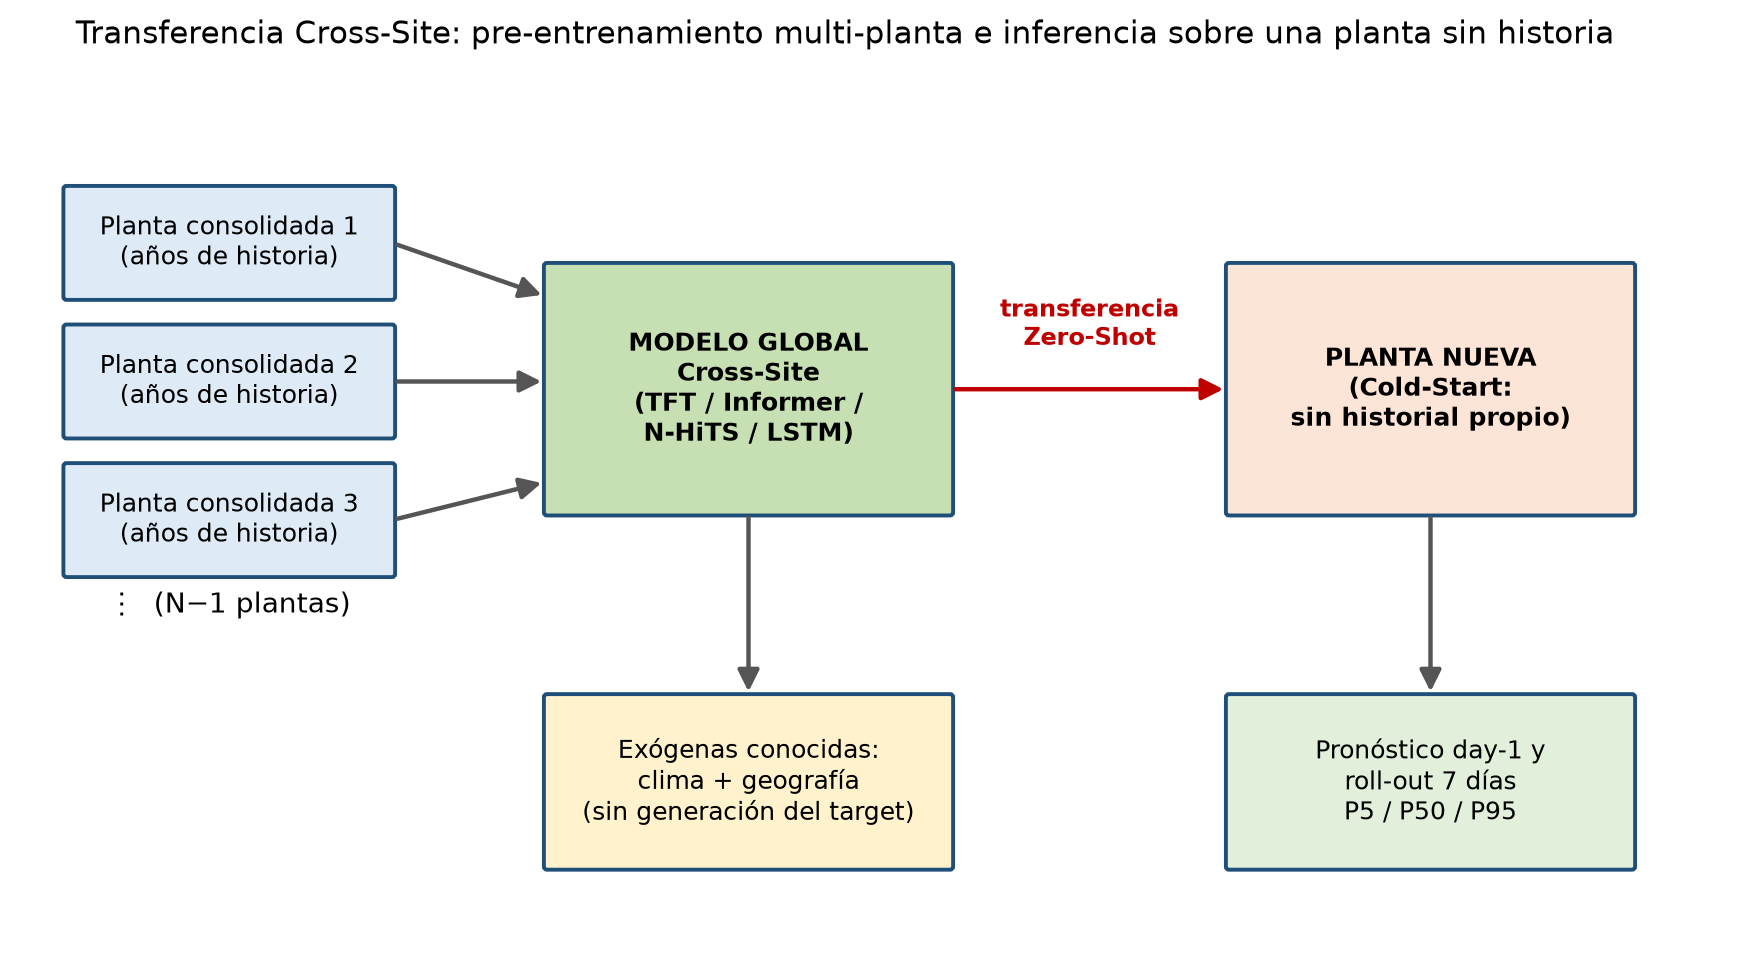
\includegraphics[width=\linewidth]{fig_solucion.png}
    \end{column}
  \end{columns}
\end{frame}

\begin{frame}{Hipótesis y objetivos}
  \begin{block}{Hipótesis}
    El modelo global multi-sitio es \emph{más preciso} que un modelo entrenado localmente con la historia propia del centro.
  \end{block}
  \begin{columns}[T]
    \begin{column}{0.5\textwidth}
      \textbf{Objetivos específicos}
      \begin{enumerate}
        \item Adaptar una arquitectura Transformer al entrenamiento multi-serie.
        \item Evaluarla frente a modelos locales bajo un protocolo \emph{Cold-Start} estricto.
        \item Integrar datos multimodales sin fuga de información.
      \end{enumerate}
    \end{column}
    \begin{column}{0.5\textwidth}
      \textbf{La brecha en la literatura}\\
      Rara vez se combinan a la vez:
      \begin{enumerate}
        \item evaluación \textbf{ciega} a la planta objetivo (sin \emph{fine-tuning}),
        \item contraste \textbf{justo} contra locales maduros,
        \item caracterización \textbf{probabilística}.
      \end{enumerate}
    \end{column}
  \end{columns}
\end{frame}

% ==================================================================
\section{Metodología}
% ==================================================================

\begin{frame}{Arquitectura del sistema}
  \centering
  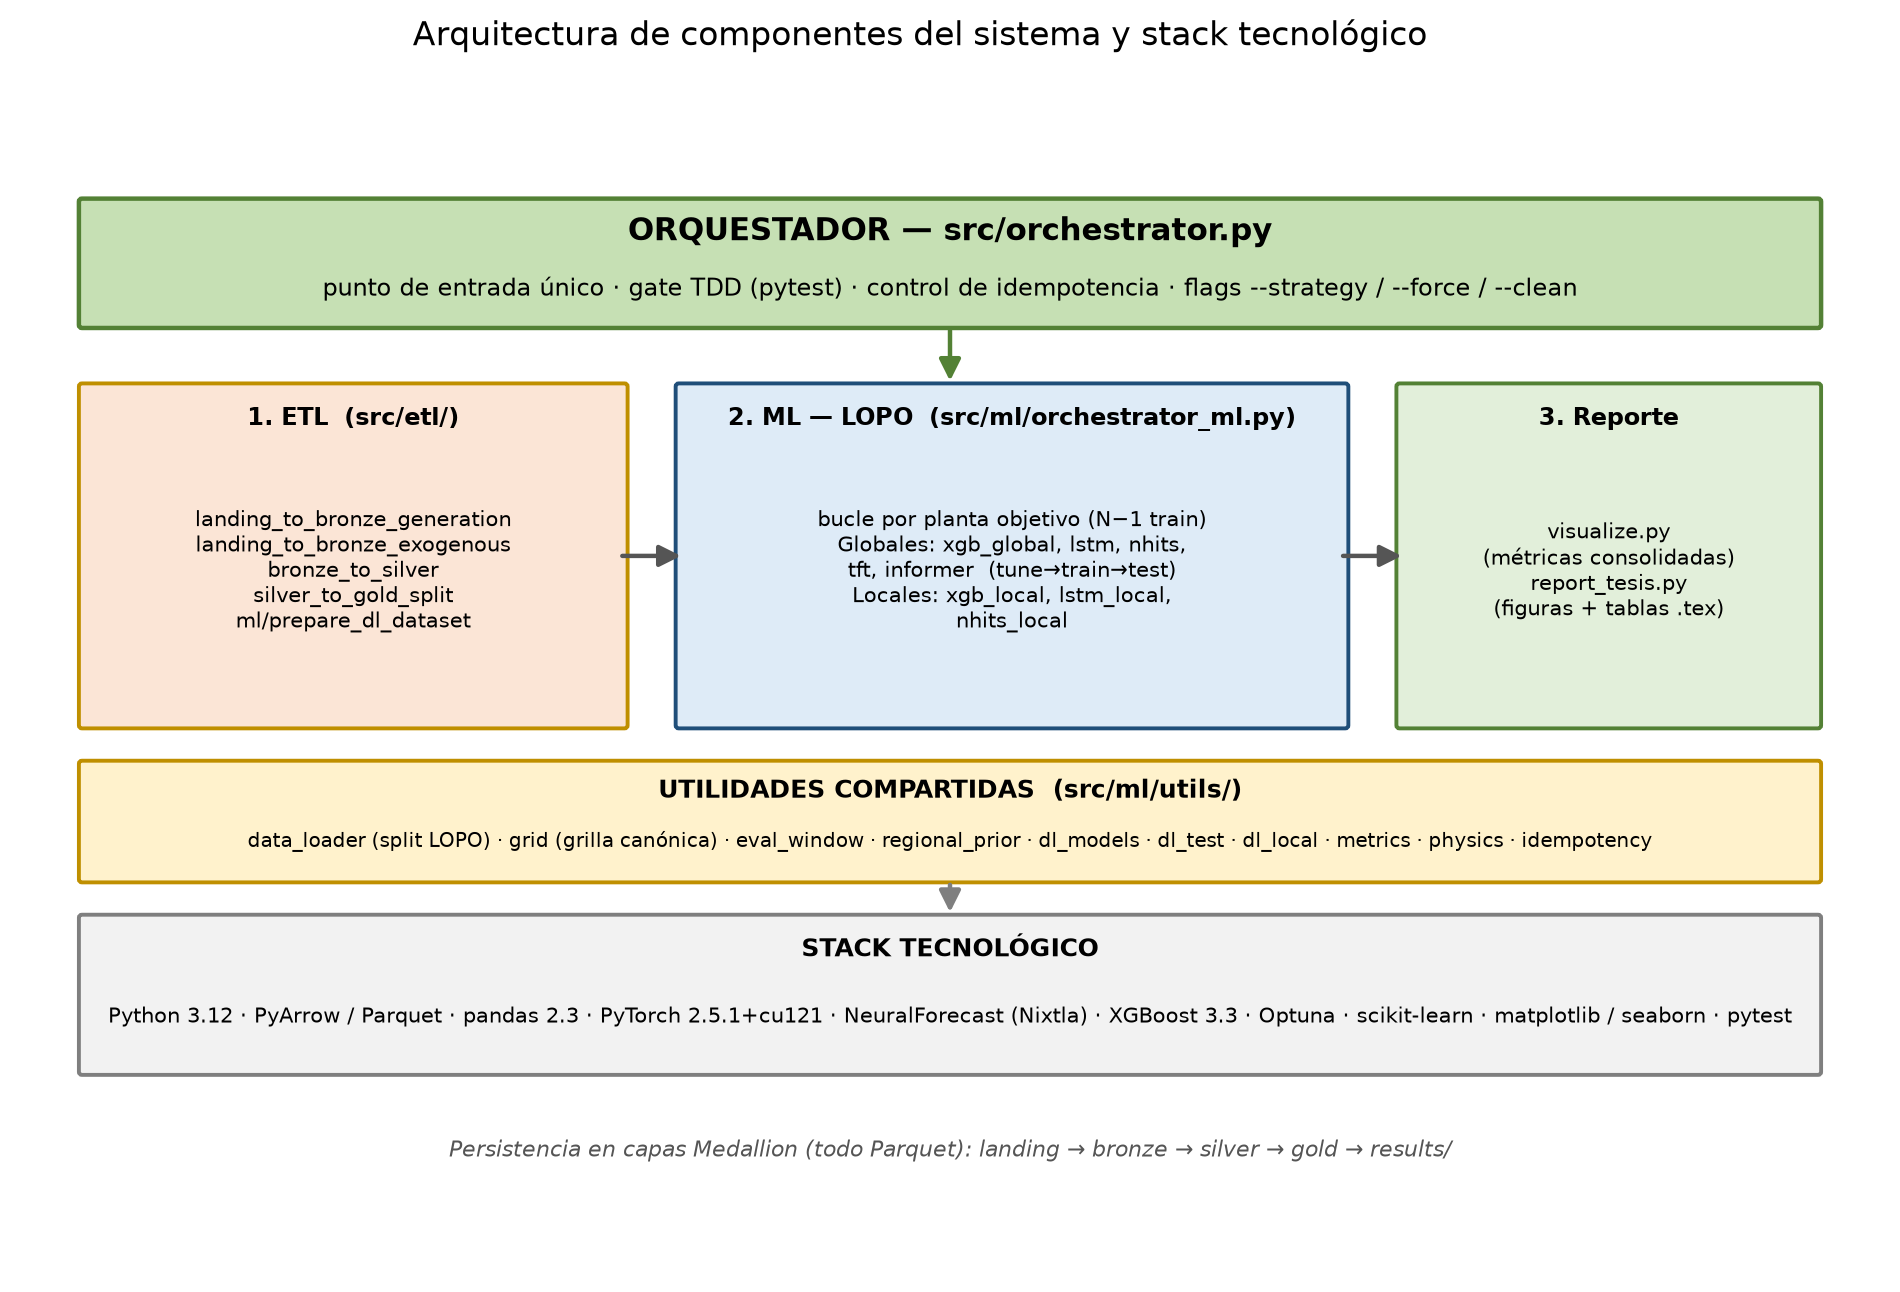
\includegraphics[height=0.78\textheight,keepaspectratio]{fig_arquitectura_componentes.png}
\end{frame}

\begin{frame}{Protocolo \emph{Leave-One-Plant-Out} (LOPO)}
  \begin{columns}[T]
    \begin{column}{0.52\textwidth}
      \begin{itemize}
        \item Para cada planta objetivo: los globales entrenan con las \textbf{$N-1$ restantes} (2014--2024 completo).
        \item La planta objetivo es \rj{invisible} durante el entrenamiento.
        \item Métricas: \textbf{mediana} sobre 94 plantas, solo observaciones reales.
      \end{itemize}
      \begin{exampleblock}{Integridad Zero-Shot (no negociable)}
        Ninguna variable puede ser función de la generación del objetivo. Verificado por pruebas automatizadas.
      \end{exampleblock}
    \end{column}
    \begin{column}{0.48\textwidth}
      \centering
      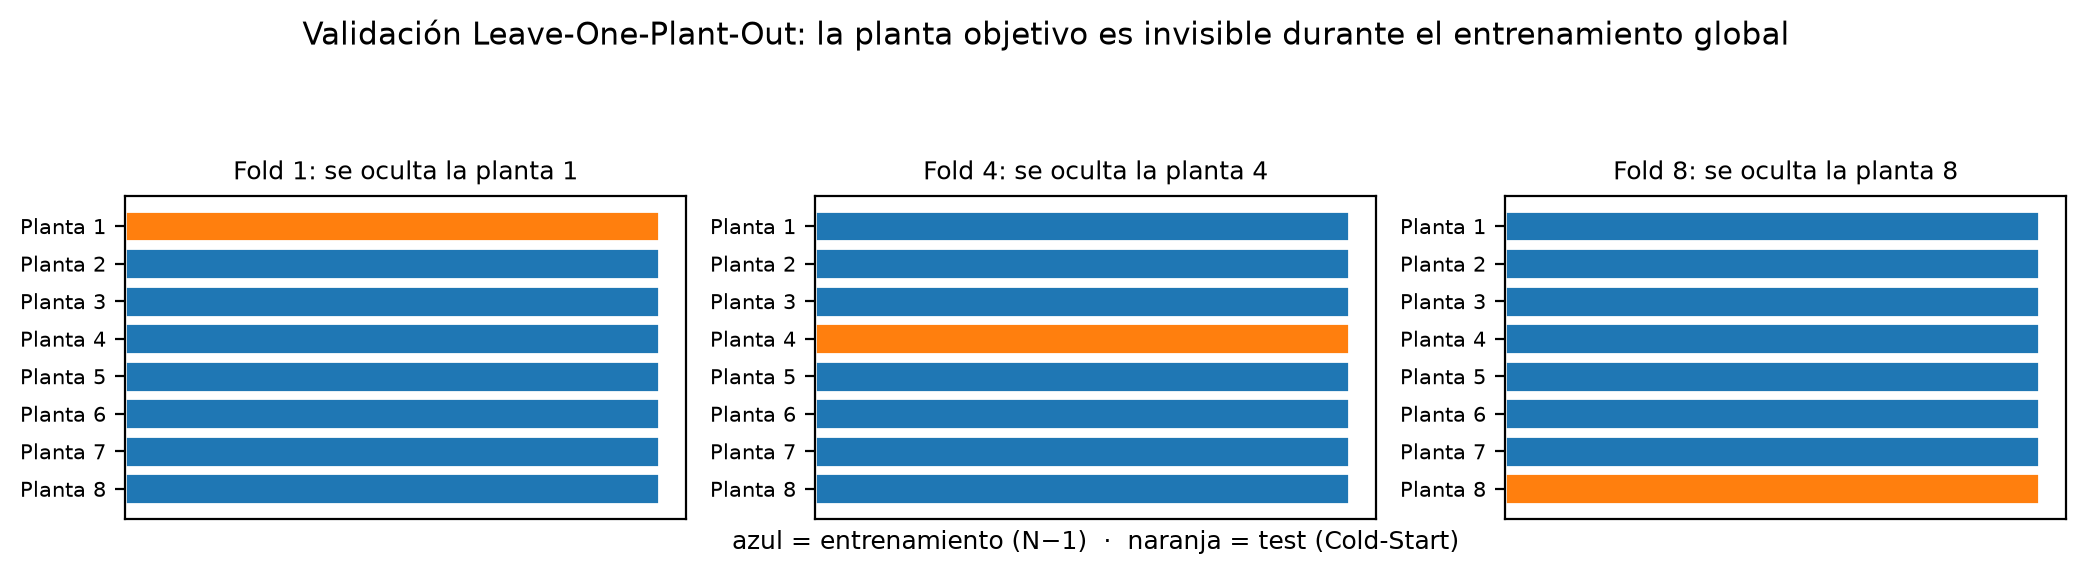
\includegraphics[width=\linewidth]{fig_lopo.png}
    \end{column}
  \end{columns}
\end{frame}

\begin{frame}{La lección de la fuga de datos}
  \begin{center}
    \Large Un \emph{prior} de eficiencia calculado \textbf{por-fila} desde el objetivo
  \end{center}
  \vspace{0.3em}
  \[
    PR = \frac{y}{\text{capacidad}} \quad\Longrightarrow\quad \mathrm{corr}(PR,\,y)=1.0
  \]
  \vspace{0.2em}
  \begin{columns}[T]
    \begin{column}{0.5\textwidth}
      \begin{alertblock}{rRMSE falso}
        $\approx 0.8\,\%$ \; (demasiado bueno para ser verdad)
      \end{alertblock}
    \end{column}
    \begin{column}{0.5\textwidth}
      \begin{exampleblock}{rRMSE honesto (tras corregir)}
        $\approx 56\,\%$
      \end{exampleblock}
    \end{column}
  \end{columns}
  \vspace{0.6em}
  \centering
  El \emph{prior} regional se agrega \textbf{solo sobre las plantas de entrenamiento} (por macrozona y estación).
\end{frame}

\begin{frame}{Semilla \emph{Cold-Start} sintética}
  Los modelos profundos necesitan una ventana de contexto que la planta nueva no tiene. Se siembra sintéticamente:
  \[
    \hat{y}_{\text{seed}}(t) = \text{capacidad}\cdot PR_{\text{regional}}\cdot s(t)
  \]
  \begin{itemize}
    \item $s(t)$: perfil solar determinista; $PR_{\text{regional}}$: solo plantas de entrenamiento.
    \item Solo el clima exógeno (conocido/pronosticable) y la geografía estática usan valores reales del objetivo.
    \item La generación de contexto es \rj{100\% sintética} $\rightarrow$ cero fuga.
  \end{itemize}
  \vspace{-0.4em}
  \centering
  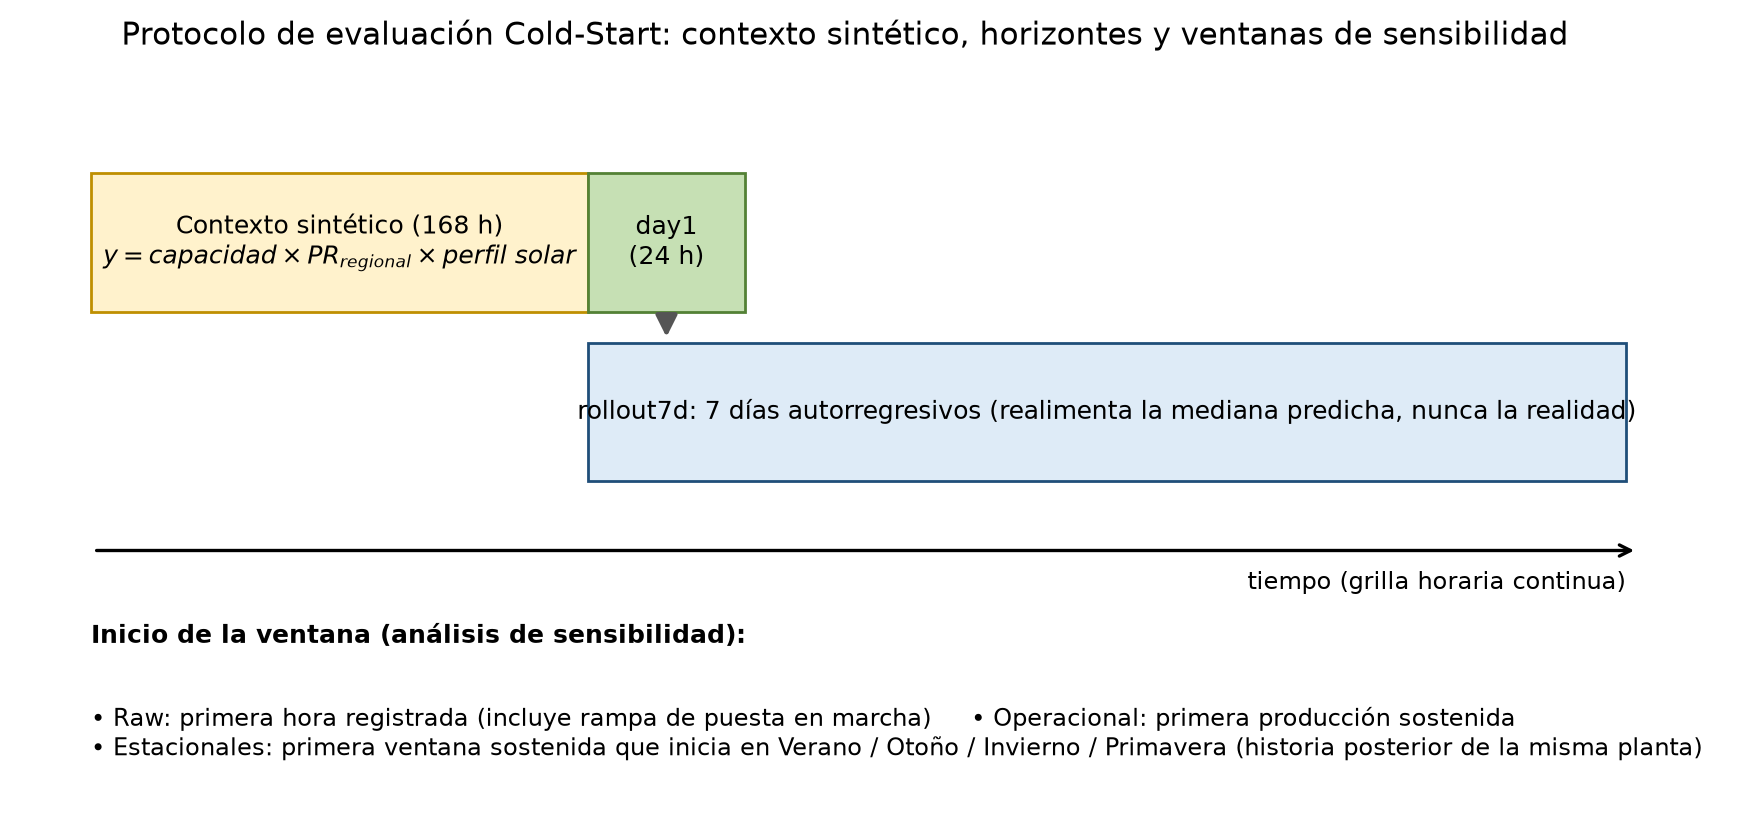
\includegraphics[width=0.54\textwidth]{fig_eval_protocolo.png}
\end{frame}

\begin{frame}{Ocho configuraciones y ventanas de evaluación}
  \begin{columns}[T]
    \begin{column}{0.48\textwidth}
      \textbf{5 globales \gl{(Cross-Site)}}
      \begin{itemize}
        \item TFT, Informer, N-HiTS, LSTM
        \item XGBoost global
      \end{itemize}
      \vspace{0.4em}
      \textbf{3 locales \lo{(estrictas)}}
      \begin{itemize}
        \item XGBoost, LSTM, N-HiTS
        \item entrenados solo con la historia propia
      \end{itemize}
      \vspace{0.5em}
      \textbf{Horizontes:} \emph{day1} (24\,h) y \emph{rollout7d} (7 días autorregresivos).
    \end{column}
    \begin{column}{0.52\textwidth}
      \centering
      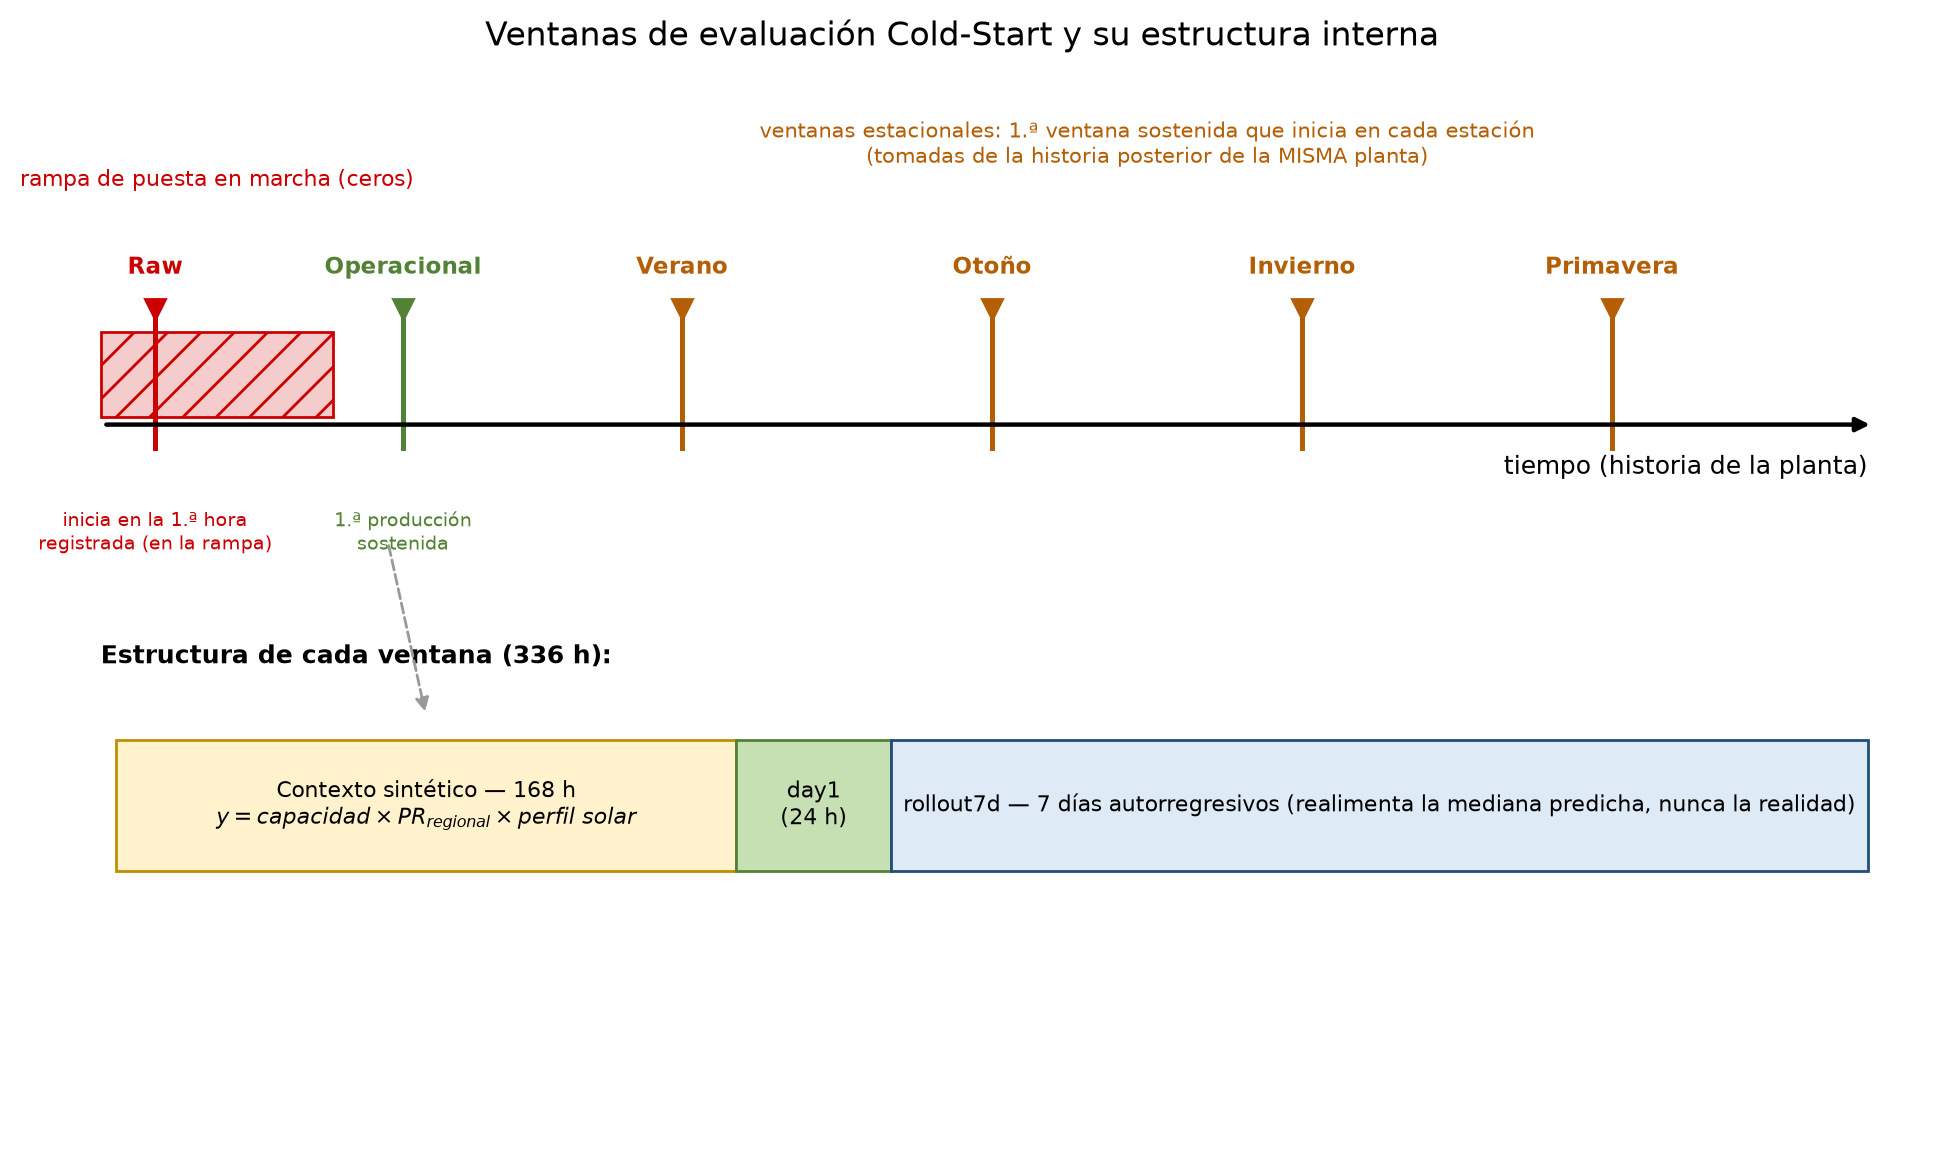
\includegraphics[width=\linewidth]{fig_ventanas_evaluacion.png}
      \vspace{0.2em}

      {\footnotesize \textbf{Raw} (incluye rampa) · \textbf{Operacional} (producción sostenida) · \textbf{Estacionales}.}
    \end{column}
  \end{columns}
\end{frame}

\begin{frame}{¿Dónde están las plantas? El corpus sobre el mapa}
  \begin{columns}[T]
    \begin{column}{0.42\textwidth}
      \centering
      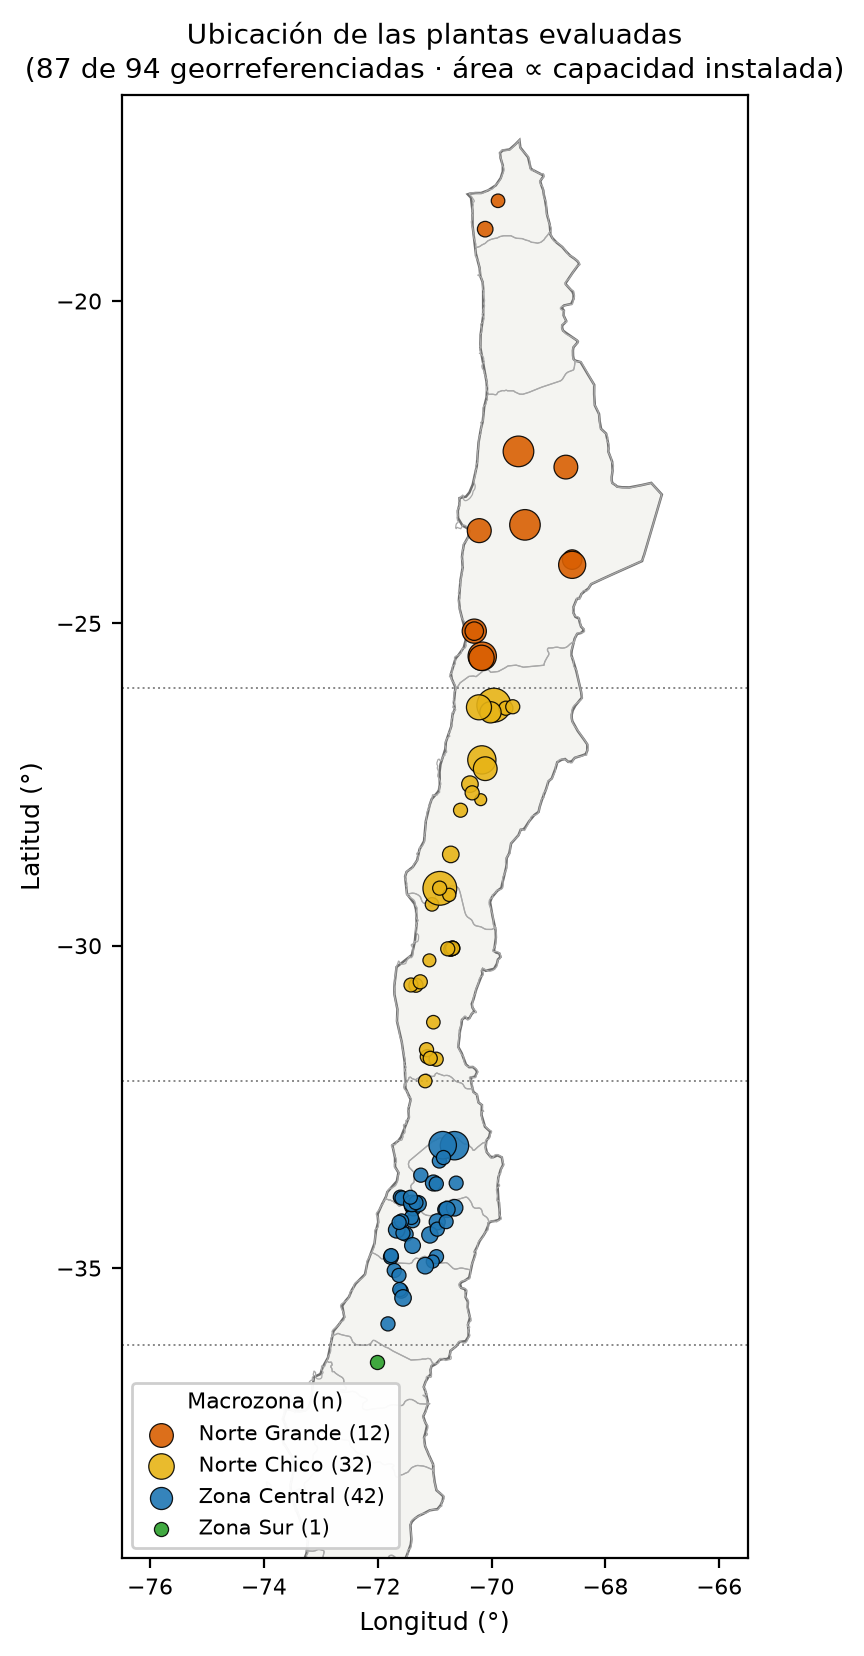
\includegraphics[height=0.78\textheight]{fig_mapa_plantas.png}
    \end{column}
    \begin{column}{0.58\textwidth}
      \vspace{1.2em}
      \begin{itemize}
        \item \textbf{94 plantas} del Sistema Eléctrico Nacional, a lo largo de todo el
              gradiente solar de Chile (Arica $\rightarrow$ zona sur).
        \item \gl{Norte Grande y Norte Chico}: pocas plantas pero \textbf{grandes}
              (utility scale, hasta 200\,MW) y de alta irradiancia.
        \item \lo{Zona Central}: muchas plantas \textbf{pequeñas} (PMGD, mediana
              $\approx$3\,MW) — el segmento que más sufre el arranque en frío.
      \end{itemize}
      \vspace{0.4em}
      \begin{exampleblock}{Por qué importa para la transferencia}
        La \textbf{macrozona} es la única señal espacial que ven los modelos, y es la
        clave sobre la que se agrega el \emph{prior} regional que siembra el contexto
        sintético.
      \end{exampleblock}
    \end{column}
  \end{columns}
\end{frame}

% ==================================================================
\section{Resultados}
% ==================================================================

\begin{frame}{Precisión puntual --- ventana \emph{cold-start}, 94 plantas (roll-out 7 días)}
  \begin{columns}[T]
    \begin{column}{0.46\textwidth}
      \small
      \begin{tabular}{llrr}
        \toprule
        Config. & Tipo & NRMSE & rRMSE \\
        \midrule
        XGBoost & \lo{Local}  & \textbf{13,2\,\%} & 60\,\% \\
        XGBoost & \gl{Global} & 17,1\,\% & 75\,\% \\
        N-HiTS  & \lo{Local}  & 17,6\,\% & 85\,\% \\
        Informer& \gl{Global} & 22,8\,\% & 107\,\% \\
        TFT     & \gl{Global} & 23,6\,\% & 113\,\% \\
        LSTM    & \lo{Local}  & 23,9\,\% & 129\,\% \\
        LSTM    & \gl{Global} & 24,8\,\% & 109\,\% \\
        N-HiTS  & \gl{Global} & 30,7\,\% & 148\,\% \\
        \bottomrule
      \end{tabular}

      \vspace{0.3em}
      {\scriptsize NRMSE = RMSE / capacidad instalada. \textbf{94 plantas}.}
    \end{column}
    \begin{column}{0.54\textwidth}
      \centering
      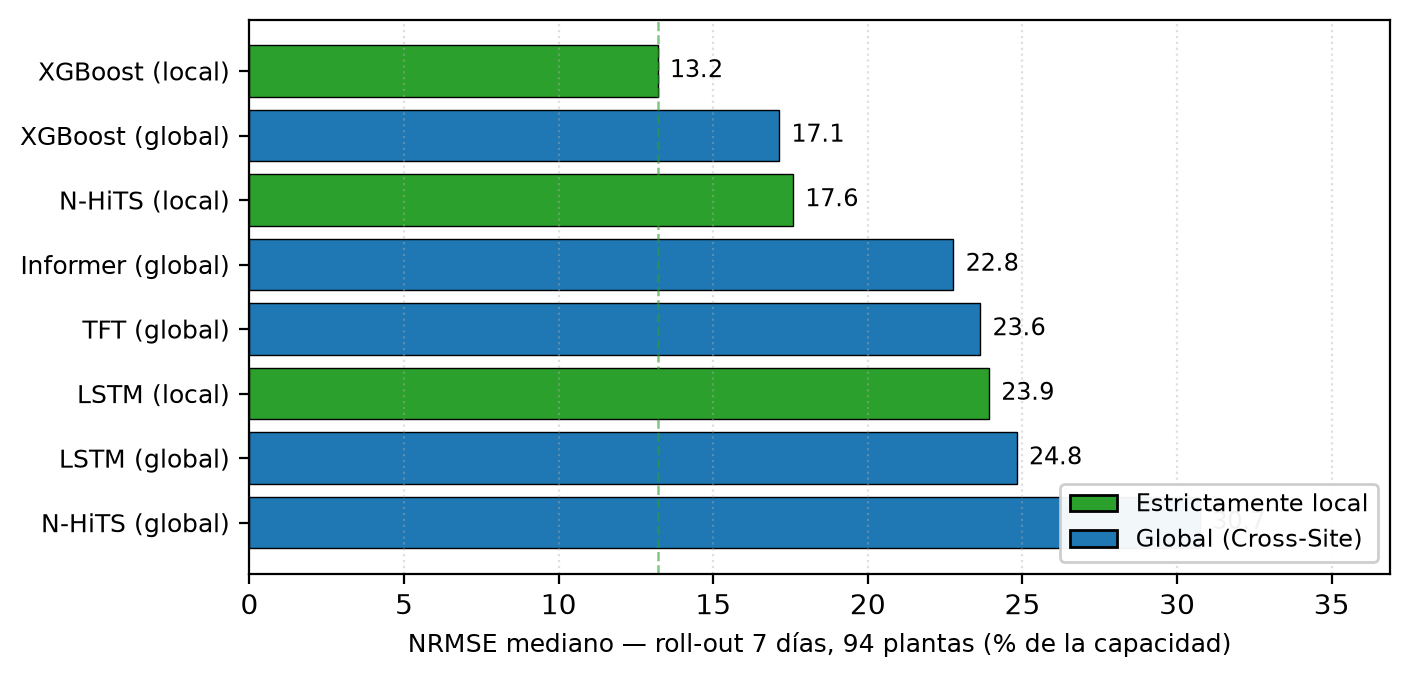
\includegraphics[width=\linewidth]{fig_resultados_nrmse_es.png}
    \end{column}
  \end{columns}
  \vspace{0.2em}
  {\footnotesize El \lo{XGBoost local} es el más preciso (13\,\% de la potencia nominal). Normalizar por \textbf{capacidad} hace los números interpretables —y cambia el orden del par LSTM respecto de rRMSE.}
\end{frame}

\begin{frame}{Sensibilidad estacional: el invierno es el gran desafío}
  \begin{columns}[T]
    \begin{column}{0.5\textwidth}
      \centering
      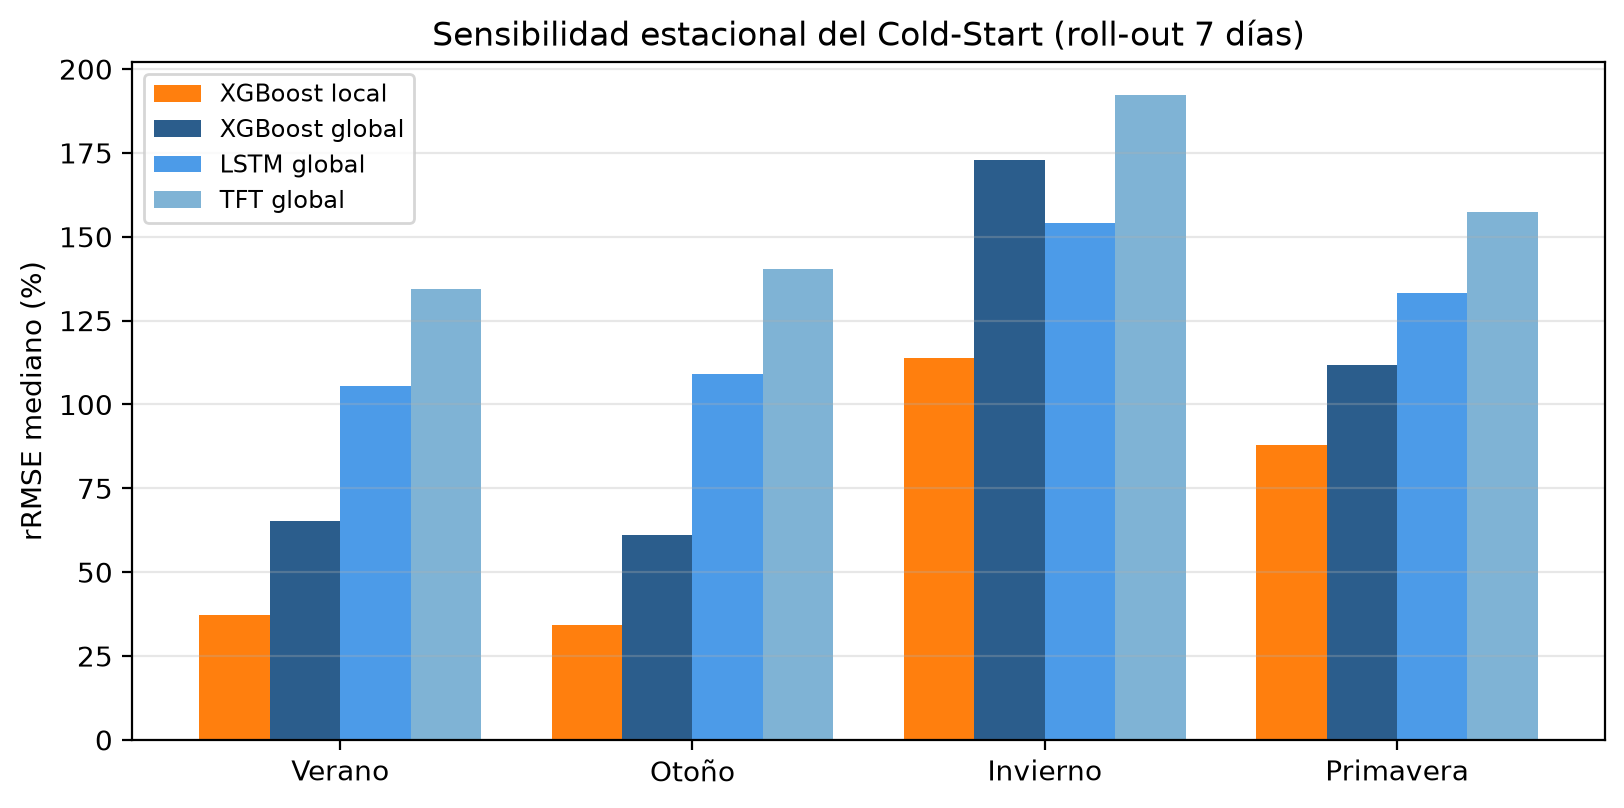
\includegraphics[width=\linewidth]{fig_estacional.png}
    \end{column}
    \begin{column}{0.5\textwidth}
      \textbf{rRMSE roll-out por estación}
      \vspace{0.3em}

      \begin{itemize}
        \item XGBoost global: \; 52\,\% (verano) $\rightarrow$ \rj{134\,\%} (invierno)
        \item XGBoost local: \; 40\,\% $\rightarrow$ \rj{115\,\%}
      \end{itemize}
      \vspace{0.5em}
      Mayor variabilidad nubosa y menor irradiación invernal debilitan la señal determinista del perfil solar.
      \vspace{0.5em}

      \textbf{Implicación operativa:} la incertidumbre de un parque nuevo depende fuertemente de la \textbf{estación de su puesta en marcha}.
    \end{column}
  \end{columns}
\end{frame}

\begin{frame}{Calidad probabilística: la calibración no se transfiere}
  \small
  \begin{center}
  \begin{tabular}{llcc}
    \toprule
    Config. & Tipo & Cobertura diurna & Pinball P95 (MWh) \\
    \midrule
    XGBoost  & \lo{Local}  & \textbf{0,86} & \textbf{0,035} \\
    XGBoost  & \gl{Global} & 0,97 (sobre-cubre) & 0,092 \\
    LSTM     & \gl{Global} & 0,53 & 0,159 \\
    Informer & \gl{Global} & 0,64 & 0,115 \\
    TFT      & \gl{Global} & 0,38 & 0,158 \\
    N-HiTS   & \gl{Global} & 0,37 & 0,372 \\
    \bottomrule
  \end{tabular}
  \end{center}
  \normalsize
  \begin{itemize}
    \item Nominal = 0,90. \textbf{Ningún paradigma calibra idealmente}, con desvíos opuestos.
    \item Redes globales \rj{subcalibradas} (bandas demasiado estrechas); XGBoost global \rj{sobre-cubre}.
    \item \lo{XGBoost local} es el más cercano al nominal y con menor pinball.
  \end{itemize}
\end{frame}

\begin{frame}{Contraste de la hipótesis --- con test estadístico}
  % OJO: dentro de un título de bloque NO usar \rj/\lo/\gl — el fondo ya es de color
  % y el texto quedaría invisible (rojo sobre rojo). Se usa negrita sobre el blanco heredado.
  \begin{alertblock}{La hipótesis se \textbf{RECHAZA}, y ahora con significancia}
    \lo{XGBoost local} gana a \gl{XGBoost global} en \textbf{77 de 94 plantas}
    ($p<10^{-7}$, Wilcoxon pareado con corrección de Holm).
  \end{alertblock}
  \begin{block}{A igualdad de arquitectura: ningún global gana significativamente}
    \begin{itemize}
      \item \lo{N-HiTS local} supera a \gl{N-HiTS global} en \textbf{88/94} ($p<10^{-10}$).
      \item El par \textbf{LSTM} es un \rj{empate estadístico}: 49/45 plantas, $p=1{,}00$.
            El matiz que sugerían las medianas \textbf{no sobrevive} al test pareado.
    \end{itemize}
  \end{block}
  \begin{exampleblock}{El valor real: disponibilidad inmediata}
    En el arranque en frío puro (historia local nula) el modelo global \textbf{no tiene competidor local posible}.
  \end{exampleblock}
\end{frame}

\begin{frame}{Ejemplo de roll-out Cold-Start a 7 días}
  \centering
  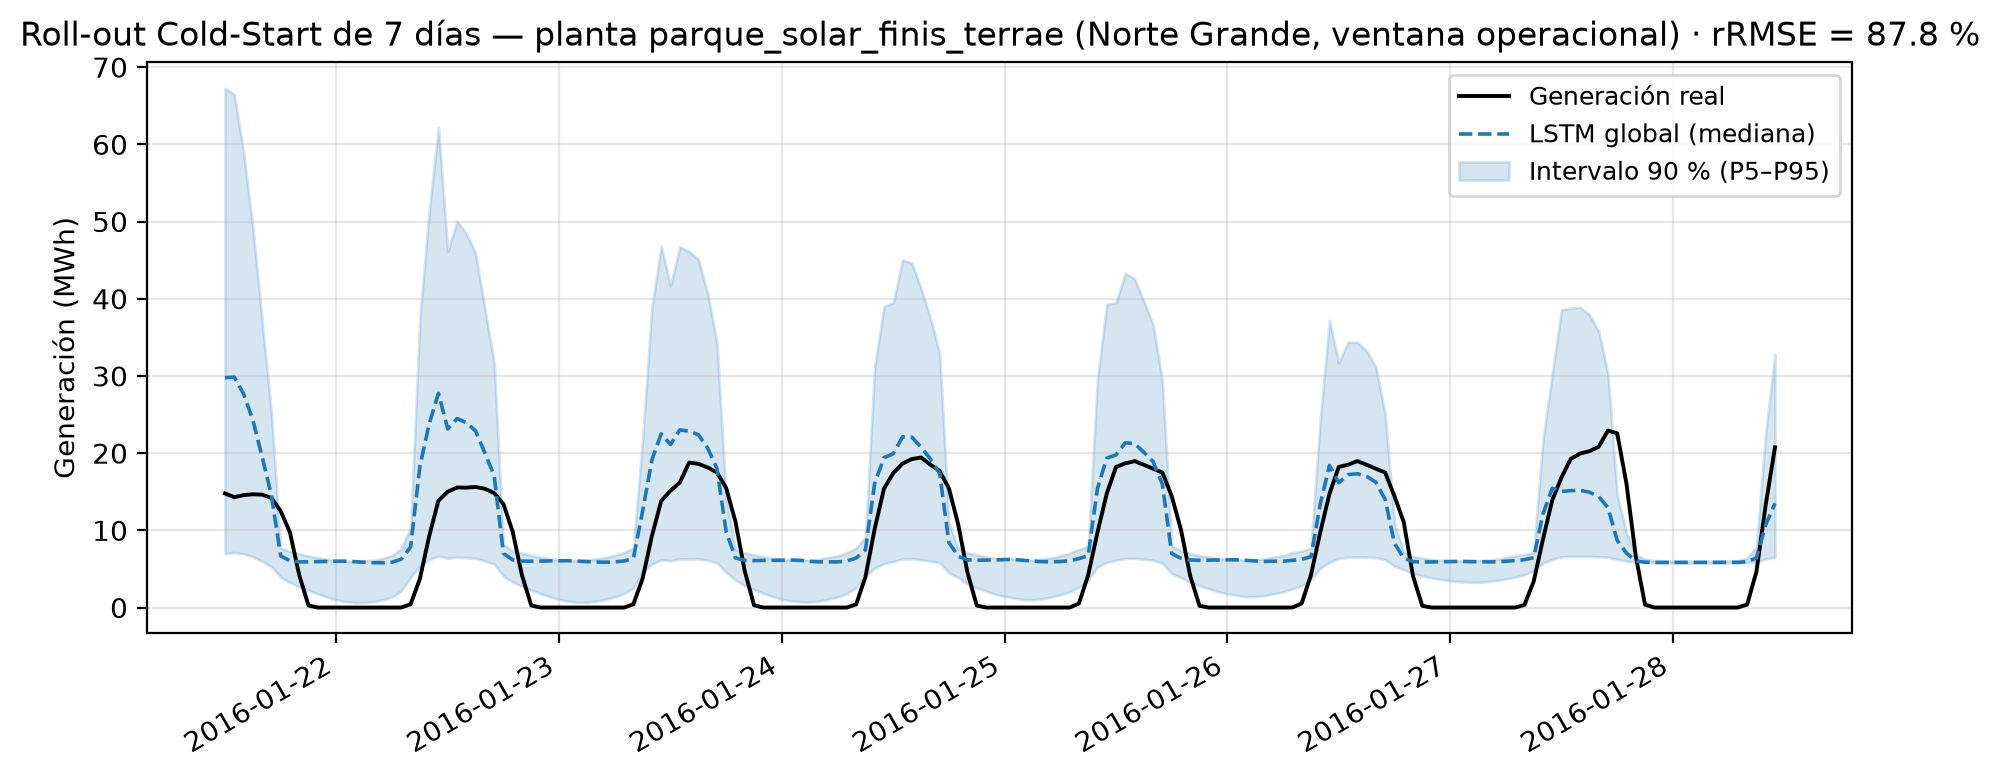
\includegraphics[width=0.9\textwidth]{fig_ejemplo_rollout.png}

  {\footnotesize El modelo global, \textbf{sin haber visto jamás la planta}, reproduce el ciclo diario y la magnitud de los picos usando solo el clima entrante y la geografía estática.}
\end{frame}

% ==================================================================
\section{Conclusiones}
% ==================================================================

\begin{frame}{Conclusiones}
  \begin{enumerate}
    \item \textbf{Resultado negativo riguroso:} bajo un protocolo estrictamente ciego, un XGBoost local maduro sigue siendo el estándar a batir. La hipótesis se rechaza.
    \item \textbf{El paradigma global conserva un régimen propio:} el arranque en frío puro, donde entrega pronósticos coherentes y accionables desde la hora cero.
    \item Cuatro hallazgos metodológicos transferibles:
    \begin{itemize}
      \item las rampas de puesta en marcha distorsionan las métricas (análisis Raw/Operacional);
      \item el invierno es sistemáticamente la estación más difícil;
      \item la calibración probabilística no se transfiere a las redes profundas;
      \item la integridad del \emph{target} (nunca imputar $y$) es esencial para la honestidad de las métricas.
    \end{itemize}
  \end{enumerate}
\end{frame}

\begin{frame}{Trabajo futuro}
  \begin{itemize}
    \item \textbf{Fine-tuning en dos etapas:} pre-entrenar global $\rightarrow$ ajustar con los primeros días reales; cierra la brecha con el local a medida que crece la historia.
    \item \textbf{Máscaras de intermitencia} en la atención: excluir la noche determinista y concentrar capacidad en la señal productiva.
    \item \textbf{Recalibración conformal} de los intervalos bajo transferencia.
    \item \textbf{Más datos y cómputo:} ampliar el corpus y el presupuesto de pasos (posible sub-entrenamiento de TFT/Informer en 6\,GB).
    \item \textbf{Máscara astronómica} para el forzamiento nocturno independiente de sensores.
  \end{itemize}
\end{frame}

\begin{frame}[plain]
  \centering
  \vfill
  {\usebeamercolor[fg]{structure}\Huge \textbf{Gracias}}\\[0.5em]
  {\Large ¿Preguntas?}\\[1.0em]
  
\includegraphics[width=0.13\linewidth]{figuras/logoUCM.png}\\[0.5em]
  \ifnum\confmode=1
    {\normalsize César David Aular Muñoz \quad·\quad Sergio Hernández}\\
    {\footnotesize cesaraular02@gmail.com \quad·\quad Universidad Católica del Maule}
  \else
    {\normalsize César David Aular Muñoz}\\
    {\footnotesize cesaraular02@gmail.com}
  \fi
  \vfill
\end{frame}

% ==================================================================
% BACKUP SLIDES — anticipando los ataques de la comisión
% ==================================================================
\appendix

\begin{frame}{Backup --- Tests estadísticos (Friedman + Wilcoxon-Holm)}
  \textbf{Diseño pareado y balanceado:} 94 plantas $\times$ 8 configuraciones sobre la
  misma grilla horaria canónica $\rightarrow$ aplica la comparación por rangos de
  Demšar (2006).
  \vspace{0.3em}
  \begin{itemize}
    \item \textbf{Friedman (omnibus):} $\chi^2 = 260{,}7$, $p < 10^{-50}$ — las
          configuraciones no son equivalentes.
    \item \textbf{Ranking medio} (1 = mejor): XGB local 1,80 · N-HiTS local 3,32 ·
          XGB global 3,34 · TFT 5,10 · Informer 5,15 · LSTM local 5,30 ·
          LSTM global 5,41 · N-HiTS global 6,59.
    \item \textbf{Mejor por planta:} XGB local en 60/94, XGB global en 15,
          N-HiTS local en 10.
  \end{itemize}
  \vspace{0.2em}
  \begin{alertblock}{Por qué la mediana marginal engañaba}
    rRMSE mediano sugería \gl{LSTM global} (118\,\%) mejor que \lo{LSTM local}
    (147\,\%). Pero la \textbf{mediana de las diferencias por planta} es $\approx 0$ y
    levemente a favor del local: la brecha la producían unas pocas plantas donde el
    local falla mucho, no una ventaja sistemática del global.
  \end{alertblock}
\end{frame}

\begin{frame}{Backup --- Causalidad temporal de los baselines locales}
  \begin{block}{Qué se hizo exactamente}
    Los baselines locales se entrenan con la historia \textbf{completa} de la planta
    \textbf{menos todas las ventanas de evaluación} (Raw, Operacional y las 4
    estacionales), con los \emph{lags} hacia esas ventanas enmascarados.
  \end{block}
  \begin{itemize}
    \item No hay fuga del \emph{target}: ningún rezago apunta dentro de una ventana.
    \item Pero el entrenamiento \textbf{sí incluye horas posteriores} a la ventana
          predicha $\rightarrow$ \rj{no es estrictamente causal}.
    \item Es una elección de diseño: representa el modelo maduro que el operador
          tendría \emph{tras acumular historia} — el rival más fuerte posible.
  \end{itemize}
  \begin{exampleblock}{Por qué esto refuerza la conclusión}
    El sesgo favorece al lado \lo{local}, que \textbf{gana}; y el espejo (LOPO oculta
    la planta pero \textbf{no el calendario}) favorece al lado \gl{global}, que
    \textbf{pierde igual}. Ambos sesgos empujan contra la conclusión reportada.
  \end{exampleblock}
\end{frame}

\begin{frame}{Backup --- Definición del RMSE}
  \begin{block}{Fórmula}
    \[
      \mathrm{RMSE} = \sqrt{\frac{1}{n}\sum_{i=1}^{n}\left(y_i - \hat{y}_i\right)^2}
    \]
  \end{block}
  \begin{itemize}
    \item Eleva al \textbf{cuadrado} cada error antes de promediar $\rightarrow$ penaliza las desviaciones grandes de forma \rj{cuadrática}, no lineal ni logarítmica.
    \item Ideal para el pronóstico FV: castiga con fuerza los errores en los \textbf{picos de inyección} de mediodía.
    \item Comparte unidades con la variable (MWh), a diferencia del MSE.
    \item \textbf{rRMSE} = RMSE normalizado por la generación media horaria de la ventana (ver backup siguiente).
  \end{itemize}
\end{frame}

\begin{frame}{Backup --- ¿Por qué el rRMSE supera el 100\,\%?}
  \[
    \mathrm{rRMSE} = \frac{\mathrm{RMSE}}{\overline{y}_{\text{ventana}}}\times 100
  \]
  \begin{itemize}
    \item El denominador $\overline{y}$ incluye las \textbf{horas nocturnas de generación nula}.
    \item Esto \textbf{deprime la media} y por tanto \textbf{infla} sistemáticamente el indicador.
    \item Valores $>100\,\%$ son \textbf{esperables} en pronóstico horario FV bajo esta normalización.
    \item Su valor no es la magnitud absoluta, sino la \rj{comparación relativa} entre arquitecturas sobre \textbf{ventanas idénticas}.
  \end{itemize}
  \vspace{0.3em}
  \centering\footnotesize
  Todas las configuraciones se comparan sobre la misma grilla horaria canónica $\rightarrow$ comparación estrictamente pareada.
\end{frame}

\begin{frame}{Backup --- Calibración de XGBoost (global vs.\ local)}
  \begin{columns}[T]
    \begin{column}{0.5\textwidth}
      \textbf{XGBoost global: 0,97 (sobre-cubre)}
      \begin{itemize}
        \item Regresión cuantílica sobre un contexto \textbf{heterogéneo} ($N-1$ plantas).
        \item Bandas \textbf{demasiado anchas}: casi nunca fallan, pero pierden utilidad operativa.
        \item Un defecto \textbf{simétrico} al de las redes, no una virtud.
      \end{itemize}
    \end{column}
    \begin{column}{0.5\textwidth}
      \textbf{XGBoost local: 0,86 (casi nominal)}
      \begin{itemize}
        \item Ajustado a la variabilidad \textbf{real} de la propia planta.
        \item Pinball P95 = \textbf{0,035} MWh vs.\ 0,092 del global.
        \item Intervalos más estrechos y \textbf{mejor centrados}.
      \end{itemize}
    \end{column}
  \end{columns}
  \vspace{0.5em}
  \begin{alertblock}{¿Por qué las redes profundas subcalibran?}
    Su escalador local se ajusta sobre el \textbf{contexto sintético}, cuya varianza (perfil solar idealizado) es menor que la real $\rightarrow$ bandas estrechas. Los baselines locales profundos, con contexto real, mejoran (LSTM local 0,79).
  \end{alertblock}
\end{frame}

\begin{frame}{Backup --- Detalles de cómputo}
  \begin{itemize}
    \item \textbf{Precisión fp32} completa: la mezcla fp16 introducía inestabilidad numérica en el entrenamiento.
    \item \textbf{GPU RTX 2060 (6\,GB):} la VRAM la gobierna \texttt{batch\_size}$\times$\texttt{windows\_batch\_size}, no el tamaño del corpus $\rightarrow$ no se trunca la historia.
    \item \textbf{Presupuesto por época corregido:} cada paso consume \texttt{batch}$\times$\texttt{windows\_batch} ventanas; la fórmula ingenua \texttt{filas/batch} sobreestimaba $\sim$250$\times$.
    \item \textbf{\emph{Early stopping}} sobre \texttt{val\_size}=168; tuning cacheado una vez por modelo y reusado entre folds (fuga a nivel de hiperparámetro: despreciable y documentada).
    \item Toda predicción se fuerza a $\hat{y}\geq 0$ y a cero de noche (consistencia física).
  \end{itemize}
\end{frame}

\begin{frame}{Backup --- Tabla completa (day1 y roll-out)}
  \scriptsize
  \begin{center}
  \begin{tabular}{llcccccc}
    \toprule
     & & \multicolumn{2}{c}{NRMSE (\% cap.)} & \multicolumn{2}{c}{rRMSE (\%)} & & \\
    \cmidrule(lr){3-4}\cmidrule(lr){5-6}
    Config. & Tipo & day1 & roll7d & day1 & roll7d & Cob. & Pinball \\
    \midrule
    XGBoost  & \lo{Local}  & \textbf{9,5} & \textbf{13,2} & 45,6 & 59,9 & 0,86 & 0,035 \\
    XGBoost  & \gl{Global} & 15,6 & 17,1 & 64,0 & 75,1 & 0,97 & 0,092 \\
    N-HiTS   & \lo{Local}  & 14,2 & 17,6 & 62,3 & 85,2 & 0,72 & 0,096 \\
    Informer & \gl{Global} & 21,0 & 22,8 & 96,6 & 106,5 & 0,64 & 0,115 \\
    TFT      & \gl{Global} & 22,0 & 23,6 & 105,1 & 112,7 & 0,38 & 0,158 \\
    LSTM     & \lo{Local}  & 16,3 & 23,9 & 102,6 & 128,8 & 0,72 & 0,235 \\
    LSTM     & \gl{Global} & 22,6 & 24,8 & 99,7 & 108,6 & 0,53 & 0,159 \\
    N-HiTS   & \gl{Global} & 28,6 & 30,7 & 129,8 & 148,2 & 0,37 & 0,372 \\
    \bottomrule
  \end{tabular}
  \end{center}
  \normalsize
  \centering Ventana \emph{cold-start}, mediana sobre las \textbf{94 plantas}
  (Operacional donde hay rampa $>$24\,h; Raw en el resto).
\end{frame}

\end{document}
"
% Solo cambian portada/autores/afiliacion/evento; el contenido es el mismo.
% ====================================================================
\providecommand{\confmode}{0}% 0 = defensa, 1 = conferencia
\usepackage[utf8]{inputenc}
\usepackage[T1]{fontenc}
\usepackage[spanish,es-noquoting]{babel}
% Evita el "Incompatible glue units" de babel-spanish al usar \% dentro de beamer
\makeatletter
\let\es@sppercent\relax
\makeatother
\usepackage{graphicx}
\usepackage{booktabs}
\usepackage{amsmath}
\usepackage{xcolor}

\graphicspath{{figuras/}}

% --- Metadatos (usados por la plantilla oficial en portada, pie y cabecera) ---
\ifnum\confmode=1
  % ----- Modo CONFERENCIA (paper IEEE) -----
  \title[Pronóstico FV \emph{Cold-Start} · LOPO]{Pronóstico fotovoltaico a corto plazo bajo escasez de datos mediante evaluación \emph{Leave-One-Plant-Out}}
  \subtitle{Un enfoque \emph{Cross-Site} multi-planta frente a modelos locales}
  \author[Aular \& Hernández]{César David Aular Muñoz \and Sergio Hernández}
  \institute[UCM]{Departamento de Computación e Industrias \\ Facultad de Ciencias de la Ingeniería \\ Universidad Católica del Maule}
  \date{Chilean Workshop on Pattern Recognition (CWPR) --- 2026}
\else
  % ----- Modo DEFENSA (examen de título) -----
  \title[Multi-sitio vs.\ local: pronóstico FV \emph{Cold-Start}]{Análisis comparativo de un enfoque multi-sitio frente a modelos locales para la proyección a corto plazo de generación fotovoltaica bajo escasez de datos}
  % \subtitle{Proyección a corto plazo de generación fotovoltaica bajo escasez de datos}
  \author[César Aular]{César David Aular Muñoz}
  \institute[Escuela ICI --- UCM]{Escuela Ingeniería Civil Informática \\ Universidad Católica del Maule}
  \date{Proyecto de Título --- Junio 2026}
\fi

% --- Plantilla oficial de presentación UCM (tema QUT: azul institucional #00407a) ---
\usepackage{QUT}

% --- Colores semánticos: global (azul) / local (verde) / alerta (rojo) ---
\definecolor{glob}{HTML}{1F77B4}
\definecolor{loc}{HTML}{2CA02C}
\definecolor{alertred}{HTML}{C0392B}
\newcommand{\gl}[1]{\textcolor{glob}{\textbf{#1}}}
\newcommand{\lo}[1]{\textcolor{loc}{\textbf{#1}}}
\newcommand{\rj}[1]{\textcolor{alertred}{\textbf{#1}}}

% --- Bloques redondeados con relleno (info=azul UCM / ejemplo=verde / alerta=rojo) ---
\setbeamertemplate{blocks}[rounded][shadow=true]
\setbeamercolor{block title}{bg=qut,fg=white}
\setbeamercolor{block body}{bg=qut!8,fg=black}
\setbeamercolor{block title example}{bg=loc,fg=white}
\setbeamercolor{block body example}{bg=loc!8,fg=black}
\setbeamercolor{block title alerted}{bg=alertred,fg=white}
\setbeamercolor{block body alerted}{bg=alertred!8,fg=black}

\begin{document}

\begin{frame}[plain]
  \titlepage
  \begin{center}
    
\includegraphics[width=0.16\linewidth]{figuras/logoUCM.png}
  \end{center}
\end{frame}

\begin{frame}{Agenda}
  \tableofcontents[hideallsubsections]
\end{frame}

% ==================================================================
\section{El problema}
% ==================================================================

\begin{frame}{El problema del \emph{Cold-Start} fotovoltaico}
  \begin{columns}[T]
    \begin{column}{0.56\textwidth}
      \begin{itemize}
        \item Una planta FV \textbf{recién conectada} no tiene historial de generación.
        \item Los modelos clásicos entrenan \textbf{uno por planta} con meses o años de datos locales.
        \item Aplicados a una planta nueva: \rj{no se pueden entrenar} o se degradan gravemente.
      \end{itemize}
      \vspace{0.4em}
      \begin{alertblock}{Consecuencia}
        Incertidumbre justo cuando más se necesita certeza $\rightarrow$ mayores costos de balance y riesgo financiero, en especial para los pequeños PMGD.
      \end{alertblock}
    \end{column}
    \begin{column}{0.44\textwidth}
      \centering
      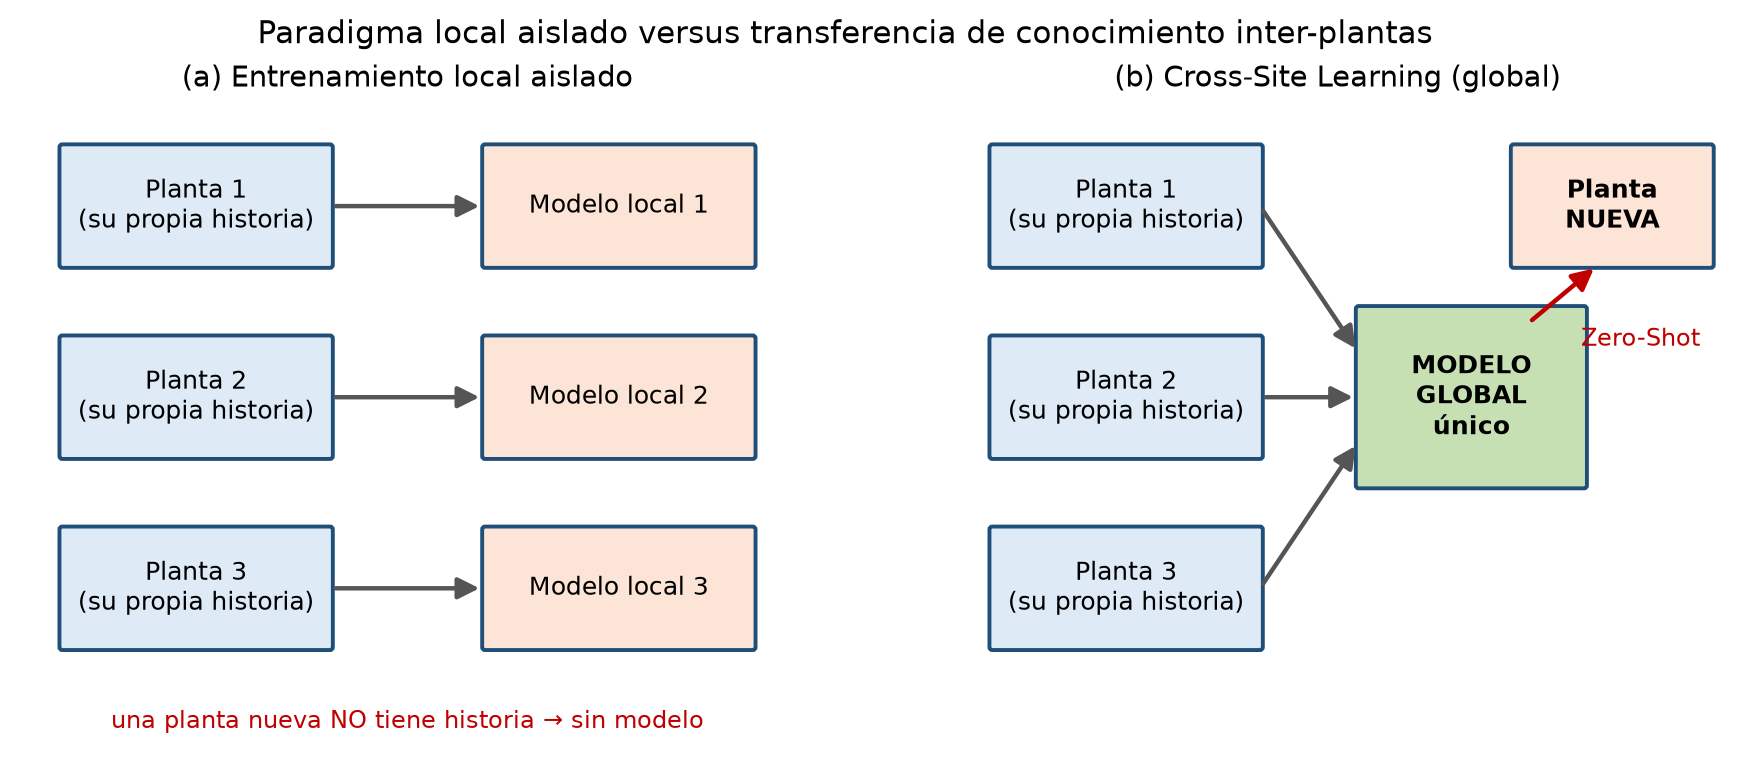
\includegraphics[width=\linewidth]{fig_cross_site.png}
      \vspace{0.3em}

      {\footnotesize El problema del arranque en frío, tomado de los sistemas de recomendación.}
    \end{column}
  \end{columns}
\end{frame}

\begin{frame}{La idea: aprendizaje \emph{Cross-Site}}
  \begin{columns}[T]
    \begin{column}{0.5\textwidth}
      Abandonar el supuesto \textbf{un-modelo-por-planta}.

      \vspace{0.6em}
      Un único modelo \gl{global} entrenado sobre \textbf{muchas plantas a la vez}:
      \begin{itemize}
        \item absorbe patrones compartidos clima~$\rightarrow$~potencia,
        \item los \textbf{transfiere} a una planta jamás vista,
        \item pronostica \textbf{desde la primera hora} de conexión.
      \end{itemize}
      \vspace{0.5em}
      \textbf{Pregunta central (adversarial):}\\
      \emph{¿realmente supera a una línea base local madura, o el premio de la transferencia se desvanece con una comparación justa?}
    \end{column}
    \begin{column}{0.5\textwidth}
      \centering
      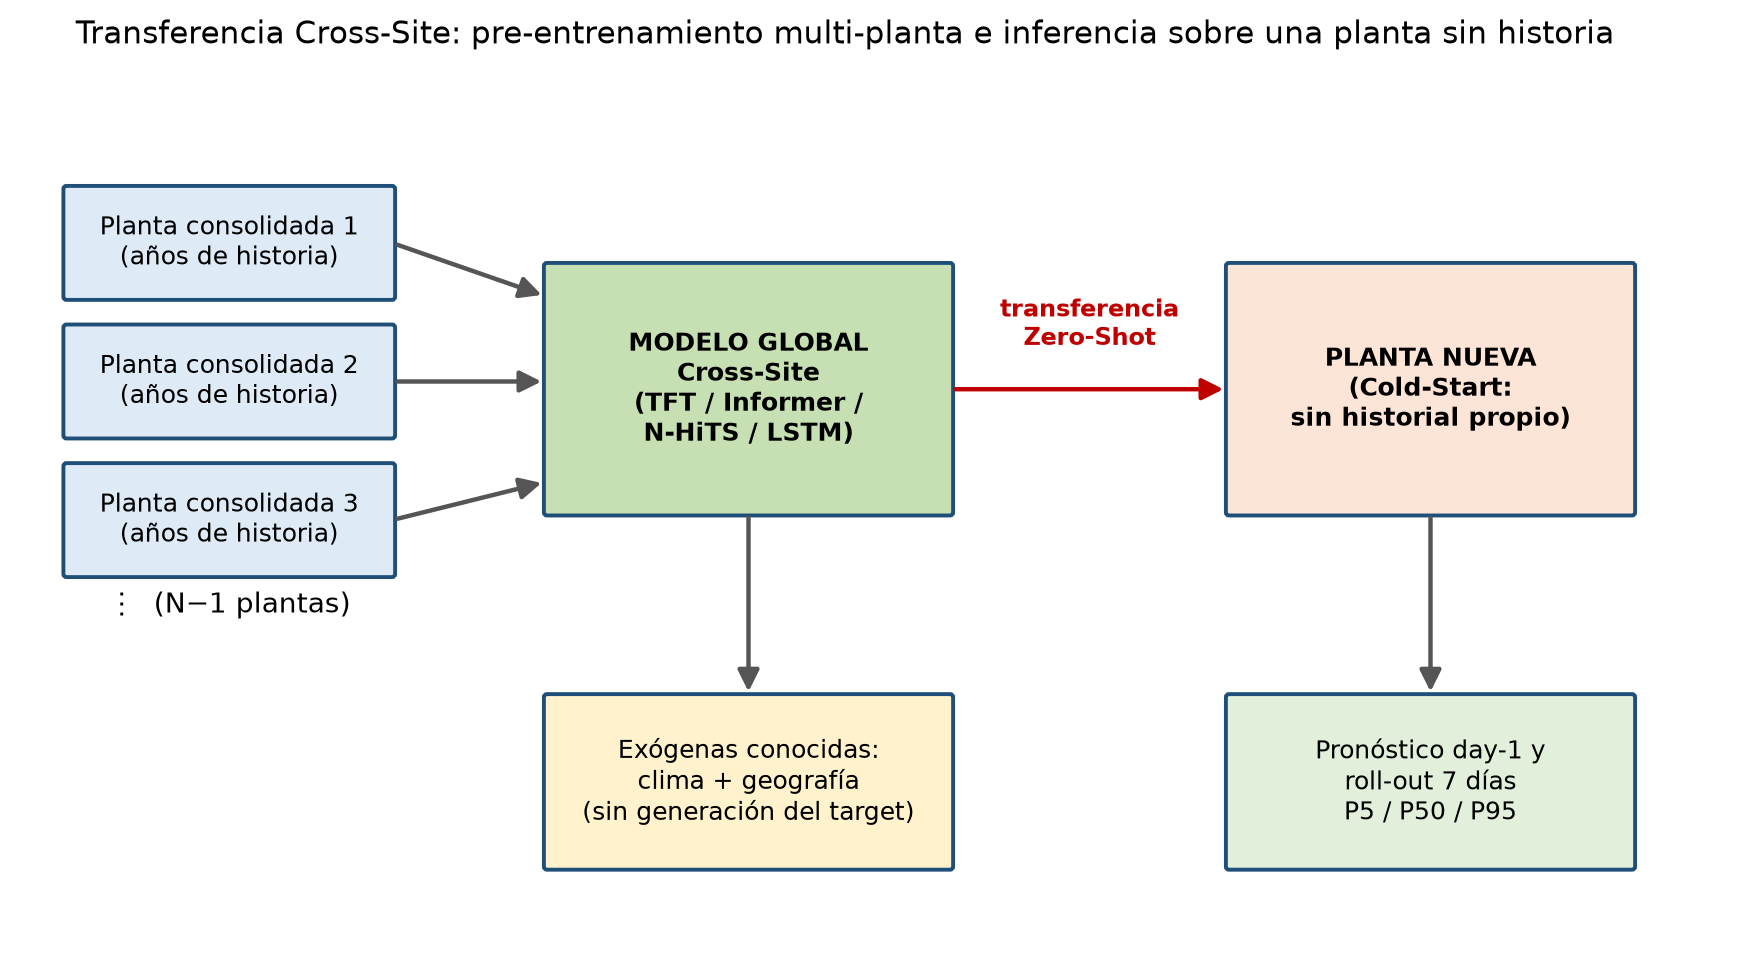
\includegraphics[width=\linewidth]{fig_solucion.png}
    \end{column}
  \end{columns}
\end{frame}

\begin{frame}{Hipótesis y objetivos}
  \begin{block}{Hipótesis}
    El modelo global multi-sitio es \emph{más preciso} que un modelo entrenado localmente con la historia propia del centro.
  \end{block}
  \begin{columns}[T]
    \begin{column}{0.5\textwidth}
      \textbf{Objetivos específicos}
      \begin{enumerate}
        \item Adaptar una arquitectura Transformer al entrenamiento multi-serie.
        \item Evaluarla frente a modelos locales bajo un protocolo \emph{Cold-Start} estricto.
        \item Integrar datos multimodales sin fuga de información.
      \end{enumerate}
    \end{column}
    \begin{column}{0.5\textwidth}
      \textbf{La brecha en la literatura}\\
      Rara vez se combinan a la vez:
      \begin{enumerate}
        \item evaluación \textbf{ciega} a la planta objetivo (sin \emph{fine-tuning}),
        \item contraste \textbf{justo} contra locales maduros,
        \item caracterización \textbf{probabilística}.
      \end{enumerate}
    \end{column}
  \end{columns}
\end{frame}

% ==================================================================
\section{Metodología}
% ==================================================================

\begin{frame}{Arquitectura del sistema}
  \centering
  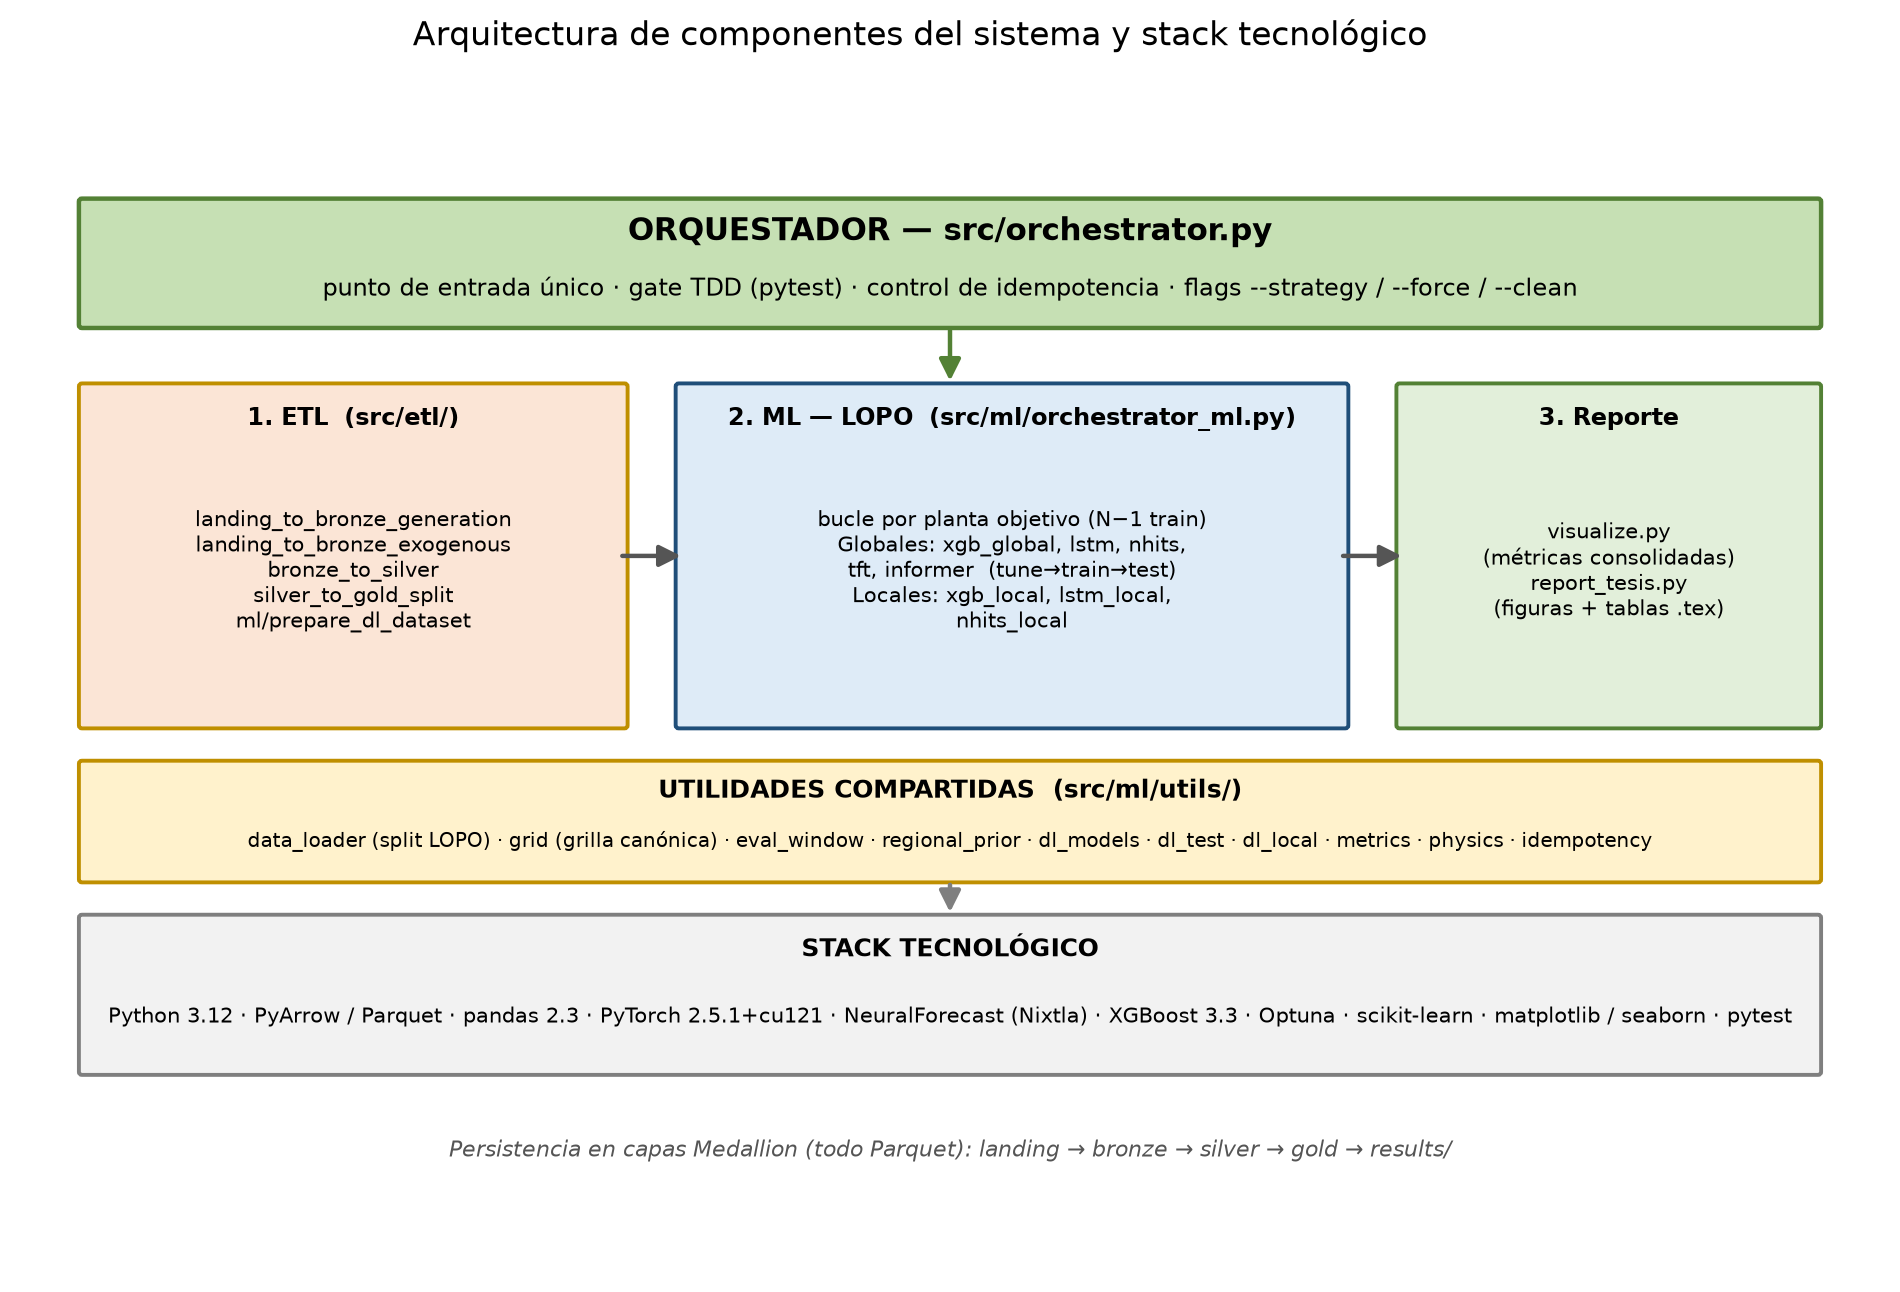
\includegraphics[height=0.78\textheight,keepaspectratio]{fig_arquitectura_componentes.png}
\end{frame}

\begin{frame}{Protocolo \emph{Leave-One-Plant-Out} (LOPO)}
  \begin{columns}[T]
    \begin{column}{0.52\textwidth}
      \begin{itemize}
        \item Para cada planta objetivo: los globales entrenan con las \textbf{$N-1$ restantes} (2014--2024 completo).
        \item La planta objetivo es \rj{invisible} durante el entrenamiento.
        \item Métricas: \textbf{mediana} sobre 94 plantas, solo observaciones reales.
      \end{itemize}
      \begin{exampleblock}{Integridad Zero-Shot (no negociable)}
        Ninguna variable puede ser función de la generación del objetivo. Verificado por pruebas automatizadas.
      \end{exampleblock}
    \end{column}
    \begin{column}{0.48\textwidth}
      \centering
      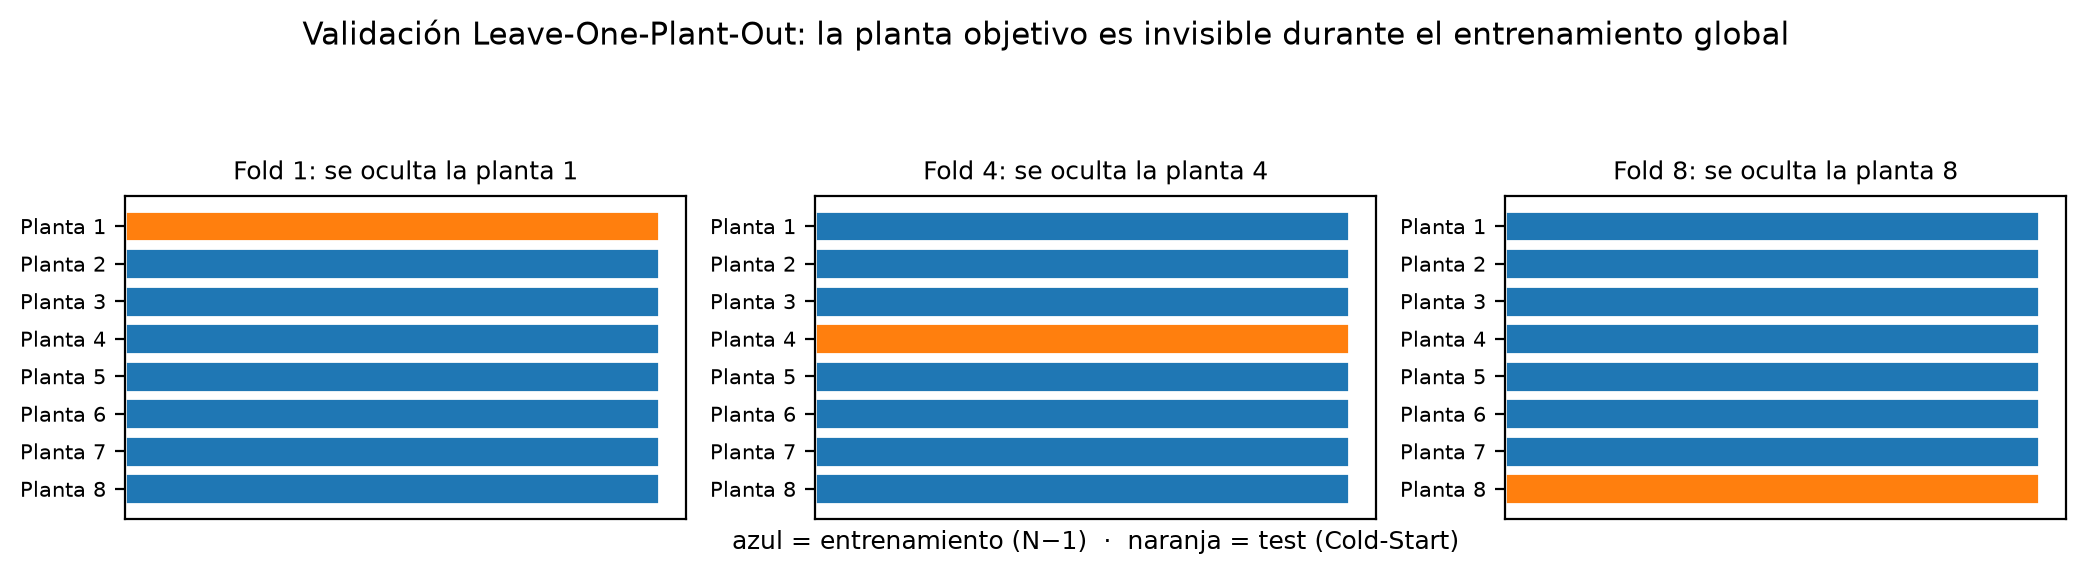
\includegraphics[width=\linewidth]{fig_lopo.png}
    \end{column}
  \end{columns}
\end{frame}

\begin{frame}{La lección de la fuga de datos}
  \begin{center}
    \Large Un \emph{prior} de eficiencia calculado \textbf{por-fila} desde el objetivo
  \end{center}
  \vspace{0.3em}
  \[
    PR = \frac{y}{\text{capacidad}} \quad\Longrightarrow\quad \mathrm{corr}(PR,\,y)=1.0
  \]
  \vspace{0.2em}
  \begin{columns}[T]
    \begin{column}{0.5\textwidth}
      \begin{alertblock}{rRMSE falso}
        $\approx 0.8\,\%$ \; (demasiado bueno para ser verdad)
      \end{alertblock}
    \end{column}
    \begin{column}{0.5\textwidth}
      \begin{exampleblock}{rRMSE honesto (tras corregir)}
        $\approx 56\,\%$
      \end{exampleblock}
    \end{column}
  \end{columns}
  \vspace{0.6em}
  \centering
  El \emph{prior} regional se agrega \textbf{solo sobre las plantas de entrenamiento} (por macrozona y estación).
\end{frame}

\begin{frame}{Semilla \emph{Cold-Start} sintética}
  Los modelos profundos necesitan una ventana de contexto que la planta nueva no tiene. Se siembra sintéticamente:
  \[
    \hat{y}_{\text{seed}}(t) = \text{capacidad}\cdot PR_{\text{regional}}\cdot s(t)
  \]
  \begin{itemize}
    \item $s(t)$: perfil solar determinista; $PR_{\text{regional}}$: solo plantas de entrenamiento.
    \item Solo el clima exógeno (conocido/pronosticable) y la geografía estática usan valores reales del objetivo.
    \item La generación de contexto es \rj{100\% sintética} $\rightarrow$ cero fuga.
  \end{itemize}
  \vspace{-0.4em}
  \centering
  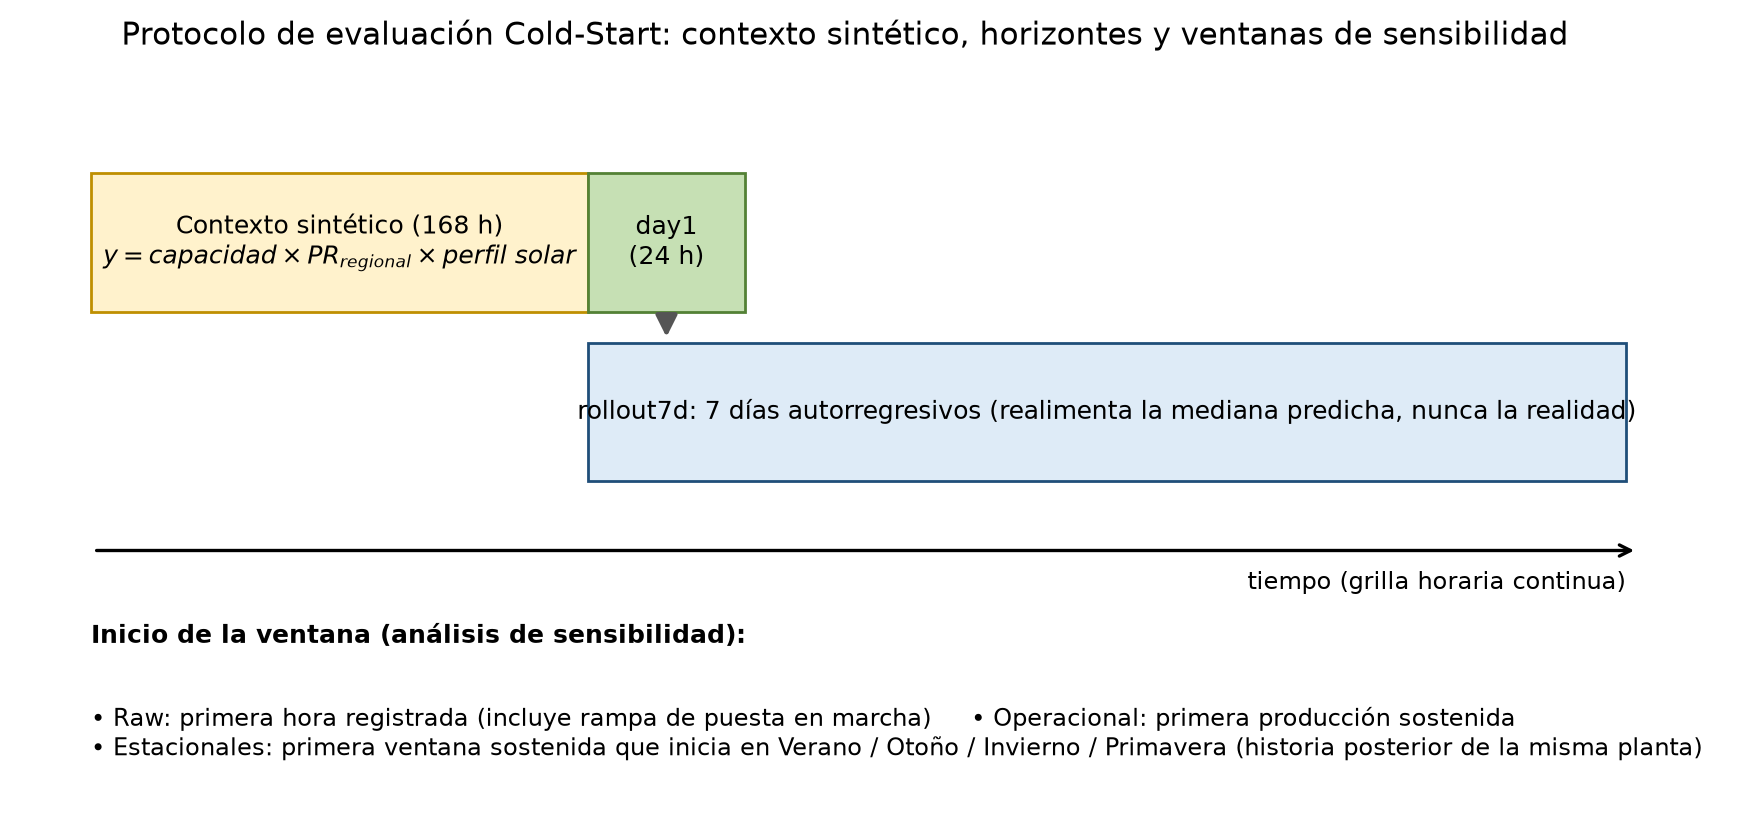
\includegraphics[width=0.54\textwidth]{fig_eval_protocolo.png}
\end{frame}

\begin{frame}{Ocho configuraciones y ventanas de evaluación}
  \begin{columns}[T]
    \begin{column}{0.48\textwidth}
      \textbf{5 globales \gl{(Cross-Site)}}
      \begin{itemize}
        \item TFT, Informer, N-HiTS, LSTM
        \item XGBoost global
      \end{itemize}
      \vspace{0.4em}
      \textbf{3 locales \lo{(estrictas)}}
      \begin{itemize}
        \item XGBoost, LSTM, N-HiTS
        \item entrenados solo con la historia propia
      \end{itemize}
      \vspace{0.5em}
      \textbf{Horizontes:} \emph{day1} (24\,h) y \emph{rollout7d} (7 días autorregresivos).
    \end{column}
    \begin{column}{0.52\textwidth}
      \centering
      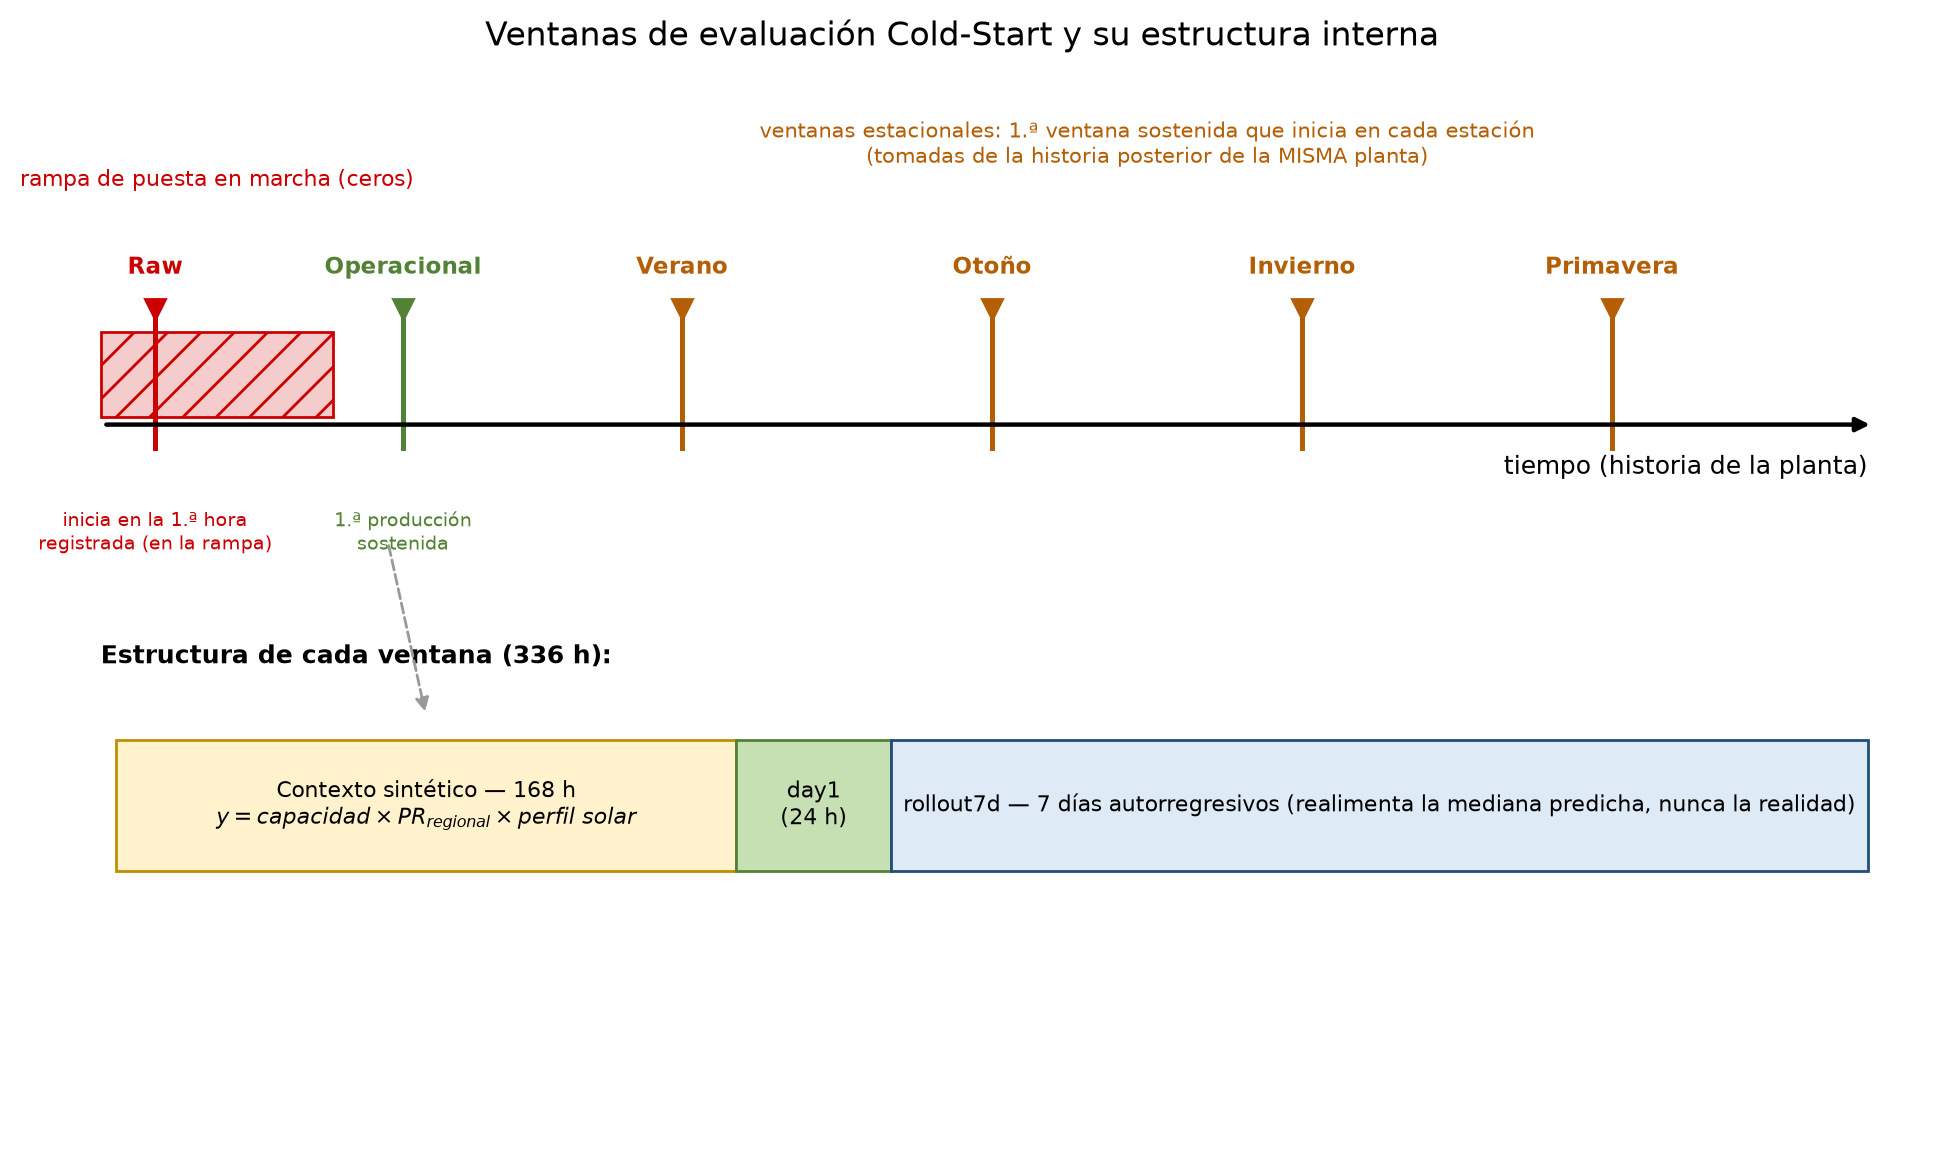
\includegraphics[width=\linewidth]{fig_ventanas_evaluacion.png}
      \vspace{0.2em}

      {\footnotesize \textbf{Raw} (incluye rampa) · \textbf{Operacional} (producción sostenida) · \textbf{Estacionales}.}
    \end{column}
  \end{columns}
\end{frame}

\begin{frame}{¿Dónde están las plantas? El corpus sobre el mapa}
  \begin{columns}[T]
    \begin{column}{0.42\textwidth}
      \centering
      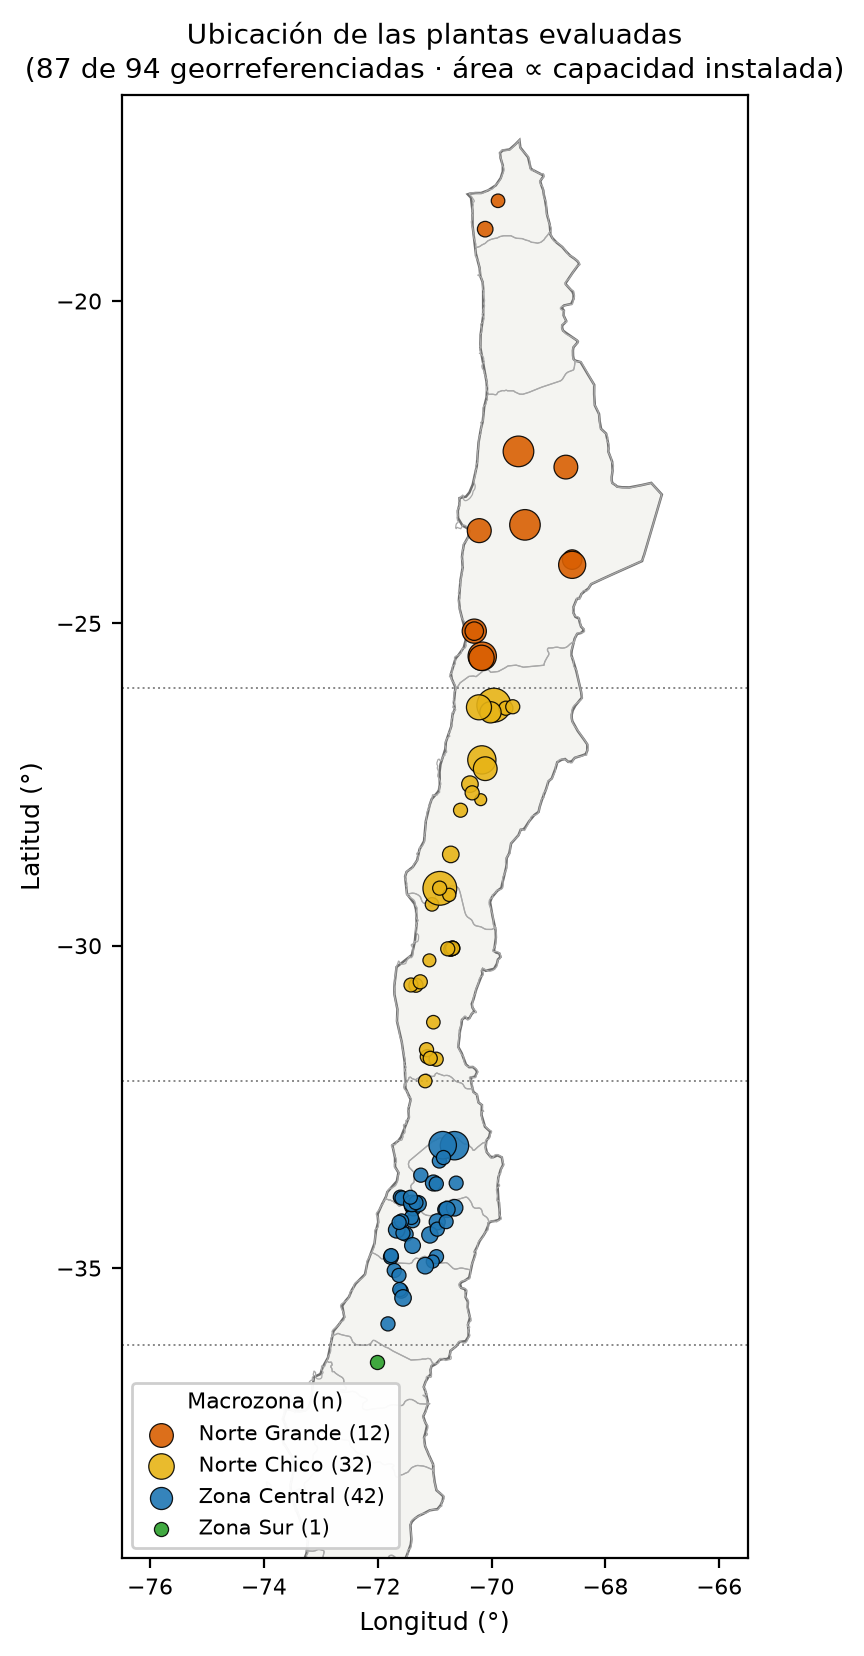
\includegraphics[height=0.78\textheight]{fig_mapa_plantas.png}
    \end{column}
    \begin{column}{0.58\textwidth}
      \vspace{1.2em}
      \begin{itemize}
        \item \textbf{94 plantas} del Sistema Eléctrico Nacional, a lo largo de todo el
              gradiente solar de Chile (Arica $\rightarrow$ zona sur).
        \item \gl{Norte Grande y Norte Chico}: pocas plantas pero \textbf{grandes}
              (utility scale, hasta 200\,MW) y de alta irradiancia.
        \item \lo{Zona Central}: muchas plantas \textbf{pequeñas} (PMGD, mediana
              $\approx$3\,MW) — el segmento que más sufre el arranque en frío.
      \end{itemize}
      \vspace{0.4em}
      \begin{exampleblock}{Por qué importa para la transferencia}
        La \textbf{macrozona} es la única señal espacial que ven los modelos, y es la
        clave sobre la que se agrega el \emph{prior} regional que siembra el contexto
        sintético.
      \end{exampleblock}
    \end{column}
  \end{columns}
\end{frame}

% ==================================================================
\section{Resultados}
% ==================================================================

\begin{frame}{Precisión puntual --- ventana \emph{cold-start}, 94 plantas (roll-out 7 días)}
  \begin{columns}[T]
    \begin{column}{0.46\textwidth}
      \small
      \begin{tabular}{llrr}
        \toprule
        Config. & Tipo & NRMSE & rRMSE \\
        \midrule
        XGBoost & \lo{Local}  & \textbf{13,2\,\%} & 60\,\% \\
        XGBoost & \gl{Global} & 17,1\,\% & 75\,\% \\
        N-HiTS  & \lo{Local}  & 17,6\,\% & 85\,\% \\
        Informer& \gl{Global} & 22,8\,\% & 107\,\% \\
        TFT     & \gl{Global} & 23,6\,\% & 113\,\% \\
        LSTM    & \lo{Local}  & 23,9\,\% & 129\,\% \\
        LSTM    & \gl{Global} & 24,8\,\% & 109\,\% \\
        N-HiTS  & \gl{Global} & 30,7\,\% & 148\,\% \\
        \bottomrule
      \end{tabular}

      \vspace{0.3em}
      {\scriptsize NRMSE = RMSE / capacidad instalada. \textbf{94 plantas}.}
    \end{column}
    \begin{column}{0.54\textwidth}
      \centering
      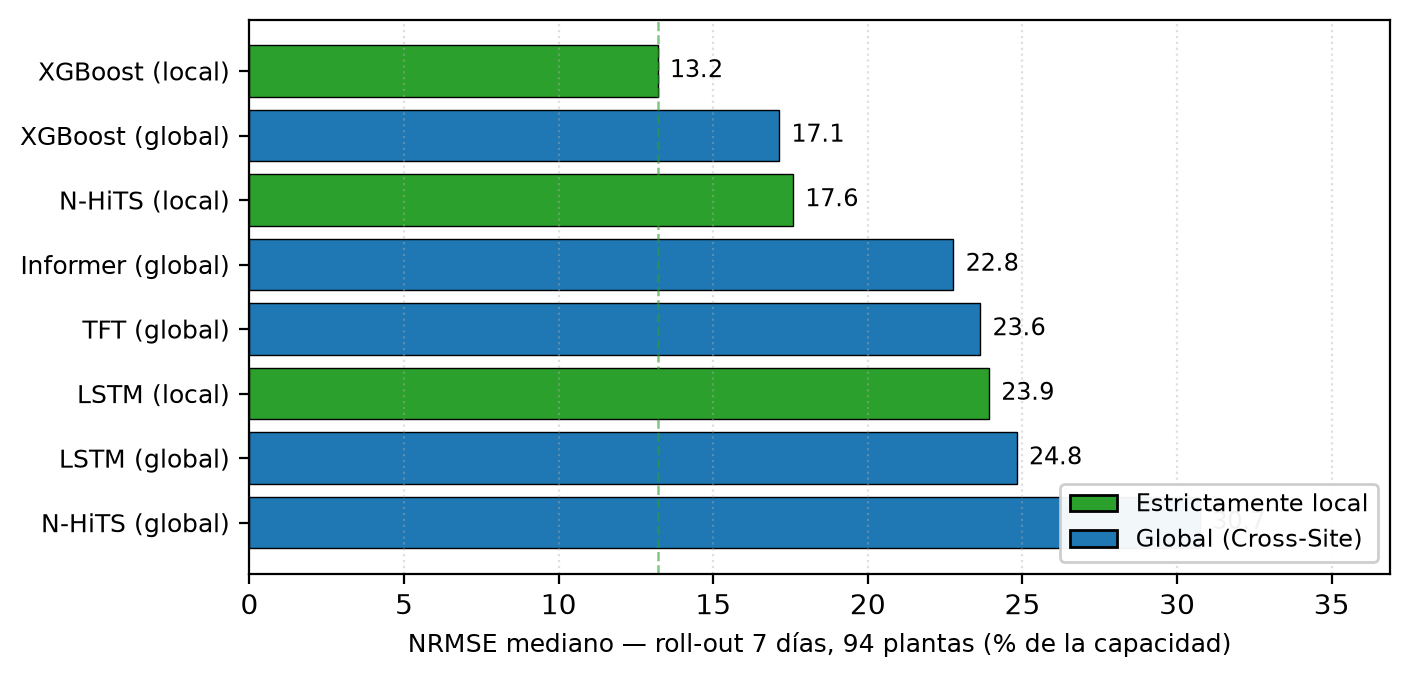
\includegraphics[width=\linewidth]{fig_resultados_nrmse_es.png}
    \end{column}
  \end{columns}
  \vspace{0.2em}
  {\footnotesize El \lo{XGBoost local} es el más preciso (13\,\% de la potencia nominal). Normalizar por \textbf{capacidad} hace los números interpretables —y cambia el orden del par LSTM respecto de rRMSE.}
\end{frame}

\begin{frame}{Sensibilidad estacional: el invierno es el gran desafío}
  \begin{columns}[T]
    \begin{column}{0.5\textwidth}
      \centering
      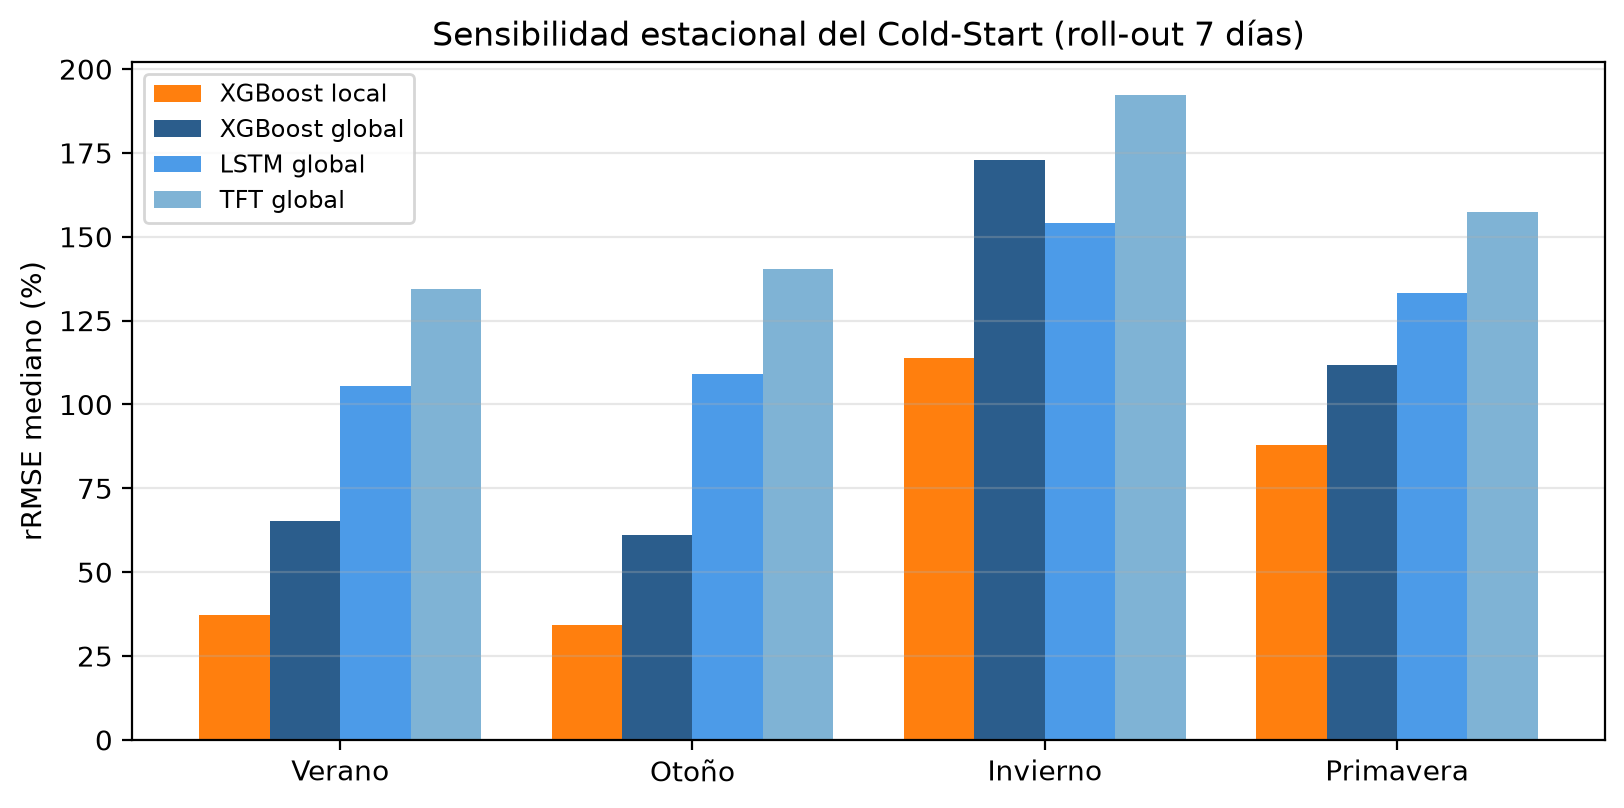
\includegraphics[width=\linewidth]{fig_estacional.png}
    \end{column}
    \begin{column}{0.5\textwidth}
      \textbf{rRMSE roll-out por estación}
      \vspace{0.3em}

      \begin{itemize}
        \item XGBoost global: \; 52\,\% (verano) $\rightarrow$ \rj{134\,\%} (invierno)
        \item XGBoost local: \; 40\,\% $\rightarrow$ \rj{115\,\%}
      \end{itemize}
      \vspace{0.5em}
      Mayor variabilidad nubosa y menor irradiación invernal debilitan la señal determinista del perfil solar.
      \vspace{0.5em}

      \textbf{Implicación operativa:} la incertidumbre de un parque nuevo depende fuertemente de la \textbf{estación de su puesta en marcha}.
    \end{column}
  \end{columns}
\end{frame}

\begin{frame}{Calidad probabilística: la calibración no se transfiere}
  \small
  \begin{center}
  \begin{tabular}{llcc}
    \toprule
    Config. & Tipo & Cobertura diurna & Pinball P95 (MWh) \\
    \midrule
    XGBoost  & \lo{Local}  & \textbf{0,86} & \textbf{0,035} \\
    XGBoost  & \gl{Global} & 0,97 (sobre-cubre) & 0,092 \\
    LSTM     & \gl{Global} & 0,53 & 0,159 \\
    Informer & \gl{Global} & 0,64 & 0,115 \\
    TFT      & \gl{Global} & 0,38 & 0,158 \\
    N-HiTS   & \gl{Global} & 0,37 & 0,372 \\
    \bottomrule
  \end{tabular}
  \end{center}
  \normalsize
  \begin{itemize}
    \item Nominal = 0,90. \textbf{Ningún paradigma calibra idealmente}, con desvíos opuestos.
    \item Redes globales \rj{subcalibradas} (bandas demasiado estrechas); XGBoost global \rj{sobre-cubre}.
    \item \lo{XGBoost local} es el más cercano al nominal y con menor pinball.
  \end{itemize}
\end{frame}

\begin{frame}{Contraste de la hipótesis --- con test estadístico}
  % OJO: dentro de un título de bloque NO usar \rj/\lo/\gl — el fondo ya es de color
  % y el texto quedaría invisible (rojo sobre rojo). Se usa negrita sobre el blanco heredado.
  \begin{alertblock}{La hipótesis se \textbf{RECHAZA}, y ahora con significancia}
    \lo{XGBoost local} gana a \gl{XGBoost global} en \textbf{77 de 94 plantas}
    ($p<10^{-7}$, Wilcoxon pareado con corrección de Holm).
  \end{alertblock}
  \begin{block}{A igualdad de arquitectura: ningún global gana significativamente}
    \begin{itemize}
      \item \lo{N-HiTS local} supera a \gl{N-HiTS global} en \textbf{88/94} ($p<10^{-10}$).
      \item El par \textbf{LSTM} es un \rj{empate estadístico}: 49/45 plantas, $p=1{,}00$.
            El matiz que sugerían las medianas \textbf{no sobrevive} al test pareado.
    \end{itemize}
  \end{block}
  \begin{exampleblock}{El valor real: disponibilidad inmediata}
    En el arranque en frío puro (historia local nula) el modelo global \textbf{no tiene competidor local posible}.
  \end{exampleblock}
\end{frame}

\begin{frame}{Ejemplo de roll-out Cold-Start a 7 días}
  \centering
  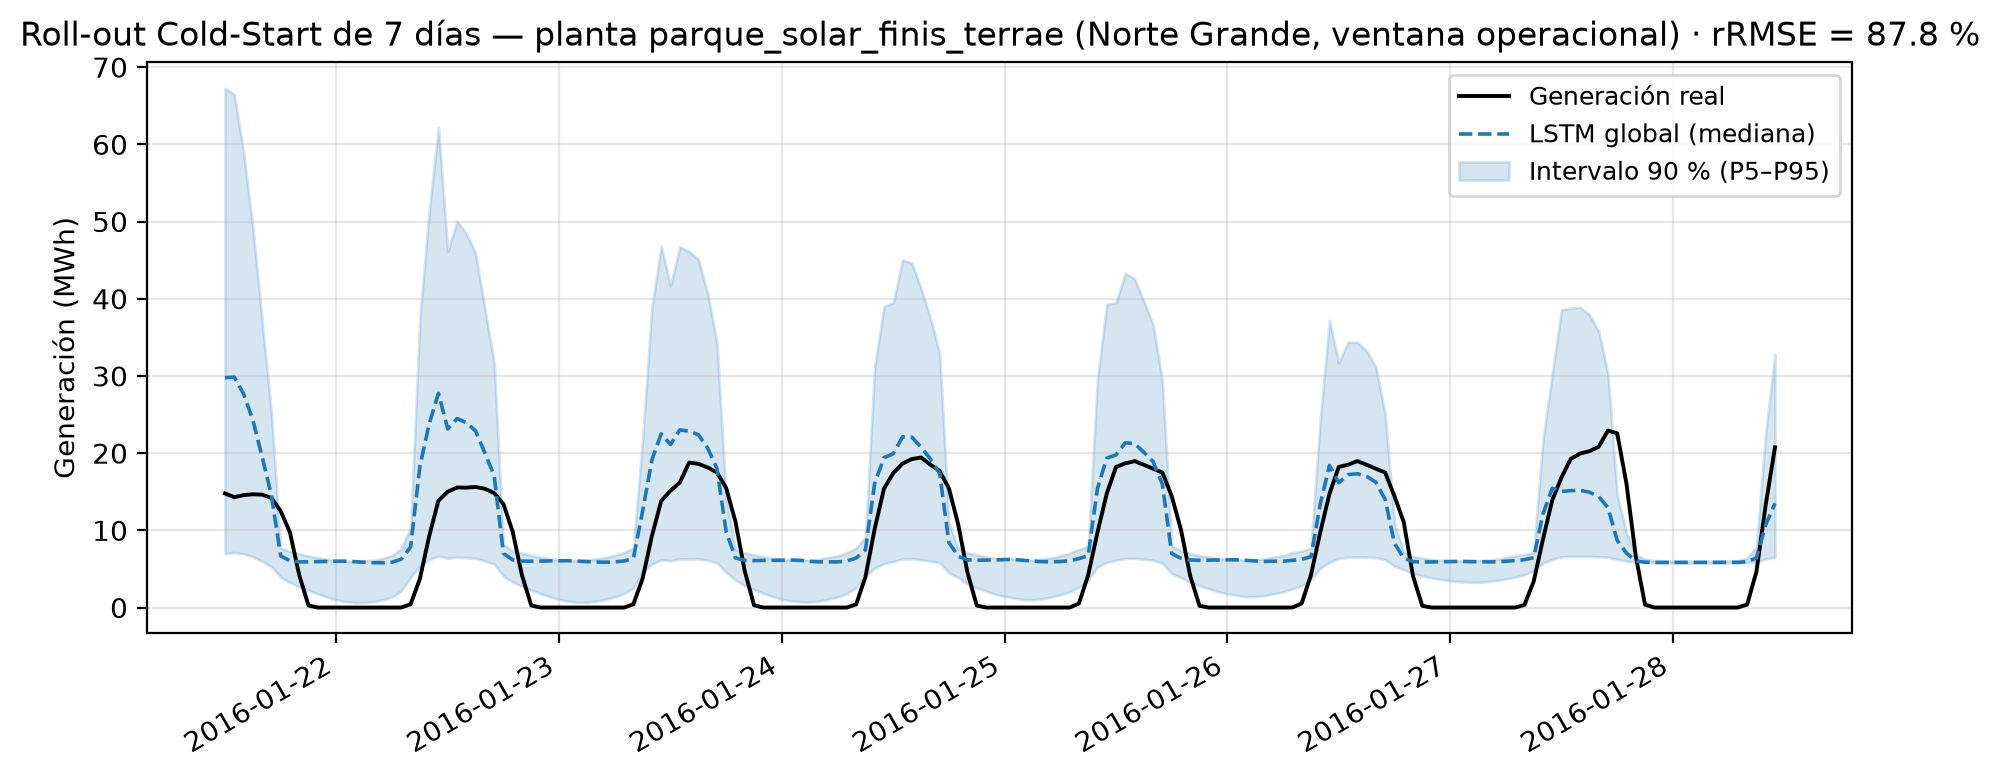
\includegraphics[width=0.9\textwidth]{fig_ejemplo_rollout.png}

  {\footnotesize El modelo global, \textbf{sin haber visto jamás la planta}, reproduce el ciclo diario y la magnitud de los picos usando solo el clima entrante y la geografía estática.}
\end{frame}

% ==================================================================
\section{Conclusiones}
% ==================================================================

\begin{frame}{Conclusiones}
  \begin{enumerate}
    \item \textbf{Resultado negativo riguroso:} bajo un protocolo estrictamente ciego, un XGBoost local maduro sigue siendo el estándar a batir. La hipótesis se rechaza.
    \item \textbf{El paradigma global conserva un régimen propio:} el arranque en frío puro, donde entrega pronósticos coherentes y accionables desde la hora cero.
    \item Cuatro hallazgos metodológicos transferibles:
    \begin{itemize}
      \item las rampas de puesta en marcha distorsionan las métricas (análisis Raw/Operacional);
      \item el invierno es sistemáticamente la estación más difícil;
      \item la calibración probabilística no se transfiere a las redes profundas;
      \item la integridad del \emph{target} (nunca imputar $y$) es esencial para la honestidad de las métricas.
    \end{itemize}
  \end{enumerate}
\end{frame}

\begin{frame}{Trabajo futuro}
  \begin{itemize}
    \item \textbf{Fine-tuning en dos etapas:} pre-entrenar global $\rightarrow$ ajustar con los primeros días reales; cierra la brecha con el local a medida que crece la historia.
    \item \textbf{Máscaras de intermitencia} en la atención: excluir la noche determinista y concentrar capacidad en la señal productiva.
    \item \textbf{Recalibración conformal} de los intervalos bajo transferencia.
    \item \textbf{Más datos y cómputo:} ampliar el corpus y el presupuesto de pasos (posible sub-entrenamiento de TFT/Informer en 6\,GB).
    \item \textbf{Máscara astronómica} para el forzamiento nocturno independiente de sensores.
  \end{itemize}
\end{frame}

\begin{frame}[plain]
  \centering
  \vfill
  {\usebeamercolor[fg]{structure}\Huge \textbf{Gracias}}\\[0.5em]
  {\Large ¿Preguntas?}\\[1.0em]
  
\includegraphics[width=0.13\linewidth]{figuras/logoUCM.png}\\[0.5em]
  \ifnum\confmode=1
    {\normalsize César David Aular Muñoz \quad·\quad Sergio Hernández}\\
    {\footnotesize cesaraular02@gmail.com \quad·\quad Universidad Católica del Maule}
  \else
    {\normalsize César David Aular Muñoz}\\
    {\footnotesize cesaraular02@gmail.com}
  \fi
  \vfill
\end{frame}

% ==================================================================
% BACKUP SLIDES — anticipando los ataques de la comisión
% ==================================================================
\appendix

\begin{frame}{Backup --- Tests estadísticos (Friedman + Wilcoxon-Holm)}
  \textbf{Diseño pareado y balanceado:} 94 plantas $\times$ 8 configuraciones sobre la
  misma grilla horaria canónica $\rightarrow$ aplica la comparación por rangos de
  Demšar (2006).
  \vspace{0.3em}
  \begin{itemize}
    \item \textbf{Friedman (omnibus):} $\chi^2 = 260{,}7$, $p < 10^{-50}$ — las
          configuraciones no son equivalentes.
    \item \textbf{Ranking medio} (1 = mejor): XGB local 1,80 · N-HiTS local 3,32 ·
          XGB global 3,34 · TFT 5,10 · Informer 5,15 · LSTM local 5,30 ·
          LSTM global 5,41 · N-HiTS global 6,59.
    \item \textbf{Mejor por planta:} XGB local en 60/94, XGB global en 15,
          N-HiTS local en 10.
  \end{itemize}
  \vspace{0.2em}
  \begin{alertblock}{Por qué la mediana marginal engañaba}
    rRMSE mediano sugería \gl{LSTM global} (118\,\%) mejor que \lo{LSTM local}
    (147\,\%). Pero la \textbf{mediana de las diferencias por planta} es $\approx 0$ y
    levemente a favor del local: la brecha la producían unas pocas plantas donde el
    local falla mucho, no una ventaja sistemática del global.
  \end{alertblock}
\end{frame}

\begin{frame}{Backup --- Causalidad temporal de los baselines locales}
  \begin{block}{Qué se hizo exactamente}
    Los baselines locales se entrenan con la historia \textbf{completa} de la planta
    \textbf{menos todas las ventanas de evaluación} (Raw, Operacional y las 4
    estacionales), con los \emph{lags} hacia esas ventanas enmascarados.
  \end{block}
  \begin{itemize}
    \item No hay fuga del \emph{target}: ningún rezago apunta dentro de una ventana.
    \item Pero el entrenamiento \textbf{sí incluye horas posteriores} a la ventana
          predicha $\rightarrow$ \rj{no es estrictamente causal}.
    \item Es una elección de diseño: representa el modelo maduro que el operador
          tendría \emph{tras acumular historia} — el rival más fuerte posible.
  \end{itemize}
  \begin{exampleblock}{Por qué esto refuerza la conclusión}
    El sesgo favorece al lado \lo{local}, que \textbf{gana}; y el espejo (LOPO oculta
    la planta pero \textbf{no el calendario}) favorece al lado \gl{global}, que
    \textbf{pierde igual}. Ambos sesgos empujan contra la conclusión reportada.
  \end{exampleblock}
\end{frame}

\begin{frame}{Backup --- Definición del RMSE}
  \begin{block}{Fórmula}
    \[
      \mathrm{RMSE} = \sqrt{\frac{1}{n}\sum_{i=1}^{n}\left(y_i - \hat{y}_i\right)^2}
    \]
  \end{block}
  \begin{itemize}
    \item Eleva al \textbf{cuadrado} cada error antes de promediar $\rightarrow$ penaliza las desviaciones grandes de forma \rj{cuadrática}, no lineal ni logarítmica.
    \item Ideal para el pronóstico FV: castiga con fuerza los errores en los \textbf{picos de inyección} de mediodía.
    \item Comparte unidades con la variable (MWh), a diferencia del MSE.
    \item \textbf{rRMSE} = RMSE normalizado por la generación media horaria de la ventana (ver backup siguiente).
  \end{itemize}
\end{frame}

\begin{frame}{Backup --- ¿Por qué el rRMSE supera el 100\,\%?}
  \[
    \mathrm{rRMSE} = \frac{\mathrm{RMSE}}{\overline{y}_{\text{ventana}}}\times 100
  \]
  \begin{itemize}
    \item El denominador $\overline{y}$ incluye las \textbf{horas nocturnas de generación nula}.
    \item Esto \textbf{deprime la media} y por tanto \textbf{infla} sistemáticamente el indicador.
    \item Valores $>100\,\%$ son \textbf{esperables} en pronóstico horario FV bajo esta normalización.
    \item Su valor no es la magnitud absoluta, sino la \rj{comparación relativa} entre arquitecturas sobre \textbf{ventanas idénticas}.
  \end{itemize}
  \vspace{0.3em}
  \centering\footnotesize
  Todas las configuraciones se comparan sobre la misma grilla horaria canónica $\rightarrow$ comparación estrictamente pareada.
\end{frame}

\begin{frame}{Backup --- Calibración de XGBoost (global vs.\ local)}
  \begin{columns}[T]
    \begin{column}{0.5\textwidth}
      \textbf{XGBoost global: 0,97 (sobre-cubre)}
      \begin{itemize}
        \item Regresión cuantílica sobre un contexto \textbf{heterogéneo} ($N-1$ plantas).
        \item Bandas \textbf{demasiado anchas}: casi nunca fallan, pero pierden utilidad operativa.
        \item Un defecto \textbf{simétrico} al de las redes, no una virtud.
      \end{itemize}
    \end{column}
    \begin{column}{0.5\textwidth}
      \textbf{XGBoost local: 0,86 (casi nominal)}
      \begin{itemize}
        \item Ajustado a la variabilidad \textbf{real} de la propia planta.
        \item Pinball P95 = \textbf{0,035} MWh vs.\ 0,092 del global.
        \item Intervalos más estrechos y \textbf{mejor centrados}.
      \end{itemize}
    \end{column}
  \end{columns}
  \vspace{0.5em}
  \begin{alertblock}{¿Por qué las redes profundas subcalibran?}
    Su escalador local se ajusta sobre el \textbf{contexto sintético}, cuya varianza (perfil solar idealizado) es menor que la real $\rightarrow$ bandas estrechas. Los baselines locales profundos, con contexto real, mejoran (LSTM local 0,79).
  \end{alertblock}
\end{frame}

\begin{frame}{Backup --- Detalles de cómputo}
  \begin{itemize}
    \item \textbf{Precisión fp32} completa: la mezcla fp16 introducía inestabilidad numérica en el entrenamiento.
    \item \textbf{GPU RTX 2060 (6\,GB):} la VRAM la gobierna \texttt{batch\_size}$\times$\texttt{windows\_batch\_size}, no el tamaño del corpus $\rightarrow$ no se trunca la historia.
    \item \textbf{Presupuesto por época corregido:} cada paso consume \texttt{batch}$\times$\texttt{windows\_batch} ventanas; la fórmula ingenua \texttt{filas/batch} sobreestimaba $\sim$250$\times$.
    \item \textbf{\emph{Early stopping}} sobre \texttt{val\_size}=168; tuning cacheado una vez por modelo y reusado entre folds (fuga a nivel de hiperparámetro: despreciable y documentada).
    \item Toda predicción se fuerza a $\hat{y}\geq 0$ y a cero de noche (consistencia física).
  \end{itemize}
\end{frame}

\begin{frame}{Backup --- Tabla completa (day1 y roll-out)}
  \scriptsize
  \begin{center}
  \begin{tabular}{llcccccc}
    \toprule
     & & \multicolumn{2}{c}{NRMSE (\% cap.)} & \multicolumn{2}{c}{rRMSE (\%)} & & \\
    \cmidrule(lr){3-4}\cmidrule(lr){5-6}
    Config. & Tipo & day1 & roll7d & day1 & roll7d & Cob. & Pinball \\
    \midrule
    XGBoost  & \lo{Local}  & \textbf{9,5} & \textbf{13,2} & 45,6 & 59,9 & 0,86 & 0,035 \\
    XGBoost  & \gl{Global} & 15,6 & 17,1 & 64,0 & 75,1 & 0,97 & 0,092 \\
    N-HiTS   & \lo{Local}  & 14,2 & 17,6 & 62,3 & 85,2 & 0,72 & 0,096 \\
    Informer & \gl{Global} & 21,0 & 22,8 & 96,6 & 106,5 & 0,64 & 0,115 \\
    TFT      & \gl{Global} & 22,0 & 23,6 & 105,1 & 112,7 & 0,38 & 0,158 \\
    LSTM     & \lo{Local}  & 16,3 & 23,9 & 102,6 & 128,8 & 0,72 & 0,235 \\
    LSTM     & \gl{Global} & 22,6 & 24,8 & 99,7 & 108,6 & 0,53 & 0,159 \\
    N-HiTS   & \gl{Global} & 28,6 & 30,7 & 129,8 & 148,2 & 0,37 & 0,372 \\
    \bottomrule
  \end{tabular}
  \end{center}
  \normalsize
  \centering Ventana \emph{cold-start}, mediana sobre las \textbf{94 plantas}
  (Operacional donde hay rampa $>$24\,h; Raw en el resto).
\end{frame}

\end{document}
